%%%%%%%%%%%%%%
%% Run LaTeX on this file several times to get Table of Contents,
%% cross-references, and citations.

%% w-bktmpl.tex. Current Version: Feb 16, 2012
%%%%%%%%%%%%%%%%%%%%%%%%%%%%%%%%%%%%%%%%%%%%%%%%%%%%%%%%%%%%%%%%
%
%  Template file for
%  Wiley Book Style, Design No.: SD 001B, 7x10
%  Wiley Book Style, Design No.: SD 004B, 6x9
%
%  Prepared by Amy Hendrickson, TeXnology Inc.
%  http://www.texnology.com
%%%%%%%%%%%%%%%%%%%%%%%%%%%%%%%%%%%%%%%%%%%%%%%%%%%%%%%%%%%%%%%%

%%%%%%%%%%%%%%%%%%%%%%%%%%%%%%%%%%%%%%%%%%%%%%%%%%%%%%%%%%%%%%%%
%% Class File

%% For default 7 x 10 trim size:
%\documentclass{WileySev}

%% Or, for 6 x 9 trim size
\documentclass{WileySix}

%%%%%%%%%%%%%%%%%%%%%%%%%%%%%%%%%%%%%%%%%%%%%%%%%%%%%%%%%%%%%%%%
%% Post Script Font File

% For PostScript text
% If you have font problems, you may edit the w-bookps.sty file
% to customize the font names to match those on your system.

\usepackage{w-bookps}

%%%%%%%
%% For times math: However, this package disables bold math (!)
%% \mathbf{x} will still work, but you will not have bold math
%% in section heads or chapter titles. If you don't use math
%% in those environments, mathptmx might be a good choice.

% \usepackage{mathptmx}


%%%%%%%%%%%%%%%%%%%%%%%%%%%%%%%%%%%%%%%%%%%%%%%%%%%%%%%%%%%%%%%%
%% Graphicx.sty for Including PostScript .eps files

\usepackage{graphicx}


%%%%%%%%%%%%%%%%%%%%%%%%%%%%%%%%%%%%%%%%%%%%%%%%%%%%%%%%%%%%%%%%
%% Other packages you might want to use:

% for chapter bibliography made with BibTeX
% \usepackage{chapterbib}

% for multiple indices
% \usepackage{multind}

% for answers to problems
% \usepackage{answers}




%%%%%%%%%%%%%%%%%%%%%%%%%%%%%%%%%%%%%%%%%%%%%%%%%%%%%%%%%%%%%%%%
%% Change options here if you want:
%%
%% How many levels of section head would you like numbered?
%% 0= no section numbers, 1= section, 2= subsection, 3= subsubsection
%%==>>
\setcounter{secnumdepth}{3}

%% How many levels of section head would you like to appear in the
%% Table of Contents?
%% 0= chapter titles, 1= section titles, 2= subsection titles, 
%% 3= subsubsection titles.
%%==>>
\setcounter{tocdepth}{2}

%% Cropmarks? good for final page makeup
%% \docropmarks %% turn cropmarks on

%%%%%%%%%%%%%%%%%%%%%%%%%%%%%%%%%%%%%%%%%%%%%%%%%%%%%%%%%%%%%%%%
%% DRAFT
%
% Uncomment to get double spacing between lines, current date and time
% printed at bottom of page.
% \draft
% (If you want to keep tables from becoming double spaced also uncomment
% this):
% \renewcommand{\arraystretch}{0.6}
%%%%%%%%%%%%%%%%%%%%%%%%%%%%%%

\begin{document}

%%%%%%%%%%%%%%%%%%%%%%%%%%%%%%%%%%%%%%%%%%%%%%%%%%%%%%%%%%%%%%%%
%% Title Pages
%%
%% Wiley will provide title and copyright page, but you can make
%% your own titlepages if you'd like anyway

%% Setting up title pages, type in the appropriate names here:
\booktitle{Sistem Informasi Geografis}
\subtitle{Mengenal dan Membangun SIG}

\author{Rolly Maulana Awangga}
%\affil{Program Studi Sarjana Terapan Teknik Informatika Politeknik Pos Indonesia}
%or
%\authors{}

%% \\ will start a new line.
%% You may add \affil{} for affiliation, ie,
%\authors{Robert M. Groves\\
%\affil{Universitat de les Illes Balears}
%Floyd J. Fowler, Jr.\\
%\affil{University of New Mexico}
%}

%% Print Half Title and Title Page:
\halftitlepage
\titlepage


%%%%%%%%%%%%%%%%%%%%%%%%%%%%%%%%%%%%%%%%%%%%%%%%%%%%%%%%%%%%%%%%
%% Off Print Info

%% Add your info here:
\offprintinfo{Sistem Informasi Geografis, pre-release}{Rolly Maulana Awangga}

%% Can use \\ if title, and edition are too wide, ie,
%% \offprintinfo{Survey Methodology,\\ Second Edition}{Robert M. Groves}


%%%%%%%%%%%%%%%%%%%%%%%%%%%%%%%%%%%%%%%%%%%%%%%%%%%%%%%%%%%%%%%%
%% Copyright Page

\begin{copyrightpage}{2017}
Sistem Informasi Geografis / Rolly Maulana Awangga
\end{copyrightpage}

% Note, you must use \ to start indented lines, ie,
% 
% \begin{copyrightpage}{2004}
% Survey Methodology / Robert M. Groves . . . [et al.].
% \       p. cm.---(Wiley series in survey methodology)
% \    ``Wiley-Interscience."
% \    Includes bibliographical references and index.
% \    ISBN 0-471-48348-6 (pbk.)
% \    1. Surveys---Methodology.  2. Social 
% \  sciences---Research---Statistical methods.  I. Groves, Robert M.  II. %
% Series.\\

% HA31.2.S873 2004
% 001.4'33---dc22                                             2004044064
% \end{copyrightpage}

%%%%%%%%%%%%%%%%%%%%%%%%%%%%%%%%%%%%%%%%%%%%%%%%%%%%%%%%%%%%%%%%
%% Frontmatter >>>>>>>>>>>>>>>>

%%%%%%%%%%%%%%%%%%%%%%%%%%%%%%%%%%%%%%%%%%%%%%%%%%%%%%%%%%%%%%%%
%% Only Dedication (optional) 
%% or Contributor Page for edited books
%% before \tableofcontents

\dedication{For my family}

% ie,
%\dedication{To my parents}

%%%%%%%%%%%%%%%%%%%%%%%%%%%%%%%%%%%%%%%%%%%%%%%%%%%%%%%%%%%%%%%%
%  Contributors Page for Edited Book
%%%%%%%%%%%%%%%%%%%%%%%%%%%%%%%%%%%%%%%%%%%%%%%%%%%%%%%%%%%%%%%%

% If your book has chapters written by different authors,
% you'll need a Contributors page.

% Use \begin{contributors}...\end{contributors} and
% then enter each author with the \name{} command, followed
% by the affiliation information.

% \begin{contributors}
% \name{Masayki Abe,} Fujitsu Laboratories Ltd., Fujitsu Limited, Atsugi,
% Japan

% \name{L. A. Akers,} Center for Solid State Electronics Research, Arizona
% State University, Tempe, Arizona

% \name{G. H. Bernstein,} Department of Electrical and
% Computer Engineering, University of Notre Dame, Notre Dame, South Bend, 
% Indiana; formerly of
% Center for Solid State Electronics Research, Arizona
% State University, Tempe, Arizona 
% \end{contributors}

%%%%%%%%%%%%%%%%%%%%%%%%%%%%%%%%%%%%%%%%%%%%%%%%%%%%%%%%%%%%%%%%
\contentsinbrief %optional
\tableofcontents
% \listoffigures %optional
% \listoftables  %optional

%%%%%%%%%%%%%%%%%%%%%%%%%%%%%%%%%%%%%%%%%%%%%%%%%%%%%%%%%%%%%%%%
% Optional Foreword:

%\begin{foreword}
%text
%\end{foreword}

%%%%%%%%%%%%%%%%%%%%%%%%%%%%%%%%%%%%%%%%%%%%%%%%%%%%%%%%%%%%%%%%
% Optional Preface:

%\begin{preface}
% text
%\prefaceauthor{}
%\where{place\\
% date}
%\end{preface}

% ie,
% \begin{preface}
% This is an example preface.
% \prefaceauthor{R. K. Watts}
% \where{Durham, North Carolina\\
% September, 2004}

%%%%%%%%%%%%%%%%%%%%%%%%%%%%%%%%%%%%%%%%%%%%%%%%%%%%%%%%%%%%%%%%
% Optional Acknowledgments:

% \acknowledgments
% acknowledgment text
% \authorinitials{} % ie, I. R. S.


%%%%%%%%%%%%%%%%%%%%%%%%%%%%%%%%
%% Glossary Type of Environment:

% \begin{glossary}
% \term{<term>}{<description>}
% \end{glossary}

%%%%%%%%%%%%%%%%%%%%%%%%%%%%%%%%
% \begin{acronyms} 
% \acro{<term>}{<description>}
% \end{acronyms}

%%%%%%%%%%%%%%%%%%%%%%%%%%%%%%%%
%% In symbols environment <term> is expected to be in math mode; 
%% if not in math mode, use \term{\hbox{<term>}}

% \begin{symbols}
% \term{<math term>}{<description>}
% \term{\hbox{<non math term>}}Box used when not using a math symbol.
% \end{symbols}

%%%%%%%%%%%%%%%%%%%%%%%%%%%%%%%%
% \begin{introduction}
%\introauthor{<name>}{<affil>}
% Introduction text...
% \end{introduction}

%%%%%%%%%%%%%%%%%%%%%%%%%%%%%%%%%%%%%%%%%%%%%%%%%%%%%%%%%%%%%%%%
%% End for Front Matter, Beginning of text of book  >>>>>>>>>>>

%% Short version of title without \\ may be written in sq. brackets:

%% Optional Part :
\part[Pendahuluan]
{Pendahuluan\\ Pengantar Geospasial}


%\chapter[Sejarah Ptolemy]
%{Pendahuluan\\ Ptolemy}
%<<<<<<< HEAD
% kelompok 2 tUGAS 1 GIS (Ptolemy)
%Tiara Rizki Wulansari (1154026)
% Muhamad Rifan Zamaludin (1154088)
% Mohammad Agung Deomartha (1154032)
% M. Fajri Mualim (1154078)
% Faisal Syarifuddin (1154104)

\section{Peta}
	peta adalah/merupakan penggambaran secara grafis atau bentuk skala (perbandingan) pada konsep mengenai bumi. dalam hal ini peta merupakan alat untuk menyampaikan atau menginformasikan mengenai ilmu kebumian. bagaimana peta dahulu ditemukan ? pengetahuan mengenai dasar pembentukan peta sama seperti filosofi, yang mana sering terdapat perbedaan.

\subsection{Peta Menurut Claudius Ptolemaeus ``Ptolemy"}
	\begin{figure} [ht]
	\centerline{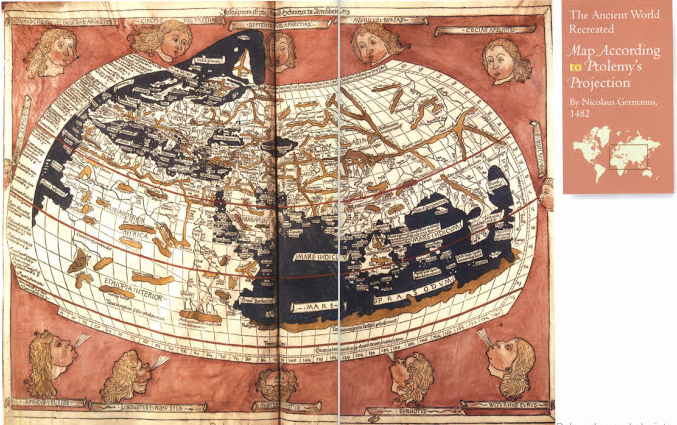
\includegraphics[width=1\textwidth]{figures/PetaPtolemy.PNG}}
	\caption{Gambar Peta menurut Ptolemy}
	\label{PetaPtolemy}
	\end{figure}
	Gambar \ref {PetaPtolemy} Berikut adalah gambar dari Peta yang dibuat oleh Claudius Ptolemy.
	Claudius Ptolemaues yang dikenal dengan nama Ptolemy, hidup antara tahun 100 M dan 168 M, beliau merupakan salah satu sarjana sains pada masanya. Dia tinggal dan bekerja di Alexandria, kota Mesir yang merupakan pusat Intelektual dunia barat dengan perpustakaan paling luas yang pernah diciptakan. Ptolemy membawa semua pengetahuan dan keterampilan matematika dan astronomi dan menerapkannya pada pembuatan peta. Dia memiliki daya tarik matematikawan dengan presisi untuk menunjukkan hubungan satu tempat ke tenpat lain. Berdasarkan perhitungan lingkaran dunia 18.000 mil, ia juga mengembangkan sistem grid latude dan longtude yang dirancang oleh Marinus of Tire. sementara beberapa rincian peta mungkin sedikit aneh dengan garis lintang sejajar dengan garis khatulistiwa dengan garis bujur yang membentang ke utara-selatan dengan busur anggun, sudah tidak asing lagi bagi siapa saja yang pernah memiliki atlas. dalam kerangka ini, ptolemy mampu membangun koordinat dan mendaftarkan lebih dari 8000 tempat dengan koordinat masing-masing. Bagi ptolemy, ini adalah latihan matematik dan kita tidak akan pernah tahu apakah dia benar-benar menggambar peta dari sini.
	Data-data tentang Pembuatan peta sempat hilang ketika perpustakaan Alexandria yang terkenal dibakar oleh orang-orang kristen fanatik pada tahun 390 Masehi - sebuah contoh awal konflik antara iman dan sains. Tapi setidaknya satu salinan yang tealah dibuat dari karya Ptolemy terselamatkan dan ini bertahan di Byzantium. 1000 tahun berlalu dan kemudian tulisannya digunakan untuk dikembangkan oleh ilmuwan Arab, sementara di bagian eropa tetap dalam ketidaktahuan akan warisannya. Baru pada saat renaisans muncul di italia dan daya tarik di dunia, Geografi Ptolemy diterjemahkan dalam bahasa Latin dan gagasannya terhadap PETA Duniadapat diakses oleh para ilmuwan.
	Namun tidak ada peta dalam keadaan masih utuh, hanya petunjuk dan saran untuk pembuatan map dan daftar koordinat.\cite{smart2005maps}
	\begin{figure} [ht]
	\centerline{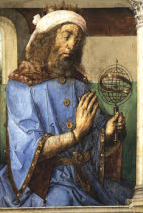
\includegraphics[width=1\textwidth]{figures/ptolemy.PNG}}
	\caption{Foto Ptolemy}
	\label{PetaPtolemy}
	\end{figure}
	gambar \ref{ptolemy} Foto Ptolemy seorang ahli astronomi, geografi, matematikawan.

\subsection{Peta Dunia Ptolemy}
		Peta dunia Ptolemy adalah peta gambaran dunia yang diketahui masyarakat barat pada kurun kedua masihi.Peta tersebut berdasarkan penerangan yang terkandung didalam buku Geographia, ditulis kira-kira pada 150 masihi. walaupun peta autentik tidak dijumpai, buku Geographia yng mengandungi beribu-ribu rujukan pelbagai tempat di dunia lama, berserta kordinat, yang membolehkan para pelukis peta menyusun semula peta dunia Ptolemy apabila manuskriptnya telah ditemui sekitar 1300 masihi.
	\begin{figure} [ht]
	\centerline{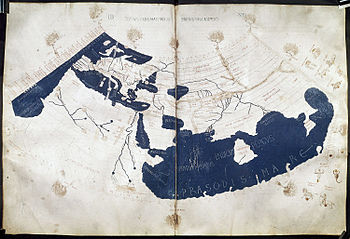
\includegraphics[width=1\textwidth]{figures/PtolemyWorldMap.PNG}}
	\caption{Gambar Ptolemy}	
	\label{PtolemyWorldMap}
	\end{figure}	
	gambar \ref{PetaPtolemy} Peta Dunia Ptolemy, disusun semula dari Geographia Ptolemy (kira-kira 150) pada kurun ke 15, menunjukan ``Sinae" (China) di sebelah kanan, dibawah pulau ``Taprobane" (Sri Lanka, diperbesarkan) dan ``Aurea Chersonesus" (Semenanjung Asia Tenggara).
	\begin{figure} [ht]
	\centerline{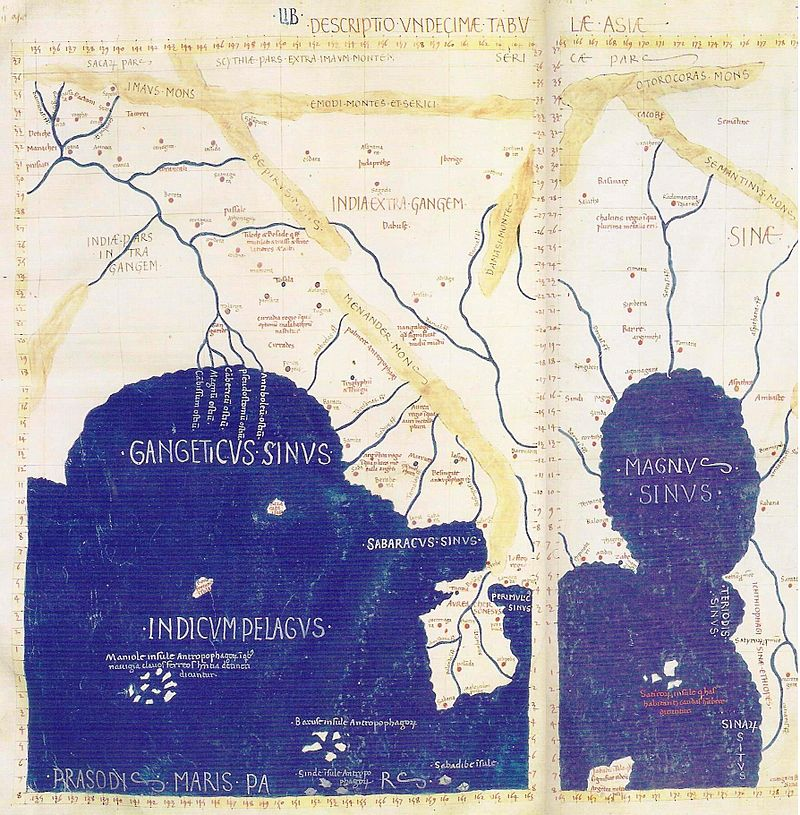
\includegraphics[width=1\textwidth]{figures/PtolemyAsiadetail.PNG}}	
	\caption{Gambar Perincian Timur dan Asia}		
	\end{figure}
	gambar \ref{PtolemyAsiadetail} Perinician Timur dan Asia Tenggara dalam peta dunia Ptolemy.Teluk Ganges (Teluk Bengali) kiri, Semenanjung Asia Tenggara di tengah, Laut China selatan kanan, bersama ``Sinae" (China).
	\subsection{Sejarah ``Ptolemy"}
	\begin{figure} [ht]
	\centerline{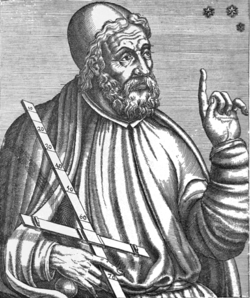
\includegraphics[width=1\textwidth]{figures/Ptolemyporg.PNG}}
	\caption{Konsep artis zaman pertengahan dari Claudius Ptolemaeus.}
	\end{figure}
    gambar \ref{Ptolemyporg}Claudius Ptolemaeus (bahasa Yunani: Κλαύδιος Πτολεμαῖος; 90 – 168), adalah seorang ahli geografi, astronom, dan astrolog yang hidup pada zaman Helenistik di provinsi Romawi, Aegyptus.
    Ptolemaeus adalah pengarang beberapa risalah ilmiah, tiga di antaranya kemudian memainkan peranan penting dalam keilmuwan Islam dan Eropa. Yang pertama adalah risalah astronomi yang dikenal sebagai Almagest (dalam bahasa Yunani Η μεγάλη Σύνταξις , ``Risalah Besar"). Yang kedua adalah Geographia, yang merupakan diskusi teliti mengenai pengetahuan geografi Helenistik. Yang ketiga adalah risalah astrologi dikenal sebagai Tetrabiblos (``Empat buku") di mana dia berusaha mengadaptasi astrologi horoskop ke filosofi alam Aristotelian. Ia juga melestarikan daftar raja-raja kuno, disebut ``Kanon Ptolemaeus", yang penting bagi penelitian sejarah Timur Tengah.
    Claudius adalah nomen (nama keluarga) seorang Roma; Ptolemaeus menyandang nama itu, sehingga menjadi bukti bahwa dia adalah seorang warganegara Roma. Sesuai kebiasaan, Keluarga Ptolemy pertama yang menjadi warganegara (entah itu dia atau nenek moyangnya) mengambil nama itu dari seorang Roma yang bernama Claudius, sehingga membuatnya diberi status kewarganegaraan. Jika orang Roma ini adalah kaisar, kewarganegaraan sudah akan diberi di antara tahun 41 dan 68 M. (waktu Claudius, lalu Nero, menjabat kaisar). Astronom itu juga mempunyai praenomen (nama pertama), yang tetap tak diketahui. Tetapi, kemungkinan Tiberius, karena praenomen itu sangat umum di antara yang keluarga-keluarga yang diberi kewarganegaraan oleh kaisar ini.
    Ptolemaeus (Ptolemy) adalah sebuah nama Yunani. Muncul satu kali di mitologi Yunani, dalam bentuk Homeric. Cukup biasa di antara golongan sol bagian atas Makedonia pada saat Alexander Agung, dan ada beberapa di antara tentara Alexander, satu di antaranya pada tahun 323 S.M. menjadikan dirinya sendiri Raja Mesir: Ptolemy I Soter; semua raja setelah dia, sampai Mesir menjadi provinsi Roma pada tahun 30 S.M., adalah juga dari dinasti Ptolemaic. Hanya ada sedikit bukti tentang subyek asal usul Ptolemy (meskipun melihat di atas kewarganegaraan Roma keluarganya), tetapi kebanyakan sarjana dan sejarawan mempertimbangkannya tak mungkin bahwa Ptolemeus berhubungan dengan dinasti kerajaan Ptolemies.
    Selain dianggap sebagai seorang anggota masyarakat Yunani Alexandria, hanya sedikit rincian hidup Ptolemaeus yang diketahui. Dia menulis dalam bahasa Yunani Kuno dan diketahui sudah menggunakan data astronomis Babilonia.Seorang warganegara Roma, beberapa sarjana menyimpulkan bahwa secara etnik, Ptolemeus adalah orang Yunani, dan sarjana lainnya berpendapat bahwa dia secara etnik orang Mesir, meskipun Hellenize. Dia banyak dikenal dalam sumber bahasa Arab yang muncul kemudian sebagai Upper Egyptian, diperkirakan dia mungkin berasal dari Mesir selatan. Astronom, ahli ilmu bumi, dan pakar fisika Arab selanjutnya merujuk padanya menggunakan nama Arabnya Batlamyus.
    Karya utama Ptolemy lainnya adalah Geografinya (juga disebut Geographia), kompilasi koordinat geografis dari bagian dunia yang dikenal oleh Kekaisaran Romawi pada masanya. Dia agak bergantung pada karya seorang ahli geografi sebelumnya, Marinos of Tire, dan pada kano Romawi dan Kekaisaran Persia kuno. [Rujukan?] Dia juga mengakui astronom Hipparchus kuno karena telah menyediakan ketinggian kutub utara untuk beberapa kota. [19]
   
\subsection{The Geography}	
   \begin{figure} [ht]
	\centerline{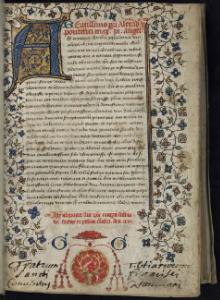
\includegraphics[width=1\textwidth]{figures/geography.PNG}}
	\caption{Geography by Ptolemy.}
		\end{figure}
    gambar \ref{geography} Bagian pertama dari Geografi adalah diskusi tentang data dan metode yang dia gunakan. Seperti model tata surya di Almagest, Ptolemy memasukkan semua informasi ini ke dalam skema besar. Setelah Marinos, dia memberikan koordinat ke semua tempat dan fitur geografis yang dia ketahui, dalam kotak yang membentang di seluruh dunia. Lintang diukur dari khatulistiwa, seperti sekarang, tapi Ptolemy lebih suka [20] untuk mengekspresikannya sebagai climata, panjang hari terpanjang daripada deretan busur: panjang hari senin mulai meningkat dari 12h menjadi 24 jam saat seseorang pergi. dari khatulistiwa ke lingkaran kutub. Dalam buku 2 sampai 7, dia menggunakan gelar dan meletakkan garis meridian 0 bujur di tanah paling barat yang dia kenal, ``Kepulauan Terberkati", yang sering diidentifikasi sebagai Kepulauan Canary, seperti yang disarankan oleh lokasi dari enam titik yang diberi label ``FORTUNATA" pulau-pulau di dekat ekstrem kiri laut biru peta Ptolemeus di sini direproduksi.
	Ptolemeus juga merancang dan memberikan petunjuk bagaimana membuat peta di seluruh dunia yang berpenghuni (oikoumenè) dan provinsi Romawi. Di bagian kedua Geografi, dia memberikan daftar topografi yang diperlukan, dan teks untuk peta. Oikoumenènya membentang 180 derajat bujur dari Kepulauan Terberkati di Samudra Atlantik sampai ke Cina tengah, dan sekitar 80 derajat garis lintang dari Shetland menjadi anti-Meroe (pantai timur Afrika); Ptolemy sangat sadar bahwa dia tahu tentang hanya seperempat dunia, dan perpanjangan yang salah dari Cina ke selatan menunjukkan sumbernya tidak sampai ke Samudra Pasifik.
	Peta di manuskrip yang masih ada di Ptolemy's Geography, bagaimanapun, hanya berasal dari sekitar tahun 1300, setelah teks tersebut ditemukan kembali oleh Maximus Planudes. Tampaknya tabel topografi dalam buku 2-7 adalah teks kumulatif - teks yang diubah dan ditambahkan sebagai pengetahuan baru yang tersedia di abad setelah Ptolemy. [21] Ini berarti bahwa informasi yang terdapat di berbagai bagian Geografi kemungkinan berasal dari tanggal yang berbeda. 
	Peta berdasarkan prinsip ilmiah telah dibuat sejak zaman Eratosthenes, pada abad ke-3 SM, namun Ptolemy memperbaiki proyeksi peta. Diketahui dari sebuah pidato oleh Eumenius bahwa peta dunia, sebuah orbis pictus, yang tidak diragukan lagi berdasarkan Geografi, dipajang di sebuah sekolah di Augustodunum, Gaul pada abad ketiga. [22] Pada abad ke-15, Geografi Ptolemy mulai dicetak dengan peta terukir; edisi cetak paling awal dengan peta terukir diproduksi di Bologna pada 1477, diikuti dengan cepat oleh edisi Romawi tahun 1478 (Campbell, 1987). Sebuah edisi yang dicetak di Ulm pada tahun 1482, termasuk peta tebing kayu, adalah yang pertama dicetak di utara Pegunungan Alpen. Peta terlihat terdistorsi bila dibandingkan dengan peta modern, karena data Ptolemy tidak akurat. Salah satu alasannya adalah Ptolemy memperkirakan ukuran Bumi terlalu kecil: sementara Eratosthenes menemukan 700 stadion untuk sebuah lingkaran besar di dunia, Ptolemy menggunakan 500 stadion di Geografi. Sangat mungkin bahwa ini adalah stadion yang sama, karena Ptolemy beralih dari skala sebelumnya ke yang terakhir antara Syntaxis dan Geography, dan menyesuaikan derajat bujur yang sesuai. Lihat juga unit pengukuran dan Sejarah Yunani Kuno geodesi.
	Karena Ptolemy berasal dari garis lintang utamanya dari nilai terpanjang minyak mentah, garis lintangnya rata-rata keliru kira-kira satu derajat (2 derajat untuk Bizantium, 4 derajat untuk Kartago), meskipun para astronom kuno mampu mengetahui garis lintang mereka lebih lama. (Lambang Ptolemeus sendiri salah oleh 14 '.) Dia setuju (Geografi 1.4) bahwa bujur paling baik ditentukan oleh observasi simultan gerhana bulan, namun dia sangat tidak berhubungan dengan ilmuwan pada masanya bahwa dia tidak mengetahui data semacam itu. lebih baru dari 500 tahun sebelumnya (Arbela gerhana). Ketika beralih dari 700 stadia per derajat ke 500, dia (atau Marinos) memperluas perbedaan bujur antara kota-kota yang sesuai (sebuah titik yang pertama kali direalisasikan oleh P.Gosselin pada tahun 1790), yang mengakibatkan peregangan skala bumi timur-barat yang serius dalam derajat, meski tidak jauh. Mencapai garis bujur yang sangat tepat tetap menjadi masalah dalam geografi sampai penerapan metode bulan Jovian Galileo di abad ke-18. Harus ditambahkan bahwa daftar topografinya yang asli tidak dapat direkonstruksi: tabel panjang dengan angka dikirim ke anak cucu melalui salinan yang mengandung banyak kesalahan juru tulis, dan orang selalu menambahkan atau memperbaiki data topografi: ini adalah kesaksian akan popularitas yang terus-menerus dari Karya ini berpengaruh dalam sejarah kartografi.
	}
=======
%kelompok 2 GIS (Ptolemy)
%Tiara Rizki Wulansari (1154026)
% Muhamad Rifan Zamaludin (1154088)
% Mohammad Agung Deomartha (1154032)
% M. Fajri Mualim (1154078)
% Faisal Syarifuddin

\section{Peta}
	peta adalah/merupakan penggambaran secara grafis atau bentuk skala (perbandingan) pada konsep mengenai bumi. dalam hal ini peta merupakan alat untuk menyampaikan atau menginformasikan mengenai ilmu kebumian. bagaimana peta dahulu ditemukan ? pengetahuan mengenai dasar pembentukan peta sama seperti filosofi, yang mana sering terdapat perbedaan.

\subsection{Peta Menurut Claudius Ptolemaeus Ptolemy}
	\begin{figure} [ht]
	\centerline{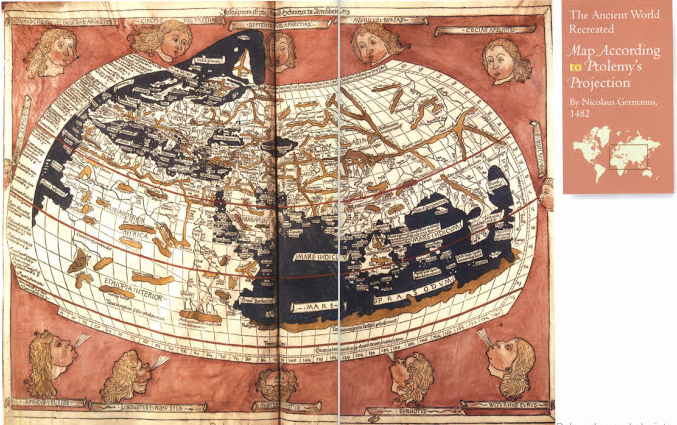
\includegraphics[width=1\textwidth]{figures/PetaPtolemy.PNG}}
	\caption{Gambar Peta menurut Ptolemy}
	\label{PetaPtolemy}
	\end{figure}
	Gambar \ref {PetaPtolemy} Berikut adalah gambar dari Peta yang dibuat oleh Claudius Ptolemy.
	Claudius Ptolemaues yang dikenal dengan nama Ptolemy, hidup antara tahun 100 M dan 168 M, beliau merupakan salah satu sarjana sains pada masanya. Dia tinggal dan bekerja di Alexandria, kota Mesir yang merupakan pusat Intelektual dunia barat dengan perpustakaan paling luas yang pernah diciptakan. Ptolemy membawa semua pengetahuan dan keterampilan matematika dan astronomi dan menerapkannya pada pembuatan peta. Dia memiliki daya tarik matematikawan dengan presisi untuk menunjukkan hubungan satu tempat ke tenpat lain. Berdasarkan perhitungan lingkaran dunia 18.000 mil, ia juga mengembangkan sistem grid latude dan longtude yang dirancang oleh Marinus of Tire. sementara beberapa rincian peta mungkin sedikit aneh dengan garis lintang sejajar dengan garis khatulistiwa dengan garis bujur yang membentang ke utara-selatan dengan busur anggun, sudah tidak asing lagi bagi siapa saja yang pernah memiliki atlas. dalam kerangka ini, ptolemy mampu membangun koordinat dan mendaftarkan lebih dari 8000 tempat dengan koordinat masing-masing. Bagi ptolemy, ini adalah latihan matematik dan kita tidak akan pernah tahu apakah dia benar-benar menggambar peta dari sini.
	Data-data tentang Pembuatan peta sempat hilang ketika perpustakaan Alexandria yang terkenal dibakar oleh orang-orang kristen fanatik pada tahun 390 Masehi - sebuah contoh awal konflik antara iman dan sains. Tapi setidaknya satu salinan yang tealah dibuat dari karya Ptolemy terselamatkan dan ini bertahan di Byzantium. 1000 tahun berlalu dan kemudian tulisannya digunakan untuk dikembangkan oleh ilmuwan Arab, sementara di bagian eropa tetap dalam ketidaktahuan akan warisannya. Baru pada saat renaisans muncul di italia dan daya tarik di dunia, Geografi Ptolemy diterjemahkan dalam bahasa Latin dan gagasannya terhadap PETA Duniadapat diakses oleh para ilmuwan.
	Namun tidak ada peta dalam keadaan masih utuh, hanya petunjuk dan saran untuk pembuatan map dan daftar koordinat \cite{smart2005maps}.
	\begin{figure} [ht]
	\centerline{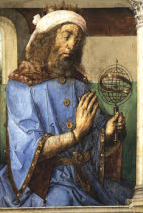
\includegraphics[width=1\textwidth]{figures/ptolemy.PNG}}
	\caption{Foto Ptolemy}
	\label{ptolemy}
	\end{figure}
	gambar \ref{ptolemy} Foto Ptolemy seorang ahli astronomi, geografi, matematikawan.

\subsection{Peta Dunia Ptolemy}
		Peta dunia Ptolemy adalah peta gambaran dunia yang diketahui masyarakat barat pada kurun kedua masihi.Peta tersebut berdasarkan penerangan yang terkandung didalam buku Geographia, ditulis kira-kira pada 150 masihi. walaupun peta autentik tidak dijumpai, buku Geographia yng mengandungi beribu-ribu rujukan pelbagai tempat di dunia lama, berserta kordinat, yang membolehkan para pelukis peta menyusun semula peta dunia Ptolemy apabila manuskriptnya telah ditemui sekitar 1300 masihi.
	\begin{figure} [ht]
	\centerline{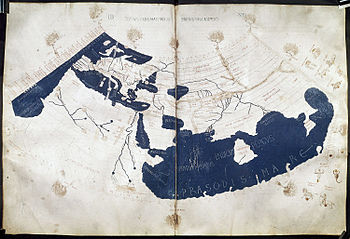
\includegraphics[width=1\textwidth]{figures/PtolemyWorldMap.PNG}}
	\caption{Gambar Ptolemy}	
	\label{PtolemyWorldMap}
	\end{figure}
	gambar \ref {PtolemyWorldMap} Peta Dunia Ptolemy, disusun semula dari Geographia Ptolemy (kira-kira 150) pada kurun ke 15, menunjukan Sinae (China) di sebelah kanan, dibawah pulau Taprobane (Sri Lanka, diperbesarkan) dan Aurea Chersonesus (Semenanjung Asia Tenggara).

	\begin{figure} [ht]
	\centerline{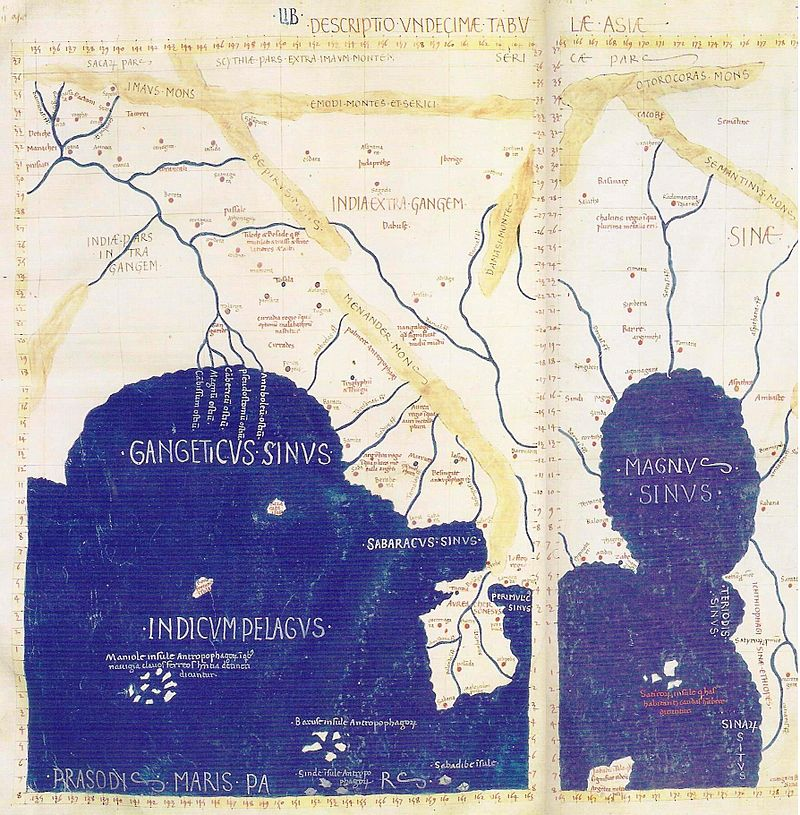
\includegraphics[width=1\textwidth]{figures/PtolemyAsiadetail.PNG}}	
	\caption{Gambar Perincian Timur dan Asia}
	\label{PtolemyAsiadetail}		
	\end{figure}
	gambar \ref{PtolemyAsiadetail} Perinician Timur dan Asia Tenggara dalam peta dunia Ptolemy.Teluk Ganges (Teluk Bengali) kiri, Semenanjung Asia Tenggara di tengah, Laut China selatan kanan, bersama Sinae (China).
	
\subsection{Sejarah Ptolemy}
	\begin{figure} [ht]
	\centerline{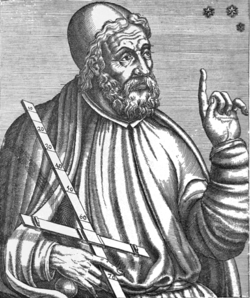
\includegraphics[width=1\textwidth]{figures/Ptolemyporg.PNG}}
	\caption{Konsep artis zaman pertengahan dari Claudius Ptolemaeus.}
	\label{Ptolemyporg}
	\end{figure}
    gambar \ref{Ptolemyporg} Claudius Ptolemaeus (bahasa Yunani: Κλαύδιος Πτολεμαῖος; 90 – 168), adalah seorang ahli geografi, astronom, dan astrolog yang hidup pada zaman Helenistik di provinsi Romawi, Aegyptus.
    Ptolemaeus adalah pengarang beberapa risalah ilmiah, tiga di antaranya kemudian memainkan peranan penting dalam keilmuwan Islam dan Eropa. Yang pertama adalah risalah astronomi yang dikenal sebagai Almagest (dalam bahasa Yunani Η μεγάλη Σύνταξις , Risalah Besar). Yang kedua adalah Geographia, yang merupakan diskusi teliti mengenai pengetahuan geografi Helenistik. Yang ketiga adalah risalah astrologi dikenal sebagai Tetrabiblos (Empat buku) di mana dia berusaha mengadaptasi astrologi horoskop ke filosofi alam Aristotelian. Ia juga melestarikan daftar raja-raja kuno, disebut Kanon Ptolemaeus, yang penting bagi penelitian sejarah Timur Tengah.
    Claudius adalah nomen (nama keluarga) seorang Roma; Ptolemaeus menyandang nama itu, sehingga menjadi bukti bahwa dia adalah seorang warganegara Roma. Sesuai kebiasaan, Keluarga Ptolemy pertama yang menjadi warganegara (entah itu dia atau nenek moyangnya) mengambil nama itu dari seorang Roma yang bernama Claudius, sehingga membuatnya diberi status kewarganegaraan. Jika orang Roma ini adalah kaisar, kewarganegaraan sudah akan diberi di antara tahun 41 dan 68 M. (waktu Claudius, lalu Nero, menjabat kaisar). Astronom itu juga mempunyai praenomen (nama pertama), yang tetap tak diketahui. Tetapi, kemungkinan Tiberius, karena praenomen itu sangat umum di antara yang keluarga-keluarga yang diberi kewarganegaraan oleh kaisar ini.
    Ptolemaeus (Ptolemy) adalah sebuah nama Yunani. Muncul satu kali di mitologi Yunani, dalam bentuk Homeric. Cukup biasa di antara golongan sol bagian atas Makedonia pada saat Alexander Agung, dan ada beberapa di antara tentara Alexander, satu di antaranya pada tahun 323 S.M. menjadikan dirinya sendiri Raja Mesir: Ptolemy I Soter; semua raja setelah dia, sampai Mesir menjadi provinsi Roma pada tahun 30 S.M., adalah juga dari dinasti Ptolemaic. Hanya ada sedikit bukti tentang subyek asal usul Ptolemy (meskipun melihat di atas kewarganegaraan Roma keluarganya), tetapi kebanyakan sarjana dan sejarawan mempertimbangkannya tak mungkin bahwa Ptolemeus berhubungan dengan dinasti kerajaan Ptolemies.
    Selain dianggap sebagai seorang anggota masyarakat Yunani Alexandria, hanya sedikit rincian hidup Ptolemaeus yang diketahui. Dia menulis dalam bahasa Yunani Kuno dan diketahui sudah menggunakan data astronomis Babilonia.Seorang warganegara Roma, beberapa sarjana menyimpulkan bahwa secara etnik, Ptolemeus adalah orang Yunani, dan sarjana lainnya berpendapat bahwa dia secara etnik orang Mesir, meskipun Hellenize. Dia banyak dikenal dalam sumber bahasa Arab yang muncul kemudian sebagai Upper Egyptian, diperkirakan dia mungkin berasal dari Mesir selatan. Astronom, ahli ilmu bumi, dan pakar fisika Arab selanjutnya merujuk padanya menggunakan nama Arabnya Batlamyus.
    Karya utama Ptolemy lainnya adalah Geografinya (juga disebut Geographia), kompilasi koordinat geografis dari bagian dunia yang dikenal oleh Kekaisaran Romawi pada masanya. Dia agak bergantung pada karya seorang ahli geografi sebelumnya, Marinos of Tire, dan pada kano Romawi dan Kekaisaran Persia kuno. [Rujukan] Dia juga mengakui astronom Hipparchus kuno karena telah menyediakan ketinggian kutub utara untuk beberapa kota.[19]
  
  \subsection{The Geography}	
   \begin{figure} [ht]
	\centerline{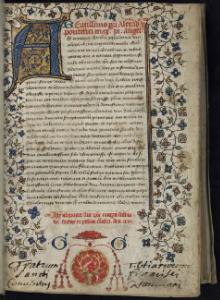
\includegraphics[width=1\textwidth]{figures/geography.PNG}}
	\caption{Geography by Ptolemy.}
	\label{geography}
		\end{figure}
    gambar \ref {geography} Bagian pertama dari Geografi adalah diskusi tentang data dan metode yang dia gunakan. Seperti model tata surya di Almagest, Ptolemy memasukkan semua informasi ini ke dalam skema besar. Setelah Marinos, dia memberikan koordinat ke semua tempat dan fitur geografis yang dia ketahui, dalam kotak yang membentang di seluruh dunia. Lintang diukur dari khatulistiwa, seperti sekarang, tapi Ptolemy lebih suka [20] untuk mengekspresikannya sebagai climata, panjang hari terpanjang daripada deretan busur: panjang hari senin mulai meningkat dari 12h menjadi 24 jam saat seseorang pergi. dari khatulistiwa ke lingkaran kutub. Dalam buku 2 sampai 7, dia menggunakan gelar dan meletakkan garis meridian 0 bujur di tanah paling barat yang dia kenal, Kepulauan Terberkati, yang sering diidentifikasi sebagai Kepulauan Canary, seperti yang disarankan oleh lokasi dari enam titik yang diberi label FORTUNATA pulau-pulau di dekat ekstrem kiri laut biru peta Ptolemeus di sini direproduksi.
	Ptolemeus juga merancang dan memberikan petunjuk bagaimana membuat peta di seluruh dunia yang berpenghuni (oikoumenè) dan provinsi Romawi. Di bagian kedua Geografi, dia memberikan daftar topografi yang diperlukan, dan teks untuk peta. Oikoumenènya membentang 180 derajat bujur dari Kepulauan Terberkati di Samudra Atlantik sampai ke Cina tengah, dan sekitar 80 derajat garis lintang dari Shetland menjadi anti-Meroe (pantai timur Afrika); Ptolemy sangat sadar bahwa dia tahu tentang hanya seperempat dunia, dan perpanjangan yang salah dari Cina ke selatan menunjukkan sumbernya tidak sampai ke Samudra Pasifik.
	Peta di manuskrip yang masih ada di Ptolemy's Geography, bagaimanapun, hanya berasal dari sekitar tahun 1300, setelah teks tersebut ditemukan kembali oleh Maximus Planudes. Tampaknya tabel topografi dalam buku 2-7 adalah teks kumulatif - teks yang diubah dan ditambahkan sebagai pengetahuan baru yang tersedia di abad setelah Ptolemy. [21] Ini berarti bahwa informasi yang terdapat di berbagai bagian Geografi kemungkinan berasal dari tanggal yang berbeda. 
	Peta berdasarkan prinsip ilmiah telah dibuat sejak zaman Eratosthenes, pada abad ke-3 SM, namun Ptolemy memperbaiki proyeksi peta. Diketahui dari sebuah pidato oleh Eumenius bahwa peta dunia, sebuah orbis pictus, yang tidak diragukan lagi berdasarkan Geografi, dipajang di sebuah sekolah di Augustodunum, Gaul pada abad ketiga. [22] Pada abad ke-15, Geografi Ptolemy mulai dicetak dengan peta terukir; edisi cetak paling awal dengan peta terukir diproduksi di Bologna pada 1477, diikuti dengan cepat oleh edisi Romawi tahun 1478 (Campbell, 1987). Sebuah edisi yang dicetak di Ulm pada tahun 1482, termasuk peta tebing kayu, adalah yang pertama dicetak di utara Pegunungan Alpen. Peta terlihat terdistorsi bila dibandingkan dengan peta modern, karena data Ptolemy tidak akurat. Salah satu alasannya adalah Ptolemy memperkirakan ukuran Bumi terlalu kecil: sementara Eratosthenes menemukan 700 stadion untuk sebuah lingkaran besar di dunia, Ptolemy menggunakan 500 stadion di Geografi. Sangat mungkin bahwa ini adalah stadion yang sama, karena Ptolemy beralih dari skala sebelumnya ke yang terakhir antara Syntaxis dan Geography, dan menyesuaikan derajat bujur yang sesuai. Lihat juga unit pengukuran dan Sejarah Yunani Kuno geodesi.
	Karena Ptolemy berasal dari garis lintang utamanya dari nilai terpanjang minyak mentah, garis lintangnya rata-rata keliru kira-kira satu derajat (2 derajat untuk Bizantium, 4 derajat untuk Kartago), meskipun para astronom kuno mampu mengetahui garis lintang mereka lebih lama. (Lambang Ptolemeus sendiri salah oleh 14.) Dia setuju (Geografi 1.4) bahwa bujur paling baik ditentukan oleh observasi simultan gerhana bulan, namun dia sangat tidak berhubungan dengan ilmuwan pada masanya bahwa dia tidak mengetahui data semacam itu. lebih baru dari 500 tahun sebelumnya (Arbela gerhana). Ketika beralih dari 700 stadia per derajat ke 500, dia (atau Marinos) memperluas perbedaan bujur antara kota-kota yang sesuai (sebuah titik yang pertama kali direalisasikan oleh P.Gosselin pada tahun 1790), yang mengakibatkan peregangan skala bumi timur-barat yang serius dalam derajat, meski tidak jauh. Mencapai garis bujur yang sangat tepat tetap menjadi masalah dalam geografi sampai penerapan metode bulan Jovian Galileo di abad ke-18. Harus ditambahkan bahwa daftar topografinya yang asli tidak dapat direkonstruksi: tabel panjang dengan angka dikirim ke anak cucu melalui salinan yang mengandung banyak kesalahan juru tulis, dan orang selalu menambahkan atau memperbaiki data topografi: ini adalah kesaksian akan popularitas yang terus-menerus dari Karya ini berpengaruh dalam sejarah kartografi.
	
>>>>>>> 6a8108a428c212f725996110cef23fc85d44868e



%\chapter[Sejarah aliddrissi]
%{Pendahuluan\\ aliddrissi}
%% Kelompok 3
% Ajrina Dharman (1154079)
% Diana Satima G (1154018)
% Indah Rahmawati (1154070)
% M. Amran Hakim Siregar (1154106)
% Rizky Abdul Ghani Suherli (1154048)

\section{Peta}
	peta adalah/merupakan penggambaran secara grafis atau bentuk skala (perbandingan) pada konsep mengenai bumi. dalam hal ini peta merupakan alat untuk menyampaikan atau menginformasikan mengenai ilmu kebumian. bagaimana peta dahulu ditemukan ? pengetahuan mengenai dasar pembentukan peta sama seperti filosofi, yang mana sering terdapat perbedaan.

\subsection{Peta Menurut Abu Abdullah Muhammad al-Idrisi al-Qurtubi al-Hasani as-Sabti "al-Idrisi"}
	\begin{figure} [ht]
	\centerline{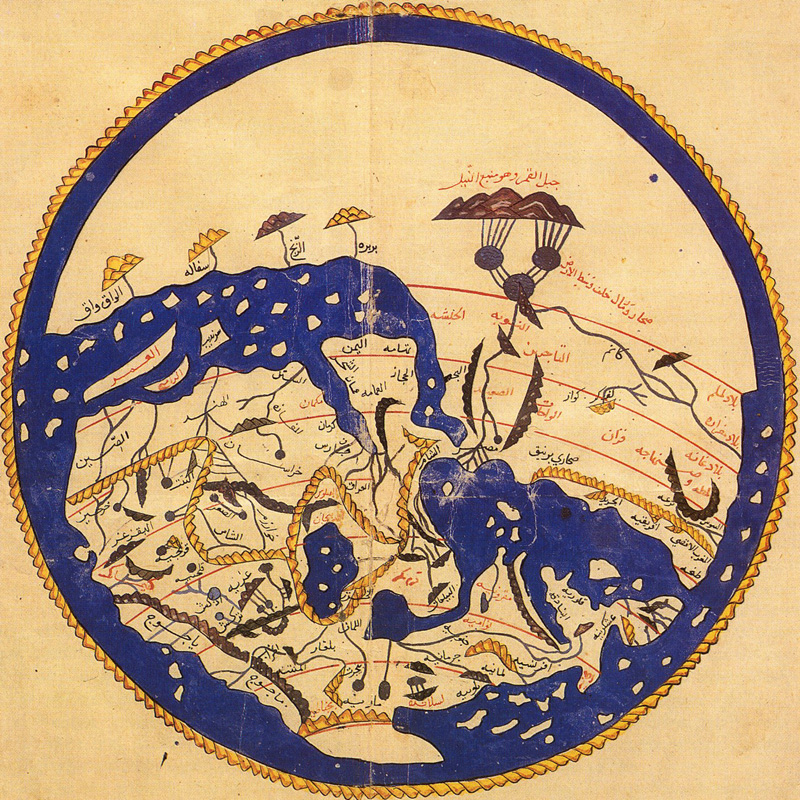
\includegraphics[width=1\textwidth]{figures/1.jpg}}
	\caption{Gambar Peta menurut al-Idrisi}
	\label{Petaal-Idrisi}
	\end{figure}
	\ref{1.jpg} Berikut adalah gambar dari Peta yang dibuat oleh Muhammad al - Idrisi.
	Abu Abdullah Muhammad al-Idrisi al-Qurtubi al-Hasani as-Sabti yang dikenal dengan nama al-Idrisi, hidup antara tahun 1100 – 1165. Al-Idrisi lahir di keluarga Hammudid besar Afrika Utara dan Al-Andalus, yang mengklaim turun dari Idrisids of Morocco dan akhirnya nabi Muhammad. Al-Idrisi lahir di kota Ceuta, di mana kakek buyutnya terpaksa menetap setelah jatuhnya Hammudid Málaga ke Zirids di Granada. Dia menghabiskan sebagian besar masa mudanya untuk bepergian melalui Afrika Utara dan Al-Andalus (Spanyol Muslim saat ini) dan tampaknya telah mendapatkan informasi terperinci mengenai kedua wilayah tersebut. Dia mengunjungi Anatolia saat dia baru berusia 16 tahun. Dia belajar di Córdoba.
	Al-Idrisi memasukkan pengetahuan tentang Afrika, Samudera Hindia dan Timur Jauh yang dikumpulkan oleh pedagang dan penjelajah Islam dan dicatat di peta Islam dengan informasi yang dibawa oleh pelayaran Norman untuk membuat peta dunia yang paling akurat pada zaman pra-modern, yang berfungsi sebagai ilustrasi konkret Kitab nuzhat al-mushtaq-nya, yang dapat diterjemahkan sebagai Pengalihan Manusia untuk Berkelana ke Tempat yang Jauh. 
	Tabula Rogeriana digambar oleh Al-Idrisi pada tahun 1154 untuk Raja Norman Roger II dari Sisilia, setelah tinggal delapan belas tahun di istananya, di mana dia mengerjakan komentar dan ilustrasi peta. Peta tersebut, dengan legenda yang ditulis dalam bahasa Arab, sekaligus menunjukkan benua Eurasia secara keseluruhan, hanya menunjukkan bagian utara benua Afrika dan tidak memiliki rincian Tanduk Afrika dan Asia Tenggara.
	\ref{3.jpg} Berikut adalah gambar dari Peta Tabula Rogeriana digambar oleh Al-Idrisi.
	\begin{figure} [ht]
	\centerline{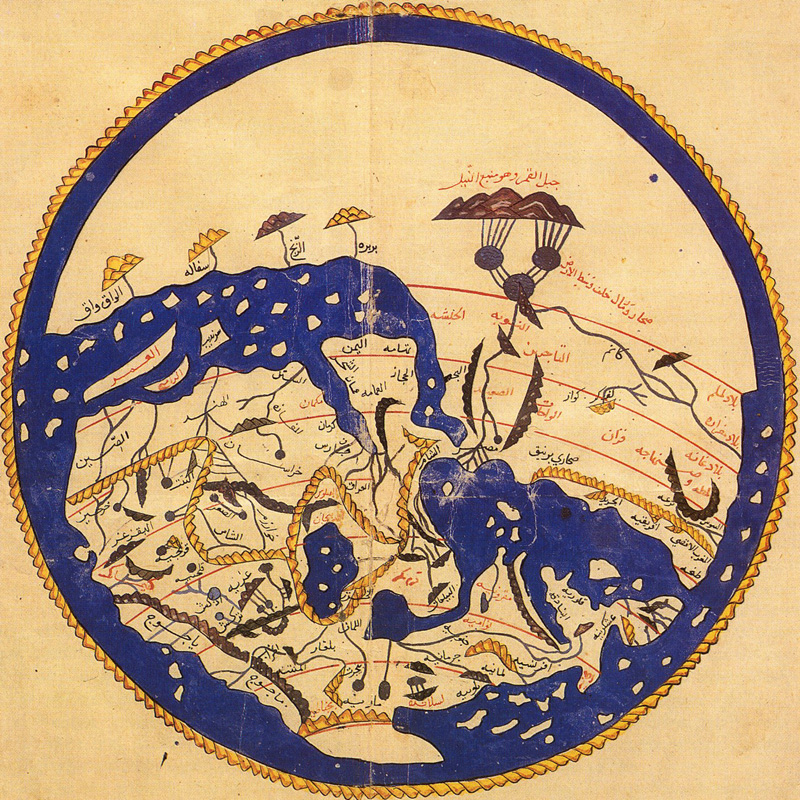
\includegraphics[width=1\textwidth]{figures/1.jpg}}
	\caption{Foto al-Idrisi}
	\end{figure}
	\ref{2.jpg} Foto al-Idrisi seorang ahli geografi,.
	

\subsection {Sejarah Peta dari pandangan Al-Qur'an "al-idrisi"}
	Pandangan Islam mempercayai adanya dua keghaiban, yaitu keghaiban yang eksistensinya tidak harus terukur atau tidak harus difahami melalui metodologi sains, keghaiban yang difahami melalui sistem keimanan, selain itu juga keghaiban yang dikenal sebagai sunattullah. Manusia tak menyaksikan secara langsung tentang proses-proses pembentukan alamsemesta, bahkan kehidupannya di planit Bumi ini hanya merupakan sebagian kecil episode dalam alamsemesta.
	Metodologi sains, Islam memperkenalkan sebuah metodologi lain yaitu ilmupengetahuan (tentang eksistensi kebenaran) bagi manusia bisa bersumber dari sumber terpercaya (kitab Allah) dan disampaikan dengan cara terpercaya. Al Qur’an merupakan sebuah kebenaran yang melengkapi pandangan yang dibangun melalui rasionalitas manusia semata, memperkenalkan Allah sebagai Tuhan alam semesta, ada alam ghaib, ada sesuatu yang ghaib dan manusia tak banyak mengetahuinya, ada cara atau upaya-upaya mencapai atau berkomunikasi dengan Yang MahaPencipta dan MahaPenguasa alam semesta. Pemahaman sunatullah dipergunakan untuk penyempurnaan dan membuat kemudahan-kemudahan dalam hidup dan beribadah agar bisa senantiasa lebih mendekat lagi kepada Allah swt, MahaPencipta dan MahaPenguasa alam semesta.
	Al Qur’an sebagai wahyu Allah yang telah diturunkan kepada umat manusia, perlu dipandang sebagai “resources” bagi kehidupan umat manusia di planit Bumi yaitu sebagai petunjuk Allah swt agar hati manusia bisa tertuntun dan terdidik sehingga berahlak mulia. Gambaran wahyu Allah dalam al Qur'an mengingatkan walaupun ada kepastian dari “tangan-tangan ghaib berupa sunatullah” yang sebagian telah bisa diungkap melalui metodologi sains, namun masih terdapat pengetahuan dan kehendakNya yang ghaib dalam penciptaan Alam Semesta. 
	Pemikiran atas fenomena alam semesta itu sangat diharapkan bisa membangun kesadaran beragama, mempertemukan “kerja tangan-tangan ghaib Allah” yang mengatur alam semesta dengan wahyuNya dalam al Qur’an. Keduanya adalah kebenaran yang berasal dari yang Allah zat yang Maha Esa. Mempertemukan kebenaran wahyu Allah dan ayat kauniyah merupakan proses pemahaman manusia tentang lingkungan kehidupannya yang lebih luas, menjangkau dunia dan akherat, memadukan akal dan keyakinan dalam perspektif Islam. 
	Abad sains dan teknologi telah dijalani manusia, makin tinggi pengetahuan manusia makin diperlukan kesadaran beragama yang lebih tinggi, perlu hidayah yang lebih banyak, agar mendapatkan tuntunanNya sehingga dijauhkan dari bencana sains dan teknologi. 
	Berbagai bentuk upaya-upaya dakwah umat Islam perlu dikembangkan, upaya dakwah hendaknya juga menggerakkan kaum muda masyarakat kampus maupun non kampus dengan wawasan membangun kualitas lingkungan. Agar peran umat Islam dalam hal amar ma’ruf nahi munkar dapat lebih dirasakan dalam masyarakat, perlu dirancang kegiatan yang bersinambung dalam pengembangan, pembelajaran maupun sosialisasi IPTEK. 
	Di abad ke-11 M, seorang geografer termasyhur dari Spanyol, Abu Ubaid Al Bakri berhasil menulis kitab di bidang geografi, yakni Mu’jam Al Ista’jam (Ensiklopedi Geografi) dan Al Masalik wa Al Mamalik (Jalan dan Kerajaan). Buku pertama berisi nama-nama tempat di Jazirah Arab. Sedangkan yang kedua berisi pemetaan geografis dunia Arab zaman dahulu.
	Pada abad ke-12, geografer Muslim Al Idrisi berhasil membuat peta dunia. Al Idrisi yang lahir pada tahun 1100 di Ceuta Spanyol itu juga menulis kitab geografi berjudul Kitab Nazhah Al Muslak fi Ikhtira Al Falak (Tempat Orang yang Rindu Menembus Cakrawala). Kitab ini begitu berpengaruh sehingga diterjemahkan ke dalam bahasa Latin, Geographia Nubiensis.
	Seabad kemudian, dua geografer Muslim yakni Qutubuddin Asy Syirazi (1236 M-1311 M) dan Yaqut Ar Rumi (1179 M-1229 M) berhasil melakukan terobosan baru. Qutubuddin mampu membuat peta Laut Putih atau Laut Tengah yang dihadiahkan kepada Raja Persia. Sedangkan, Yaqut berhasil menulis enam jilid ensiklopedi bertajuk Mu’jam Al Buldan (Ensiklopedi Negeri-negeri).
	Penjelajah Muslim asal Maroko, Ibnu Battutah di abad ke-14 M memberi sumbangan dalam menemukan rute perjalanan baru. Hampir selama 30 tahun, Ibnu Battutah menjelajahi daratan dan mengarungi lautan untuk berkeliling dunia. Penjelajah Muslim lainnya yang mampu mengubah rute perjalanan laut adalah Laksamana Cheng Ho dari Tiongkok. Dia melakukan ekspedisi sebanyak tujuh kali mulai dari tahun 1405 hingga 1433 M.
	Sederet geografer Muslim telah banyak memberi kontribusi bagi pengembangan ilmu bumi. Al Kindi diakui begitu berjasa sebagai geografer pertama yang memperkenalkan percobaan ke dalam ilmu bumi. Sedangkan, Al Biruni didapuk sebagai “bapak geodesi” yang banyak memberi kontribusi terhadap geografi dan juga geologi.
	John J O’Connor dan Edmund F Robertson menuliskan pengakuannya terhadap kontribusi Al Biruni dalam MacTutor History of Mathematics. Menurut mereka, “Al Biruni telah menyumbangkan kontribusi penting bagi pengembangan geografi dan geodesi. Dialah yang memperkenalkan teknik pengukuran bumi dan jaraknya dengan menggunakan triangulation”.
	Al Birunilah yang menemukan radius bumi mencapai 6.339,6 km. Hingga abad ke-16 M, Barat belum mampu mengukur radius bumi seperti yang dilakukan Al Biruni. Bapak sejarah sains, George Sarton juga mengakui kontribusi sarjana Muslim dalam pengembangan geografi dan geologi. “Kita menemukan dalam tulisannya metode penelitian kimia, sebuah teori tentang pembentukan besi”.
	Salah satu kekhasan yang dikembangkan geografer Muslim adalah munculnya bio-geografi. Hal itu didorong oleh banyaknya orang Arab di era kekhalifahan yang tertarik untuk mendistribusi dan mengklasifikasi tanaman, binatang dan evolusi kehidupan. Para sarjana Muslim mencoba menganalisis beragam jenis tanaman.
	\end{flushleft}???






\chapter[Pendahuluan]
{Pendahuluan\\ definisi}
% kelompok definisi
% ariana setiawan (1154042)
% idang mawardi (1154084)
% arya niken manalu (1154080)
% M. Arya Sikumbang (1154075)
% r rifa fauzi komara (1154089)
% Andi Tenri Wali (1154013)

\section{Definisi GIS (GEOGRAPHICS INFORMATION SYSTEM)}
Geographical information system (GIS) adalah sebuah komputer yang berbasis sistem
informasi digunakan untuk memberikan informasi bentuk digital dan analisa terhadap 
permukaan geografi bumi.

\subsection{Pemahaman pada Geographics Information System GIS}
Dimana GIS merupakan pemahaman dari, sebagai berikut:
\begin{enumerate}
\item Geography

Dimana GIS dibangun berdasarkan pada istilah‘geografi’ atau ‘spasial’.
Object mengacu pada spesifikasi lokasi dalam suatu tempat/ruang. Objek dapat berupa fisik,
budaya ataupun ekonomi alamiah. Penampakan yang seperti ini ditampilkan pada suatu peta yang 
digunakan untuk memberikan gambaran yang lebih representatif dari spasial dari suatu objek.
sesuai dengan kenyataannya yang di bumi. Dimana simbol, warna dan gaya garis digunakan sebagai
perwakilan dari setiap spasial yang berbeda pada peta dua dimensi.
Pada gambar \ref{dataspasial} dijelaskan bahwa data spasial berikut berupa 
titik, garis, poligon (2-D) dan permukaan (3-D).

\begin{figure}[ht]
	\centerline{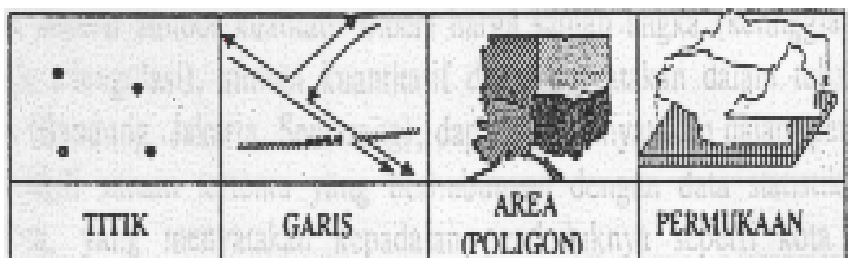
\includegraphics[width=1\textwidth]{figures/dataspasial.JPEG}}
	\caption{data spasial berikut berupa titik, garis, poligon (2-D), permukaan (3-D).}
	\label{dataspasial}
	\end{figure}

Dan arti dari gambar diatas adalah :
Format Titik 						
- Memiliki koordinat tunggal 		
- Tanpa memiliki panjang 			
- Tanpa memiliki luasan

Format Garis
- memiliki koordinat titik awal dan akhir		
- memiliki panjang tanpa luasan

Format Poligon 					
- memiliki koordinat titik awal dan akhir
-memiliki panjang dan luasan 		

Format Permukaan
- memiliki area koordinat vertikal
- memiliki area dengan ketinggian

\item Information
Informasi berasal dari kata pengolahan sejumlah data. Di dalam GIS informasi mempunyai
volume terbesar. Dan setiap object geografi memiliki setting datanya tersendiri karena 
tidak sepenuhnya data yang ada dapat terwakili didalam peta. Maka, semua data harus
diasosiasikan pada objek spasial yang mampu membuat peta menjadi intelligent.

\item System
Pengertian dari suatu sistem merupakan kumpulan elemen-elemen yang saling berintegrasi 
dan berinterdependensi dalam sebuah lingkungan yang dinamis untuk mencapai tujuan tertentu.
\end{enumerate}

\subsection{Definisi GIS (Geography Information and System)}
Dan defenisi dari GIS dapat selalu berubah karena GIS adalah bidang kajian ilmu 
dan teknologi yang masih baru. Beberapa defenisi dari Geographical Information System yaitu:
\begin{enumerate}
\item Definisi GIS menurut(Rhind, 1988):
yaitu : GIS is a computer system for collecting, checking, integrating and analyzing
information related to the surface of the earth.

\item Definisi GIS menurut(Marble \& Peuquet, 1983) and (Parker,
1988; Ozemoy et al., 1981; Burrough, 1986):
yaitu : GIS deals with space-time data and often but not necessarily, employs computer
hardware and software.

\item Difinisi GIS menurut (Purwadhi, 1994):
- SIG adalah suatu sistem yang mampu mengorganisir perangkat keras (hardware),
perangkat lunak (software), dan data, serta dapat mendaya dan digunakan sistem
penyimpanan, pengolahan, maupun analisis data yang dilakukan secara simultan, sehingga dapat
diperoleh seluruh informasi yang berkaitan secara langsung dengan aspek keruangan.
- SIG adalah manajemen data spasial dan data non-spasial yang berbasis komputer
dengan menggunakan tiga karakteristik dasar, yaitu: 
(i) memiliki fenomena yang aktual (variabel data non-lokasi) dan berhubungan 
dengan topik permasalahan di lokasi bersangkutan; 
(ii) merupakan suatu kejadian di suatu lokasi tertentu; 
(iii) memiliki dimensi waktu. Alasan GIS dibutuhkan adalah karena untuk data spasial 
penanganannya sangat sulit karena peta dan data statistik cepat mengalami kadaluarsa 
sehingga tidak ada pelayanan penyediaan data dan informasi yang diberikan menjadi tidak akurat.
\end{enumerate} 

Berikut merupakan keistimewaan analisa dengan Geographical Information System (GIS) yaitu:
\begin{enumerate}
\item Analisa Proximity
Analisa Proximity adalah geografi yang berbasis pada jarak antar layer.
Didalam analisis proximity GIS menggunakan proses yang disebut dengan buffering
yaitu membangun lapisan pendukung sekitar layer dalam jarak tertentu agar dapat menentukan
dekatnya hugungan antara sifat bagian yang ada.
\item Analisa Overlay
Analisa Overlay adalah proses integrasi data dari lapisan-lapisan layer yang berbeda (overlay).
Yang secara analisa membutuhkan lebih dari satu layer yang akan ditumpang susun secara
fisik agar dapat dianalisa secara visual.
\end{enumerate}

Maka artikel :
	Dalam sebuah artikel dari husein yang menyebutkan bahwa  GIS merupakan pemahaman dari
	Geography, Information dan System \cite{husein2006konsep}.

\section{Geographic Information System (GIS): Introduction to the computer perspective}
Sistem Informasi Geografi (GIS) diartikan sebagai sistem untuk menyimpan, memeriksa, 
mengintegrasi, memanipulasi, menganalisis dan memaparkan data yang berkaitan dengan semua 
ruang yang berhubungan dengan keadaan bumi.
Maka artikel :
	Dalam sebuah artikel dari prahasta yang menyebutkan bahwa  GIS merupakan menyimpan, memeriksa, mengintegrasi, memanipulasi, menganalisis dan memaparkan data yang berkaitan dengan semua ruang yang berhubungan dengan keadaan bumi., Information dan System \cite{prahasta2009sistem}.

\subsection{Pengenalan GIS atau Geography Information System}
1. GIS atau dikenal dengan Sistem Informasi Geografi ditunjukan sebagai sistem yang mampu menyimpan, memeriksa, mengintegrasikan, memanipulasi, menganalisis dan memaparkan data-data yang terkait dengan spasial yang merunjuk terhadap bagian bumi. (Jabatan Alam Sekitar, 1987).

2. GIS merupakan satu set lat untuk mengumpulkan, menyimpan, mendapatkan, mengubah dan memaparkan data ruang dari keadaan  bumi yang sebenarnya untuk keperluan tertentu (Burrough, 1986).

3. GIS adalah setiap set manual atau prosedur komputer yang digunakan untuk menyimpan dan memanipulasi data geografis yang tersedia (Arronoff, 1989).

4. GIS merangkum keadaan bumi dengan peranti atau perangkat tertentu yang digunakan untuk peta input atau peta produk, bersama-sama dengan dengan sistem komunikasi yang diperlukan untuk dijadikan sebagai penghubung berbagai unsur. (Star \& Ester, 1990).

5. GIS adalah suatu sistem untuk membantu dalam membangunkan model tertentu yang mustahil untuk dijadikan sintesi data yang banyak. (Martin, 1996).

\subsection{Komponen GIS atau Geography Information System}
Komponen GIS sendiri dibagikan menjadi 3 komponen, yaitu :
Sistem Komputer (perkakas dan sistem operasi), Software GIS
(ArcGIS), database GIS, methode GIS (Prosedur analisis), People (Orang-orang yang menggunakan GIS/User).
Pada gambar \ref{komponenGIS} dijelaskan bahwa kompnen GIS sebagai berikut.

\begin{figure}[ht]
	\centerline{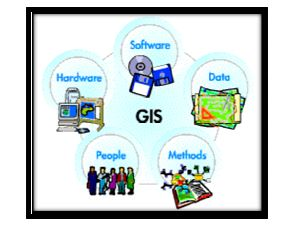
\includegraphics[width=1\textwidth]{figures/komponenGIS.JPG}}
	\caption{komponen GIS.}
	\label{komponenGIS}
	\end{figure}

\subsubsection{Komponen GIS atau Geography Information System}
sesuai dengan gambar diatas komponen GIS dibagi menjadi 3 bagian, yaitu :
1. Sistem Komputer (perkakas dan sistem operasi), merupakan hardware dari sebuah sistem GIS. Perkakas terdiri dari monitor, unit sistem atau CPU, keyboard dan mouse (Heywood et al., 2002). Teknologi komputer harus memiliki kemampuan kuasa
yang tinggi untuk menjalankan perisian GIS.

2. Software GIS , merupakan ArcGIS untuk tujuan perancangan, pengurusan ataupun pemodelan pada kebutuhan tertentu.

3. Database GIS , merupakan tempat yang melibatkan data GIS baik data spatial dan pengurusan datanya. memori untuk menyimpan jumlah data yang besar dan mempunyai kualitas yang baik dengan resolusi tinggi pada skrin grafik warna (untuk membantu dalam menentukan maklumat yang dihasilkan atau diberikan melalui penggunaan warna yang berbeda).

4. Methode GIS , merupakan prosedur dari analisis sistem GIS. yang melibatkan proses input, proses menyimpan, proses mengurus, proses menukar, proses menganalisis, dan proses output yang hanya melibatkan perisian GIS untuk mengatur sistem dan data-data tersebut (Heywood et al., 2002 )

5. People , merupakan orang-orang yang menggunakan sistem GIS. atau orang yang mengendaliakn proses input-output sistem GIS. 

\subsection{Kaedah GIS atau Geography Information System}
Berdasarkan pemahaman diatas, kaedah GIS juga merupakan salah satu komponen penting untuk mengatur sistem GIS sesuai dengan penjelasan sebelumnya. Kaedah-kaedah ini terdiri dari input
data spatial, pengurusan data atribut, paparan data, penerokaan data, analisis dan pemodelan data GIS;
yang dijelaskan oleh gambar sebagai berikut:
Pada gambar \ref{kaedahGIS} dijelaskan bahwa kaedah GIS sebagai berikut.
\begin{figure}[ht]
	\centerline{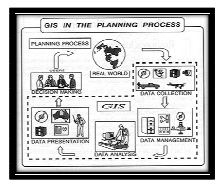
\includegraphics[width=1\textwidth]{figures/kaedahGIS.JPG}}
	\caption{kaedah GIS.}
	\label{kaedahGIS}
	\end{figure}

\subsubsection{Kaedah GIS atau Geography Information System}
1. Input data spatial
Merupakan langkah awal agar terciptanya data baru, dengan cara menginputkan data dan sistem GIS akan menyuntingnya dalam bentuk transformasi geometri yang nantinya akan menghasilkannya kedalam bentuk hard copy. (Chang, 2008) 
(Heywood et al., 2002).

2. Pengurusan data artibut
Merupakan langkah selanjutnya agar sumber peta dapat dipindahkan kepada peta digital yang dapat dibaca oleh GIS.
(Chang, 2008) (Worboy \& Duckham, 2003) (Heywood et al., 2002)

3. Pengumpulan data
Merupakan aktivitas untuk proses melakukan eksplorasi lebih jauh dalam meneliti ciri kesamaa dalam suatu graf peta yang berbeda. (Worboy \& Duckham, 2003).

4. Analisis data
Merupakan cara untuk memaparkan dan memanipulasi data yang didapat. Dengan menggunakan 2 jenis format, yaitu :
- data vektor : melibatkan beberapa kaedah seperti penimbalan / buffering, penindihan/overlay, pengukuran jarak, statik ruang, dan manipulasi peta.
- data raster : menaganalisis pengumpulan data tempatan, kaedah kejiranan, kaedah berzon, dan kaedah operasi global.
(Chang, 2008) (Worboy \& Duckham, 2003) (Heywood et al., 2002)

5. Paparan data dan output data
Dasarnya disediakan untuk tujuan pemaparan hasil dari analisis data yang fungsinya ditujukan untuk pengguna.

6. Aplikasi GIS
Digunakan untuk keperluan tertentu dan bersifat umum bagi masyarakat tergantung keperluan penggunanya. 
(Heywood et al., 2002).

Pada gambar \ref{aplikasiGIS} dijelaskan bahwa aplikasi GIS sesuai keperluan penggunan sebagai berikut.
\begin{figure}[ht]
	\centerline{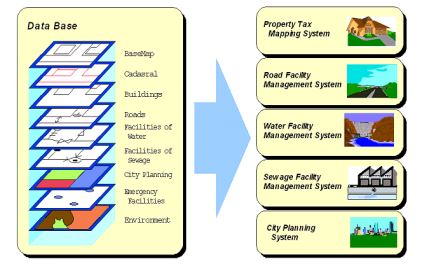
\includegraphics[width=1\textwidth]{figures/aplikasiGIS.JPG}}
	\caption{aplikasi GIS.}
	\label{aplikasiGIS}
	\end{figure}
Maka artikel :
	Dalam sebuah artikel dari hua yang menyebutkan bahwa  GIS memiliki kaedah dan komponen, Information dan System \cite{hua2017sistem}.

\subsection{Kesimpulan GIS atau Geography Information System}
Kesimpulannya, GIS merupakan alat yang penting dalam perspektif komputer pada masa kini dikarenakan GIS
mempunyai kemampuan aplikasi dalam berbagai bidang, misalnya dalam proses perancangan bandar dan kartografi,
penilaian kesan alam sekitar dan pengurusan sumber asli. GIS juga memainkan peranan dalam perspektif perniagaan,
dimana alat ini sangat bermanfaat dalam pengiklanan dan pemasaran, jualan, dan logistik 
mampu digunakan untuk mencari dan meningkatkan perniagaan seperti tapak perniagaan yang strategik. Sebagai umum, pengguna GIS dapat dilibatkan dengan agensi-agensi penguatkuasaan undang-undang, strategi
perancangan, perhutanan, industri, pemberdayaan alam, perencanaan kota, profesional
telekomunikasi, kesehatan, pengangkutan, geografi, dan pembangunan pemasaran. 
Penjelasan ini menyediakan platform untuk memahami lebih lanjut tentang komponen, kaedah, dan aplikasi GIS, 
untuk mempelajari tentang alat GIS.
\subsection{Saran GIS atau Geography Information System}
GIS dapat diaplikasikan di dalam kehidupan sehari-hari untuk memenuhi kebutuhan dan dapat membantu kebutuhan setiap masyarakat menjadi lebih baik dan lebih bermanfaat. Karena dengan memanfaatkan kemajuan teknologi maka teknologi yang digunakan akan ikut turut serta terus perkembang untuk menyesuaikan pemenuhan kebutuhan setiap pengguna yaitu masyarakat. Demikian kesimpulan dan saran yang dapat disampaikan kurang lebihnya mohon maaf dan terimakasih.

\subsection{SIG mempresentasikan real world dengan data spasial yang terbagi atas 2 model data, yaitu:}
1. Vektor, Bumi dalam data vector direpresentasikan sebagai mozaik yang terdiri atas garis, polygon, titik,
dan noders.
Model data vector merupakan model data yang paling banyak digunakan, model ini berbasiskan
pada titik dengan koordinat (x,y) untuk membangun objek spasialnya. Objek yang dibangun
dibagi menjadi tiga bagian, yaitu: titik, garis, dan area (polygon).
Keuntungan dari data vector, yaitu: ketepatan dalam merepresentasikan fitur titik, batasan dan
garis lurus.
2. Raster, Data raster adalah data yang dihasilkan dari sistem pengindraan yang jauh. Pada data raster,
objek geografis direpresentasikan sebagai struktur sel grid yang disebut pixel. Resolusi pada data
raster tergantung pada ukuran pixel-nya.
Maka, resolusi pixel menggambarkan ukuran sebenarnya dari permukaan bumi yang diwakili
oleh setiap pixel pada citra. Semakin tinggi resolusinya, semakin kecil permukaan bumi yang
direpresentasikan oleh suatu sel. Data raster cocok untuk merepresentasikan batas-batas yang
berubah secara gradual, seperti jenis tanah, vegetasi, suhu tanah, dan kelembaban tanah.


\chapter[Sejarah Kutub Utara]
{Pengantar\\ Kutub Utara}
%Kelompok 3
%Kutub Utara
%
%Andi Syahjaratu Daur - 1154092
%Aditya Pratama Dharma - 1154043
%Bendra Wardhana - 1154015
%Dini Islamiani - 1154039
%Nur Rahmawati - 1154124	
%Pembahasan Dan Isi 

\section{Deskripsi Kutub Utara}	

		Dalam artikel Arctic Monitoring and Assessment Programme {AMAP}  ada beberapa masalah yang ada didalam 
	kutub utara, yang paling menonjol adalah masalah polusi dan lingkungan.
		
		Kutub Utara sedang mengalami beberapa hal yang paling cepat dan perubahan iklim berat di bumi. Selama 100 tahun,perubahan
	iklim diharapkan untuk mempercepat, memberikan kontribusi untuk fisik utama, ekologi, sosial, dan perubahan ekonomi, banyak yang 
	telah dimulai. Perubahan iklim kutub utara juga akan mempengaruhi seluruh dunia melalui peningkatan pemanasan global dan meningkatnya permukaan laut. 
	Dampak dari Kutub Utara merupakan dataran tinggi penghangat sintesis bahasa dari temuan-temuan kunci Kutub Utara Dampak Perubahan Iklim {ACIA}, dirancang 
	untuk dapat diakses untuk para pembuat kebijakan dan publik yang lebih luas. Dalam ACIA adalah secara komprehensif diteliti, benar-benar direferensikan,
	dan evaluasi secara independen dari perubahan iklim kutub utara. Ia telah terlibat sebuah upaya internasional oleh ratusan ilmuwan.
	Dalam artikel Impacts of a Warming Arctic - Arctic Climate Impact Assessment ini menyediakan informasi penting kepada masyarakat dan contemplates-respons 
	untuk salah satu tantangan terbesar pada zaman kita.
	
		Northeast Rusia, dan sungai Mackenzie {130 W. panjang.}, Amerika Barat Laut, dan antara Laut Arctic di utara dan selatan Alaska dan
	Kuriles tengah di selatan. Wilayah ini disajikan sebagai suatu negeri-jembatan antara Eurasia dan Amerika Utara di seluruh Tertiary sehingga kira-kira 5 Ma
	ketika ia diputuskan oleh pembentukan Bering Strait {Marincovich \& Gladenkov 1999, 2001}. Selama Kuartenari, tanah-pembaharuan bridge selama glaciations 
	utama bila tingkat laut jatuh oleh 100-135 m {Hopkins 1973; Clark \& Mencampur 2002}.Northeast Rusia dan Amerika Barat Laut {Alaska dan Yukon} tetap bebas es 
	selama Kuartenari glaciations dan melayani sebagai refugium utara besar-besaran untuk kutub utara dan boreal biota.Wilayah ini Beringia Hultén dipanggil dan
	didefinisikan sebagai kawasan antara Sungai Lena {125 E. panjang.}, Northeast Rusia, dan sungai Mackenzie{130 W. panjang.}, 
	Amerika Barat Laut, dan antara Laut Arctic di utara dan selatan Alaska dan Kuriles tengah di selatan.Wilayah ini disajikan sebagai suatu negeri-jembatan antara 
	Eurasia dan Amerika Utara di seluruh Tertiary sehingga kira-kira 5 Ma ketika ia diputuskan oleh pembentukan Bering Strait {Marincovich \& Gladenkov 1999, 2001}. 
	Selama Kuartenari, tanah-pembaharuan bridge selama glaciations utama bila tingkat laut jatuh oleh 100-135 m {Hopkins 1973; Clark \& Mencampur 2002}.
	
\subsection{Kutub Utara Tahun ini}

		Dalam Kuartenari {kira-kira 2 Ma hingga sekarang} distribusi dan komposisi kutub utara flora ini sangat dipengaruhi oleh terlebih dahulu dan mundur dari 
	lapisan-lapisan ais. Secara tradisional, ia berpikir bahwa selama periode seretnya proses semua wilayah utara tertutup oleh es ke sejauh serupa dan bahwa
	binatang dan tumbuhan kutub utara bermigrasi ke selatan memajukan lembaran-es untuk bertahan hidup di selatan refugia {Darwin tahun 1859; Hooker tahun 1862}.
	Namun, keyakinan ini menghadapi tantangan dalam 1937 oleh bahasa Swedia botanis, Eric Hultén, dalam bukunya garis besar tentang sejarah Kutub Utara dan 
	Boreal Biota selama periode divisi kuartenari. Hultén menarik pada bukti geologi dan tubuh yang luas dari bukti phytogeographical sendiri, untuk mengusulkan
	bahwa kebanyakan dari Northeast Rusia dan Amerika Barat Laut {Alaska dan Yukon} tetap bebas es selama Kuartenari glaciations dan melayani sebagai refugium 
	utara besar-besaran untuk kutub utara dan boreal biota {Gbr. 1}. Wilayah ini Beringia Hultén dipanggil dan didefinisikan sebagai kawasan antara Sungai Lena 
	{125 E. panjang.}
		Kutub Utara tahun ini terdiri dari kira-kira 1.500 spesies flora dan yang relatif baru asal usul {Murray 1995}. Perguruan Tinggi di sebagian besar {65-2 Ma}, 
	hutan tumbuh di ketika latitud tinggi di Kutub Utara {Murray 1995; McIver \& Basinger 1999} dan tundra tidak muncul hingga akhir Pliocene {Salasila Matius \& Ovenden 1990}.
	Pada awalnya tundra ini disebarluaskan discontinuously, tetapi sebuah sabuk circumarctic hadir dengan 3 Ma {Salasila Matius 1979}. 
	Sedikit yang diketahui tentang asal usul tumbuhan kutub utara, walaupun ianya diandaikan bahawa banyak tanaman tersebut berasal dari saham nenek moyang yang terjadi 
	di gunung-gunung yang tinggi, di sebelah selatan di Asia dan Amerika Utara {Hultén 1937; Tolmachev 1960; Weber 1965; Hedberg 1992; Murray 1995}. Gunung ini membentuk 
	bagian dari berkisar antara terhubung ke Kutub Utara, di sepanjang tanaman yang dapat bermigrasi ke arah utara, seperti suhu global turun secara signifikan dari 
	pertengahan Miocene dan seterusnya {Lear et al. 2000; Zachos et al. 2001}. Selain itu, beberapa tanaman kutub utara mungkin berasal dari shrubby dan elemen-elemen 
	herbaceous hutan kutub utara yang menduduki Tersier membuka, dan riparian {40-2}-habis sama sekali habitat dataran tinggi di Kutub Utara selama akhir 
	Tertiary {Murray 1995}.
	
\begin{figure}[ht]
\centerline{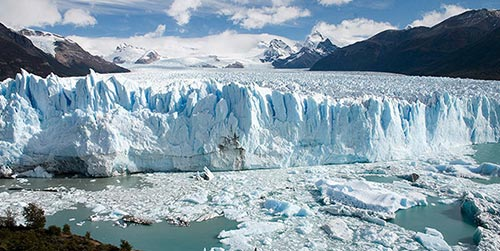
\includegraphics[width=1\textwidth]{figures/arctic.jpg}}
\caption{Menjeleskan tentang kutub utara.}	
\label{Kutub_Utara}
\end{figure}
	
\subsection{Pemanasan di kutub utara}
		Metana di dalam atmosfir kutub utara telah meningkat dengan tajam sebanyak 33% dalam kurun 5 tahun tanah es yang mencair di siberia telah melepaskan 5x 
	jumlah metana dari yang sebelum nya di prediksi permafrost dangkal bawah laut pada kutub utara juga menunjukan ketidak stabilan dan melepaskan jumlah metana
	yang banyak padang rumput pada kutub utara pada saat ini sudah mengeluarkan lebih banyak metana dan nitrogen oksida dari perkiraan yang sebelumnya ilmuan 
	telah memberi nama pencairan kutub utara dengan nama bom waktu yang berdetak, Kutub utara memanas dua kali lebih cepat di bandingkan tempat lain yang berada
	di bumi tanpa es yang melindungi untuk memantulkan sinar matahari , di dunia terdapat dua lapisan es besar yaitu greenland dan kutub selatan Kutub utara merupakan
	negara yang mustahil untuk di tempati makhluk hidup namun juga terdapat beberapa spesies fauna yang dapat hidup disana salah satu nya adalah beruang kutub
	meski memiliki tubuh yang besar beruang kutub mampu berenang selama berhari-hari di perairan terbuka dan sanggup menjangkau jarak ratusan kilometer .

\begin{figure}[ht]
\centerline{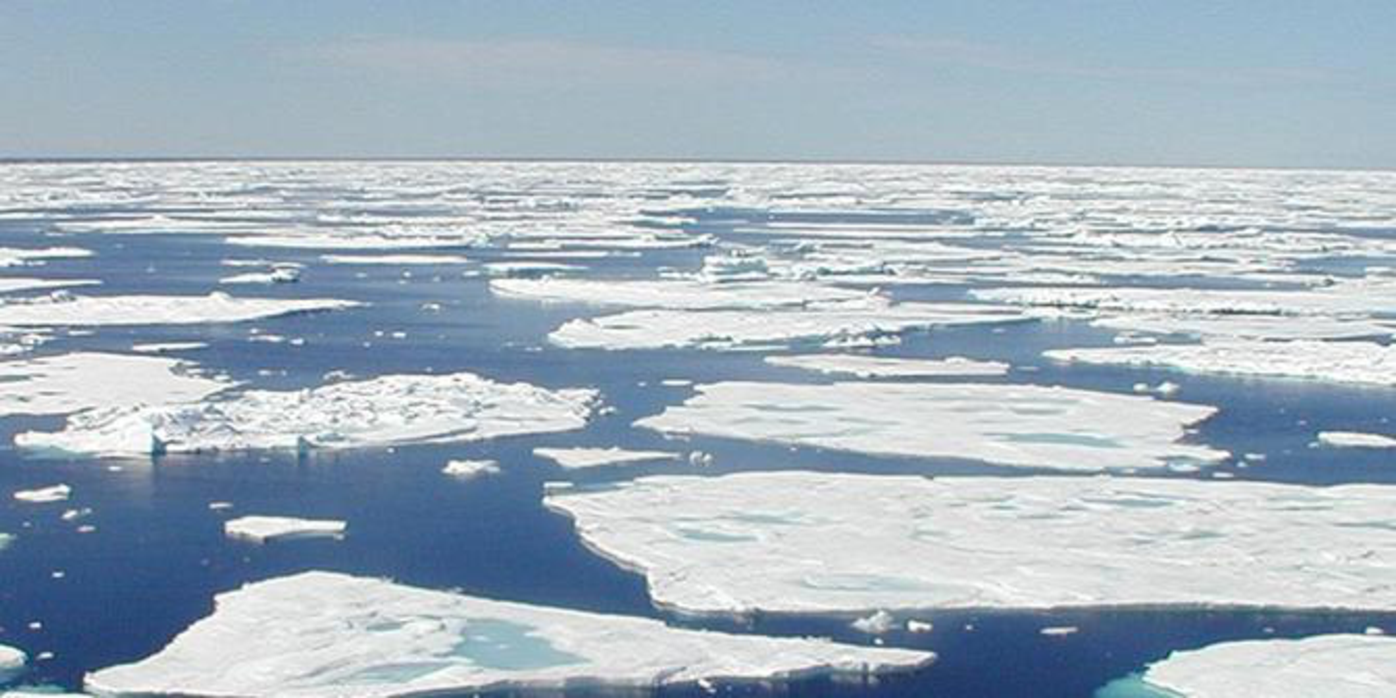
\includegraphics[width=0.5\textwidth]{figures/arctic1.pdf}}
\caption{Menjeleskan tentang pemanasan kutub utara.}	
\label{Pemanasan_Kutub_Utara}
\end{figure}

Pada gambar \ref{Pemanasan_Kutub_Utara} menjelaskan tentang pemanasan di kutub utara.

\subsection	{Kutub Utara}	ari 2 meter lebih pada 50 tahun 
	mendatang. Upaya untuk mengatasi tantangan perubahan iklimdan kenaikan permukaan laut tersebut, kota Rotterdam telah membangun beberapa struktur terapung 
	berdesain unik dan menarik, Dan Menurut nanang rianto dampak pencairan es di Kutub Utara dan Selatan akibat pemanasan global,dan gejala penurunan elevasi
	tanah (land subsidence).
	
		Kutub utara diramalkan akan punah karena habitatnya yang mengecil.bobot hewan itu mengalami penyusutan signifikan dalam dekade
	akhir ini.Makanan beruang adalah ikan,Mereka mencarinya dengan membuat lubang di lapisan es sehingga ketika ada ikan lewat langsung disambarnya.sekarang 
	jangankan membuat lubang mencari tempat berpijak saja susah karena banyaknya es yang mencair sehingga beruang harus sering melompat berpindah balok es.
	Tak jarang pun ikan susah ditangkap.beruang kutub harus berenang bermil-mil demi mendapatkan tempat baru, dan ini berisiko besar karena domain beruang
	kutub bukanlah dilaut.
	
	
\subsubsection {Kutub Utara}
		Kutub utara magnet bumi untuk diinterpretasi. Hasil interpretasi kualitatif menunjukkan bahwa pada peta anomali regional terdapat anomali dipole magnetik
	yang membentang dari arah barat daya ke timur laut Semenanjung Muria, Peta anomali lokal menunjukkan dua buah anomali dipole magnetik yang membentang dari 
	arah barat laut ke tenggara di sebelah utara dan barat kompleks Gunungapi Muria, dan satu pasang dipole magnetik di tenggara Gunungapi Muria Hasil 
	interpretasi kuantitatif yang dilakukan dengan menggunakan software Mag2DC for Windows. Pada anomali regional dan anomali lokal yang direduksi ke kutub 
	terdapat sebuah sesar di sebelah tenggara gunungapi Muria, tepatnya pada daerah Maar Gunung Rowo. Struktur geologi bawah permukaan daerah Gunungapi Muria 
	dan Maar Gunung Rowo berdasarkan harga suseptibilitas batuan dikontrol oleh batuan vulkanik yang terdiri dari andesit dari satuan batuan Lava Muria, tufa 
	dari satuan batuan Tuf Muria, batupasir tufaan dari formasi Patiayam, batugamping dari formasi Bulu, dan batulempung dari formasi Ngrayong. Pada kedalaman
	7-15 km di bawah permukaan terdapat batuan vulkanik dan vulkanik klastik yang merupakan batuan dasar penyusun Semenanjung Muria.
	
\subsubsection{kutub utara magnet diinterpretasi}
		Kutub utara magnet bumi untuk diinterpretasi. Hasil interpretasi kualitatif menunjukkan bahwa pada peta anomali regional terdapat anomali dipole 
	magnetik yang membentang dari arah barat daya ke timur laut Semenanjung Muria, Peta anomali lokal menunjukkan dua buah anomali dipole magnetik yang 
	membentang dari arah barat laut ke tenggara di sebelah utara dan barat kompleks Gunungapi Muria, dan satu pasang dipole magnetik di tenggara Gunungapi
	Muria Hasil interpretasi kuantitatif yang dilakukan dengan menggunakan software Mag2DC for Windows. Pada anomali regional dan anomali lokal yang direduksi
	ke kutub terdapat sebuah sesar di sebelah tenggara gunungapi Muria, tepatnya pada daerah Maar Gunung Rowo. Struktur geologi bawah permukaan daerah 
	Gunungapi Muria dan Maar Gunung Rowo berdasarkan harga suseptibilitas batuan dikontrol oleh batuan vulkanik yang terdiri dari andesit dari 
	satuan batuan Lava Muria, tufa dari satuan batuan Tuf Muria, batupasir tufaan dari formasi Patiayam, batugamping dari formasi Bulu, dan 
	batulempung dari formasi Ngrayong. Pada kedalaman 7-15 km di bawah permukaan terdapat batuan vulkanik dan vulkanik klastik yang merupakan 
	batuan dasar penyusun Semenanjung Muria.
	
\subsubsection {kutub utara terendam}
		Menurut artikel Fatmasari Savitri, Eddy Prianto, Erni Setyowati i kutub utara dan selatan bumi akan terendam lebih dari 2 meter lebih pada 50 
	tahun mendatang. Upaya untuk mengatasi tantangan perubahan iklim dan kenaikan permukaan laut tersebut, kota Rotterdam telah membangun beberapa 
	struktur terapung berdesain unik dan menarik. 
	
\subsubsection {kepunahan habitat kutub utara}
		Kutub utara diramalkan akan punah karena habitatnya yang mengecil.bobot hewan itu mengalami penyusutan signifikan dalam dekade akhir ini.
	Makanan beruang adalah ikan,Mereka mencarinya dengan membuat lubang di lapisan es sehingga ketika ada ikan lewat langsung disambarnya.sekarang 
	jangankan membuat lubang mencari tempat berpijak saja susah karena banyaknya es yang mencair sehingga beruang harus sering melompat berpindah 
	balok es.Tak jarang pun ikan susah ditangkap.beruang kutub harus berenang bermil-mil demi mendapatkan tempat baru, dan ini berisiko besar karena 
	domain beruang kutub bukanlah dilaut.
	
		




\chapter[Tentang Kutub Selatan]
{Pengantar\\ Antartika}
%Kelompok 2
%DONI SAPUTRA(1154030)
%CAHYA KURNIAWAN(1154038)
%IKA SYAM SETIAWATI(1154054)
%SILVY DHARMA FEBRYANA(1154112)
%WIDI DAMAYANTI(1154062)
%ANTARTIKA


																		
Pembahasan Dan Isi 

\begin{figure}{ht}
\centerline{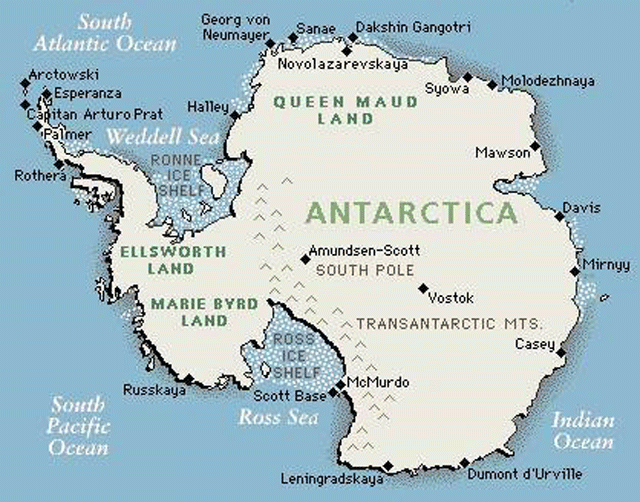
\includegraphics[width=1\textwidth]{figures/antartic.PNG}}
\caption{Menjelaskan tentang benua antartika.}
\label{Antartika}
\end{figure}

\section{Deskripsi Antartika}



		Benua antartika adalah suatu wilayah laut perifer yang merupakan sumber informasi utama pada cryosphere cenozoik dan peristiwa 
	kejadian yang mengarah pada perkembangan kurang lebih 36 juta tahun yang lalu. Dilihat dari berbagai data sekarang sudah terlihat bahwasanya 
	garis lintang selatan sudah mengalami perubahan dinamika ekspansi pada lapisan lapisan es nya dan pembusukan melewati akhir Palaeogene dan Neogene. 
	Pada ejarah perubahan iklim disertai dan sangat di pengaruhi oleh lithosphere vertical dan horizontal yang sangat signifikan. Peristiwa perubahan, 
	termasuk evolusi seaways internal utama dan pegunungan. \ref{Antartika}
		
		Meskipun penyidikan yang dilakukan di tahun pertama pada abad ini antartika kenozoikum penelitian ini adalah bagian dari beberapa kegiatan yang 
	relative memanjang di sedikit lebih dari 3 dekade di bagian lain dari bumi, kenozoikum rentan terhadap satu penyeledikan, dan dalam sejumlah perkara, 
	hampir 2 abad. Situasi ini sebagian besar dari bagian antartica. Yang sulit adalah penelitian lingkungan, keterbatasan peanfaatan teknologi canggih, 
	dan realisasi tertunda. Sebagai pentingnya selat lintang selatan yang tinggi untuk isu-isu global, tektonik evolusi seperti  palaeogeography, 
	palaeo-oceanography, biogeography, evolusi, dan palaeoclimate biotik. Meskipun komprehensif tinjauan kenozoikum sekarang sudah membuat penampilan yang baru 
	tetapi 25 tahun lalu konozoikum geologi dari antartika hanya mampu melayani beberapa saja.
	
		Terdapat perbedaan yang menarik dalam cara di mana dan kenozoikum pre-cenozoic studi yang telah dikembangkan di antartika.
	Penelitian dan pendalaman palaeozoic di mesozoikum dan gondwana  geologi yang berfungsi sebagai contoh yang baik .Pada akhir 1950s , 
	ahli geologi banyak dari negara negara berkumpul di antartika dengan cukup detail stratigraphic palaeontological dan informasi dan banyak pengalaman 
	dari banyak tahun penelitian di satu fragmen mantan supercontinent gondwana.Dalam hal kotor, para palaeozoic-mesozoic stratigraphy antartika 
	cermin melaporkan bahwa dari afrika selatan , india , australia , dan amerika selatan .Antartika palaeozoic-mesozoic disebut ilmu pengetahuan untuk 
	memberikan untuk mengukur daerah , stratigraphy , koleksi fosil , analisis dan batuan beku sedimen batu dan daerah analisis .Kebanyakan gondwanas  
	para ilmuwan itu , lalu , pengujian dan memperluas pengetahuan dasar yang itu , dalam banyak hal , dikembangkan di beberapa benua. 
	Fosil yang dikumpulkan di Antartika selama 30 tahun telah didokumentasikan dengan baik di wilayah-wilayah lain Gondwana dan penemuan mereka di Antartika 
	telah sering agak tepat memperkirakan. 
	
		Misalnya, dalam sebuah pra-Geofisik Internasional kaji ulang tahun, Fairbridge geologi Antartik (1952, mukasurat 88) dicatatkan, 
	"Maukah membingungkan dari semua adalah ketiadaan bukti seretnya proses di gunung batu zaman Permian, yang merupakan kali mengalami Glaciation 
	kuat dalam semua bagian lain di Selatan Hemi-; mengapa sphere Antartika, dari segala tempat akan dikecualikan.' Dalam satu dekade laporan-laporan 
	sebagai-ke-kemudian hilang tillites dibuat dari Rambu Supergroup dari Trans- Gunung dan lain-lain tempat Antartika. Elemen penting dalam kemajuan yang 
	dibuat oleh Palaeozoic cepat dan para peneliti Mesozoikum adalah mendukung pro- vided oleh IUGS Sub-Commission untuk Gondwana Stratigraphy serta 
	palaeontologi. Para peneliti Cenozoic Antartik tidak memiliki dukungan dari sebuah organisasi payung, walaupun IUGS Kuartenari Internasional Association 
	mungkin telah memainkan peran lebih aktif, terutama di daerah seretnya proses dan proses interglacial Antartika. Studi Cenozoic Antartik kekurangan, 
	antara lain, sebuah elemen prediktif, dan banyak kemajuan yang telah serendipitous, selalu mengherankan, dan sering kontroversial. 
	Antartika, geografis belaka pencerahan telah, untuk tiga dekade terakhir, dijamin tingkat geografis, dan isolasi intelektual untuk pekerja Cenozoic 
	dari banyak negara. Sementara ada sebuah koleksi tingkat kuat dan dokumentasi, hanya ada sedikit koordinasi dan jangka panjang perencanaan di antara 
	berbagai perusahaan nasional. Dalam jumlah relatif kecil melimpahnya sinar Cenozoic di Antartika sekarang dengan cukup lancar didokumentasikan dan 
	sedikit yang dapat diperoleh didaur ulang usaha sebelumnya hanya untuk penguatan marjinal. Kita harus berkonsentrasi pada cara-cara untuk kausingkapkan 
	98% dari geologi Cenozoic kita masih belum menemukan! Lebih penting lagi, kita harus melihat 'austral' Cenozoic di lebih ketentuan global.
	\cite{peter1990Antartica}.
	

\subsection{Antartika dan Cenozoic cryosphere}

		Jika seseorang untuk satu dari satu fenomena geologis yang disajikan untuk menyorot pentingnya Cenozoic Antartika ia harus realisasi yang tinggi 
	selatan latitude Cenozoic perubahan iklim goyangan) yang dicetuskan dampak yang signifikan yang jauh melampaui batas benua untuk sekurang-kurangnya 
	dua pertiga dari waktu Cenozoic. Setelah Ia mengatakan semuanya itu, satu juga harus mengamati bahwa penelitian Cenozoic Antartika dan global 
	masyarakat telah, hingga sangat baru-baru ini, bekerja secara mandiri dan terlepas dari satu sama lain dan telah ada unawareness umum oleh mantan 
	kelompok yang berkembang pesat Cenozoic Antartik alas data dan kompleksitas seretnya proses-proses deglacial. Untuk banyak palaeo-ahli lautan, 
	ia telah atribut yang cukup untuk 'dingin' tren data proxy mereka untuk 'cryogenic' kejadian ke selatan, barangkali glaciation di Antartika. 
	Dalam beberapa tahun terakhir telah melihat sebuah sambutan pindah ke arah yang lebih besar di tingkat interaksi antara kedua masyarakat. 
	Namun, masih lebih banyak dan integratif dasar research untuk dapat dicapai dalam dan antara wilayah dan alas data kelautan.
	
	
\subsection{Peran dari laut dalam Proyek pengeboran dan laut Program Pengeboran}
		
		memiliki banyak untuk mengubah studi Cenozoic global dari sebagian besar aktivitas berbasis tanah untuk satu spanning hampir di seluruh bumi. 
	High latitude pengeboran usaha-usaha kaki 28 (selatan-timur Laut Ocean-Ross OceanSouthem India di tahun 1973), 35 (selatan-timur Samudera Pasifik di 1974), 
	113 (Laut Weddell- Samudera Atlantik Selatan pada tahun 1987), 114 (subantarctic Samudera Atlantik Selatan pada tahun 1987, 
	119 (Prydz Bay-Southern Samudera India pada tahun 1988) dan 120 (dataran tinggi Kerguelen-selatan-timur Samudera India pada tahun 1988) telah dilakukan 
	banyak untuk membawa bersama-geologi Cenozoic dari Antartika dan subantarctic yang tepat dan ketika latitud temperate (Gbr. 1). 
	Sementara banyak rincian empat kaki Antartik masih menunggu,-peri- kapal penyelidikan berbasis Antartika, bersama-sama dengan penelitian pada benua itu 
	sendiri, telah memperkuat pemahaman kita tentang kedua-dua dahulukala dan sejauh mana Cenozoic glaciation di belahan bumi selatan.
	

\subsection{evolusi Cenozoic Palaeoenvironments di Selatan}

		Pada tahun 1986, Sidang Internasional Perserikatan Ilmiah (ICSU) Komite Ilmiah pada Antarctic Research (mengenai pelipis) didirikan grup dari 
	kalangan dokter spesialis pada evolusi Cenozoic Palaeoenvironments di Selatan ketika latitud tinggi. Perintah kepada kelompok internasional ini 
	disertakan: korelasi dan integrasi terresulal Antartika dan Cenozoic palaeoenvironmentalr ecords laut dengan orang-orang di selatan ketika latitud 
	tinggi, dan pengakuan dan evaluasi gfobal Cenozoic penting, palaeu tektonik mengadakan dan peristiwa palaeoclimatic-disimpulkan dari penelitian 
	geologi Antartika. Dalam tiga tahun terakhir dalam grup bekas luka dari kalangan dokter spesialis telah berpartisipasi dalam beberapa dinner symposia 
	dan telah menyetel tentang mengkaji topik Cenozoic penting di lokakarya khusus. Misalnya, pada akhir 1988 Grup dari kalangan dokter spesialis 
	mensponsori 'Lokakarya Pengeboran Kutub' dalam kerjasama dengan Yayasan Sains Nasional AS; dan pada awal 1989 mengadakan pertemuan pada geochronology 
	Cenozoic Antartika. Pertemuan masa depan dan ini berfokus pada topik-topik yang dianggap penting, terutama dalam memahami peran global 
	geologi Cenozoic Antartik.
	
	
\subsection{Program Geosphere-Biosphere Internasional}

		Dengan penyebaran ICSU 'Geosphere Internasional- Program Biosfir'(IGBP),p olar para peneliti Cenozoic dihadirkan dengan beragam peluang baru. 
	Baru-baru ini bekas luka mengakui peran utama dalam wilayah kutub selatan harus memainkan di masa depan oleh penerbitan 'Peran Antartika dalam 
	Perubahan Global' (ICSU Tekan). Inisiatif IGBP yang prihatin prinsipnya dengan (p. 7), 'interaksi kunci dan perubahan yang signifikan pada waktu 
	timbangan dekade untuk berabad-abad...."; namun, pada mukasurat 23 dinyatakan, 'Antartika berpendapat rekod ekstensif iklim masa lalu dan perubahan lingkungan. 
	Inti es dan core laut dapat menumpahkan lampu baru seperti pada perubahan. Dari permukaan particularpromisea re-ke-core batu.
	
	
\subsection{Wilayah penting dan daerah yang dikenali sejak tahun Geofisik Internasional (1957-1708)}

		Tahap sekarang penyelidikan bermula pada 1957 selama Tahun Geofisik Internasional. Selama penyelidikan selama 30 tahun beberapa wilayah kunci 
	muncul sebagai penting, terutama. Ini adalah: Seymour Island, dengan terkena Cretaceous-Palaeocene penting- Eocene successions, dan remarkablef 
	fossil faunas dan floras: Raja George Island, dengan Eocene-Oligocene penting-Miocene successions lebih rendah dari fossiliferous sedimen glacigene 
	laut dan interbedded dapat ditarikhkan volcanics: dan selatan- Ross Barat Laut (Victoria Tanah Basin dan bokor lainnya) dan berdekatan dengan wilayah 
	Gunung Transantarctic, dengan Oligocene-MiocenePliocene-Pleistocene glacigene penting di diantaranya- cessions (Gbr. 1). 
	Baru-baru ini, Amery graben-Wilkesfpensacola Prydz Bay dan bokor-bokor penyiraman juga telah menjadi wilayah penting untuk Palaeogene dan studi Neogene. 
	Mayoritas Cenozoic Antartik literatur selama tiga dekade terakhir berasal dari lapangan dan penyelidikan laboratorium di wilayah dipisahkan secara luas ini.
	Sementara Cenozoic outcrops di wilayah-wilayah ini berisi floras macrofaunasa yang sangat baik ke-52, dan telah dikaitkan dalam beberapa contoh dengan 
	dapat ditarikhkan bahan gunung berapi, hanya rovide successionsp temporal kesinambungan sporadis. Hiatuses adalah biasa dan banyak-kurang bergandengan usia. 
	Sementara kutub dan extra-palaeo kutub-mengadakan dan peristiwa iklim telah didokumentasikan dalam negeri-basedexposures ini, 
	ia juga jelas bahwa stratigraphicalr ecord tidak memadai untuk spektrum luas Cenozoic studi geologi.
	
	
\subsection{Pengeboran ilmiah (1972-1954)}

		Sejak tahun 1972, serangkaian pengeboran ilmiah ventures telah sangat memperbaiki geografis, dan jangkauan temporal untuk kedua-dua Palaeogene 
	dan Neogene (buah ara 1,2,3). 70 lubang simulasi selesai dalam 18 tahun terakhir jatuh ke dalam dua kategori utama. 3 1 situs-situs menaruhnya di darat 
	atau dari laut dekat pantai-platform es, dengan total penetrasi 3793 m (12 444 kaki), dan 39 kapal laut dalam simulasi berbasis lubang-lubang.
	
	diperhatikan di bawah bahwa latitudepalaeogene tinggi selatan dan rekaman Neogene kompleks interelated frekuensi tinggi mengadakan geologis, 
	peristiwa iklim dan, banyak di antaranya yang hanya dapat diatasi jika sampling adalah pada 25 untuk 50 000 tingkat tahun. Sedikit kemajuan akan dibuat 
	dalam palaeoenviron- dan studi palaeoclimatological mental tanpa peningkatan yang signifikan dalam penggunaan teknologi pengeboran yang paling maju 
	di kedua Antartika dan di wilayah subantarctic.
	

\subsection{Pelat dan interaksi microplate}

		Pelat dan interaksi microplate disintegrasi Gondwana dalam Mesozoic dan Cenozoic, menjadi kecil continental pelat dan microplates, disediakan rumit 
	dan pernah mengubah konfigurasi dari tanah dan wilayah laut di bagian selatan ketika latitud tinggi. Pemisahan Australia dan Antartika dalam Eocene, 
	pemisahan di selatan Amerika Selatan semenanjung dari Antartika dekat batas Oligocene-Miocene,t dia subsequentd pembangunan sirkulasi laut sekitar 
	Antartika, dan efek yang dihasilkan pada perubahan iklim dan biogeography telah didokumentasikan dengan baik dalam literatur (lihat Kennet 1982 untuk 
	ringkasan pandangan dan lengkap dari literatur justu berlawanan). Sementara Cenozoic episode tektonik di pinggiran benua tersebut adalah dengan cukup 
	lancar didokumentasikan, orang-orang dalam wilayah pedalaman tidak. Setelah kedua adalah dimengerti dengan baik kita akan lebih mampu untuk menilai 
	pewaktuan dan perutean jalur sirkulasi laut ke dan di Antartika (Gbr. 4). Tidak jelas, misalnya, apakah yang dicurigai dan masa kelam erosional tektonik 
	yang disediakan dalam peredaran air-merutekan sekitar dan melalui bagian Antartika di berbagai waktu selama Cenozoic, dan apakah saluran ini disediakan 
	sebuah link efektif antara berbagai sektor Atlantik selatan, Pasifik dan lautan India. Studi masa depan harus menekankan pembatasan, dan interaksi antara, 
	pelat dan microplates, bersama dengan penentuan masa gerakan vertikal dan horizontal.
	
	
	
	
\begin{figure}{ht}
\centerline{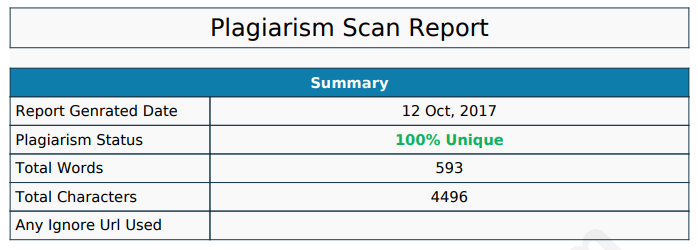
\includegraphics[width=1\textwidth]{figures/plag.PNG}}
\caption{plagiarism}	
\label{plag}
\end{figure}

	
		
	
	
		


%\chapter[Sejarah Penentuan Waktu]
%{Pengantar\\ Sejarah Penentuan Waktu}
%% Kelompok Penentuan Waktu
% Muhammad Nur Ikhsan (1154087)
% Wahyu Maruti Adjie (1154034)
% Ilman Mubarik 	(1154114)
% Emy Safitri		(1154102)
% Andi Ikram Maulana	(1154065)

\section{Sejarah Waktu}
\paragraph{Sejarah Penentuan Waktu diurutkan secara kronlogis dalam sebuah tabel skala waktu geologi 
yang dapat dibagi menjadi beberapa interval sesuai analisis stratigrafi. 
Terdapat 4 garis waktu yang ada, garis waktu yang pertama menunjukkan waktu dari masa-
terbentuknya Bumi sampai waktu sekarang\cite{suryasejarah}. 
Skala waktu kedua menunjukkan eon terbaru dengan skala yang diperluas.} 

\paragraph{Skala waktu kedua, ketiga, dan keempat merupakan sub bagian 
dari skala waktu sebelumnya yang ditunjukkan oleh tanda bintang. 
Alasan lain untuk memperluas skala waktu adalah HOLOSEN (jangka waktu) terakhir 
terlalu kecil untuk dapat ditampilkan dengan jelas
pada skala waktu ketiga disebelah kanan. Gambar \ref{sejarahpenentuan} skala waktu}

\begin{figure}{ht}
\centerline{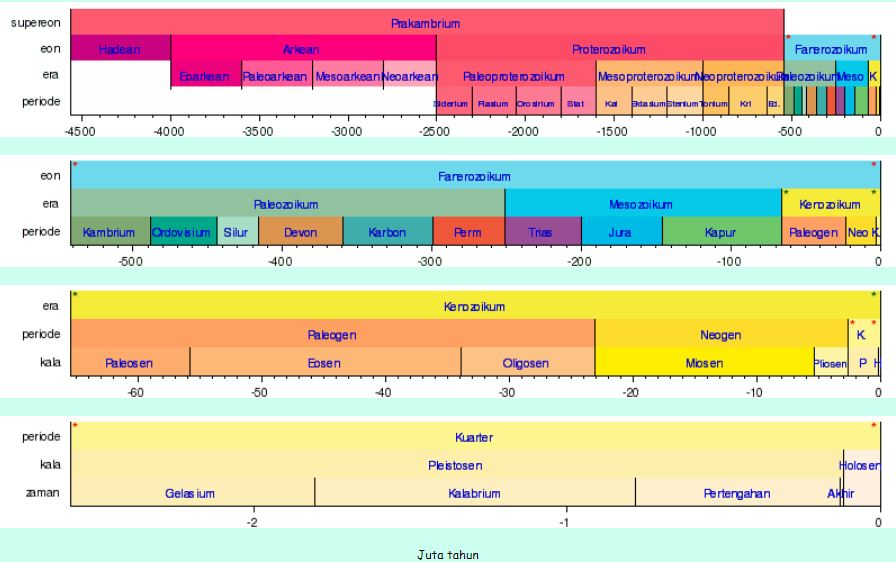
\includegraphics[width=1\textwidth]{figures/sejarahpenentuan.JPG}}
\caption{gambar skala waktu yang ditetapkan.}
\label{sejarahpenentuan}
\end{figure}

\section{Penentuan Waktu}
\paragraph{Pada pembahasan diatas, kita telah membahas tentang sejarah waktu, dan skala waktu. 
Dari penjelasan tersebut, maka dibuatlah suatu pergerakan rotasi bumi. 
Gerakan ini disebut gerakan semu Matahari yang digunakan dalam penentuan waktu (jam).}

\subsection{Hari Matahari}
 \paragraph{Menurut artikel dari rachman planet mengemukakan bahwa satu hari matahari ditentukan
 oleh selang waktu antara dua kulminasi \cite{rachmanplanet}. Kulminasi Atas disebut tengah hari (pukul 12.00)
 dan Kulminasi Bawah adalah saat tengah malam (pukul 24.00 atau pukul 00.00). 
 Dalam kegiatan kita sehari-hari, satu hari matahari adalah waktu yang diperlukan
 Matahari bergerak semu mengelilingi Bumi, terhitung mulai titik Kulminasi Atasnya
 hingga kembali lagi ke titik Kulminasi Atasnya lagi. Dari hasil pengamatan Simamora, ternyata 
 panjang hari matahari (semu) selama setahun berbeda-beda (tidak konstan), 
 hal ini disebabkan:
 
 1)	Bentuk lintasan revolusi Bumi adalah elips.
 Dalam perputaran Bumi mengelilingi Matahari membuat lintasan berbentuk elips 
 sehingga waktu lintasan mengelilingi Matahari (perihelium) 
 pergerakannya cepat dan pada waktu lintasan terjauh 
 dengan Matahari (aphelium) pergeserannya pada ekliptika lambat. 
 Dengan adanya kecepatan gerak Bumi mengelilingi matahari (revolusi)
 tidak sama dengan rotasi bumi tetap, maka terjadilah pergeseran semu
 pada ekliptika tidak seragam, akibatnya saat Matahari mencapai 
 kulminasinya tidak sama. Artinya panjang hari pada hari matahari 
 setiap harinya tidak sama.
 
 2)	Inklinasi ekliptika pada ekuator langit
 Oleh sebab perputaran Bumi pada sumbunya (rotasi) miring maka kedudukan
 bidang ekuator langit dengan bidang ekliptika membentuk sudut 23,50 .
 Akibat dari rotasi bumi itu, sepanjang tahun Matahari seolah-olah bergeser ke arah
 Utara atau ke arah Selatan. Enam bulan berada di belahan Utara dan 
 enam bulan di belahan bumi Selatan. Gerakan tersebut menyebabkan 
 terjadi perbedaan panjang hari terutama pada lintang geografis sedang
 atau tinggi, baik di belahan Bumi Utara atau belahan Bumi Selatan.}
 
\subsection{Hari Bintang}
\paragraph{Hari Bintang adalah selang waktu yang diperlukan sebuah Bintang untuk berkulminasi 
 pada tempat yang sama pada saat berikutnya dalam meridian langit yang 
 sama dari suatu tempat. Satu hari bintang (sehari semalam bintang) adalah 
 waktu yang diperlukan sebuah bintang (lebih umum disebut titik Aries) bergerak semu
 mengelilingi Bumi mulai dari titik Kulminasi Atasnya sampai ke titik Kulminasi Atasnya 
 lagi. Hari Matahari lamanya 24 jam sedangkan hari Bintang adalah 23 jam 56 menit. 
 Jadi perbedaan antara hari Matahari dan  hari Bintang adalah 1/365 x 24 jam atau 
 1/365 x 1440 menit yaitu 3 menit 56 detik  dibulatkan menjadi 4 menit. 
 Jadi pada hari berikutnya Bintang tersebut akan  berkulminasi 4 menit lebih awal.
 Anda dapat menghitung selama 30 hari menjadi  30 x 4 menit yaitu 120 menit atau 2 jam.} 

\paragraph{Jadi setelah 12 bulan (1 tahun) yaitu  12 x 2 jam = 24 jam. Dengan demikian setahun
 kemudian baru Bintang tersebut akan berkulminasi pada jam yang sama. 
 Jadi seolah-olah langit perbintangan berputar kurang lebih 10 setiap hari. 
 Satu tahun Bintang 3600 dibagi 365,25 hari Matahari.}

Sebagai contoh, pada tanggal 23 Maret Bintang Regulus berkulminasi pada pukul 08.00,
 pada tanggal 23 April bintang tersebut berkulminasi pukul 06.00, dan pada tanggal 23 Mei 
 Bintang tersebut berkulminasi pukul 04.00. Dari pendataan tersebut maka: 
 • 1 hari bintang = 1 hari matahari dikurangi 4 menit, 
 • 1 jam bintang = 1 jam matahari dikurangi 1 detik. 
 Dari perhitungan yang dijelaskan maka ada tanggal-tanggal istimewa 
 untuk waktu Bintang dan waktu Matahari, yaitu:
 
	• Tanggal 21 Maret, pukul 00.00 waktu Bintang = pukul 12.00 waktu Matahari,
	• Tanggal 21 Juni, pukul 00.00 waktu Bintang = pukul 06.00 waktu Matahari,
	• Taggal 23 September, pukul 00.00 waktu Bintang = pukul 00.00 waktu Matahari,
	• Tanggal 22 Desember, pukul 00.00 waktu Bintang = pukul 18.00 waktu Matahari.
	
 Jadi hubungan antara Lokal Siderial Times (LST) atau waktu Bintang, 
 dengan Local Civil Times (LCT) dan jumlah hari perbedaan sejak 22,7 September 
 (dibulatkan 23 September) sampai tanggal yang ditentukan adalah:
 LST = LCT + (4.69/70) D. Catatan: 4.69/70 = 4 x 69/70 = 3 menit 56 Detik.	
 
\subsection{Hari Matahari Menengah/Matahari Khayal dan Perata Waktu}
 Dari penjelasan diatas kita, dapat mengetahui bahwa Matahari bukanlah penunjuk 
 waktu yang sangat tepat. Oleh sebab itu, untuk keperluan pembagian waktu yang tepat
 yang kita gunakan sehari-hari, para ahlipun mendasarkan perhitungannya pada Matahari
 khayal. Matahari khayal ini adalah Matahari yang dianggap atau dimisalkan ada, 
 yang kecepatan pergeserannya hampir sama dengan perpindahan Matahari sebenarnya.
 
 Perbedaannya adalah Matahari khayal ini bergeser sepanjang ekuator langit 
 dengan kecepatan pergeseran yang tetap (konstan) atau seragam, hingga panjang satu
 “hari matahari khayal” = panjang rata-rata “hari matahari sebenarnya”. 
 Oleh karena itulah hari matahari khayal disebut pula hari matahari menengah.
 
  Pada saat matahari menengah inilah didasarkan pembagian waktu pada jam yang kita gunakan sehari-hari, karena setiap hari matahari menengah panjangnya tetap sama sepanjang tahun.

	1 hari matahari menengah = 24 jam waktu matahari menengah 
	1 jam waktu matahri menengah = 60 menit waktu matahari menengah
	1 menit waktu matahari menegah = 60 detik waktu matahari menengah
	
	Bandingkan
	1 hari matahari menengah = 24 jam waktu matahari menengah (jam kita)
							 = 24 jam 4 menit waktu bintang (24 jam 3menit 57detik)
	1 hari bintang		     = 24 jam waktu bintang
							 = 23 jam 6menit waktu matahari menengah 
							  (tepatnya 23 jam 56 menit 4 detik)
								  
Waktu matahari menengah dimulai ketika matahari menengah terdapat pada titik
 Kulminasi Bawahya (pukul 00.00 waktu matahari menengah), cara membedakannya mulai 
 dari waktu bintang yang dimulai pada saat titik Aries berada
 pada titik Kulminasi Atasnya (pukul 00.00 waktu bintang).


Hari Matahari Menengah kadang-kadang lebih sedikit pendek dari Hari Matahari 
 Sebenarnya tetapi terkadang lebih panjang.   Perbedaan maksimal hanyalah 
 sampai kira-kira seperempat jam. Perbedaan waktu ini disebut Perata Waktu, 
 dengan rumus:
				Perata Waktu = Hari Matahari Menengah – Hari Matahari Sebenarnya
							(Simamora,P., 1975: 72)
								
Perata waktu ini dinyatakan dengan tanda positif (+) jika 
 matahari menengah mendahului matahari sebenarnya dan tanda negatif (-)
 jika terjadi sebaliknya. Perata waktu terbesar terjadi pada 11 Februari,
 yaitu + 14 menit dan 2 November, yaitu – 16 menit. Dalam satu tahun terjadi 
 empat kali panjang hari matahari menengah sama dengan pajang hari matahari sebenarnya,
 yaitu 15 April, 14 Juni, 1 September, dan 24 Desember. Pada hari-hari ini perata 
 waktunya adalah 0 menit.  Untuk lebih jelasnya perhatikan gambar \ref{sejarahwaktu_Capture} di bawah ini								
	
	\begin{figure}{ht}
	\centerline{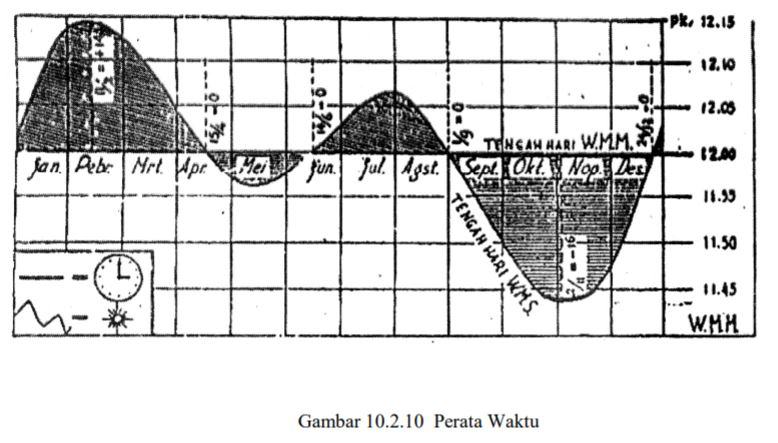
\includegraphics[width=1\textwidth]{figures/sejarahwaktu_Capture.JPG}}
	\caption{gambar Perata Waktu.}
	\label{sejarahwaktu_Capture}
	\end{figure}

 Dari gambar \ref{sejarahwaktu_Capture} kita dapat mengetahui pula bahwa sekitar bulan Januari, Februari
 Maret, Juli, dan Agustus matahari sebenernya lebih lambat sampai titik Kulminasi atasnya,
 sehingga sore lebih lama terangnya.
 
	Contoh: Pada tanggal 2 November jam ditangan kita (waktu matahari menengah) 
	menunjukkan pukul 12.00, tetapi Matahari di langit masih belum tiba di titik Kulminasi 
	Atasnya, baru -16 menit kemudian hal itu terjadi, yaitu pada pukul 11.44 waktu matahari 
	menengah. Sebaliknya, pada bulan Oktober, November, dan Desember matahari menengah 
	lebih lambat daripada matahari sebenarnya. Pagi hari Matahari telah terbit sedangkan 
	jam kita masih menunjukkan kurang dari pukul 06.00. Pada sore harinya pukul 06.00 sudah
	gelap. Hal ini terjadi pada sekitar khatulistiwa (termasuk di Indonesia), 
	di daerah-daerah sedang dan kutub tentunya berbeda.
	
\subsection{Greenwhich Mean Time(GMT)}
Greenwich Mean Time (GMT) adalah tempat yang menjadi
 patokan waktu dunia berada. Jika ditentukan dengan penentuan waktu GMT lebih mudah kita
 dapat menghitung waktu-waktu di seluruh permukaan Bumi. Bagi daerah yang
 berada di belahan barat (meridian barat) waktu setempat adalah waktu GMT
 ditambah dengan hasil kali perbedaan meridian dengan 4 menit sedangkan daerah
 yang berada di belahan timur (meridian timur) waktu setempat adalah waktu GMT
 dikurangi dengan hasil kali antara selisih meridian dengan 4menit. 
 cara perumusannya dengan menggunakan:
					LMT = GMT +(M.4)
			(Dardjosoemartp, dkk.,1991: 445)
			
	LMT = Local Mean Time / Waktu Setempat 
GMT = Greenwich Mean Time / waktu GMT
 + = + bila di BB dan – bila di BT 
(M.4) = meridian (bujur) x 4 menit

\section{Waktu Standar}
\paragraph{Tempat-tempat yang terletak pada garis meridian yang sama, mempunyai waktu yang sama.
 Jika demikian, seluruh permukaan Bumi terdapat 360 waktu yang bedanya 4 menit.
 Hal ini tentu rumit dalam kehidupan sehari-hari. Oleh sebab itu, disepakatilah untuk
 membagi permukaan Bumi atas 24 daerah waktu saja yang disebut waktu standar.}
 
 \paragraph{Waktu standar disebut juga Zone Time, yaitu waktu yang ditetapkan setiap 
 selisih 150 adalah 60 menit (1 jam) dengan lingkup daerah yang berada pada 00 – 150
 atau 150 – 300 , dan seterusnya baik di Bujur Timur maupun Bujur Barat.}
 
 Kongres Internasional memutuskan tentang garis-garis meridian (International Meridian Conferense) 
 di Washington menetapkan waktu standar dunia yang dibagi menjadi 24 daerah berdasarkan
 perbedaan meridian 150 . Setiap daerah mempunyai selisih waktu 1 jam.
 Akan tetapi berdasarkan pembagian wilayah kepemerintahan atau kontinen (pulau/benua)
 maka ada sedikit pergeseran. Batas yang terdapat pada 1800 BT dan 1800 BB berupa garis
 yang berkelok-kelok. Perhatikan gambar \ref{sejarahwaktu_Capture1} di bawah ini:
 
 \begin{figure}{ht}
 \centerline{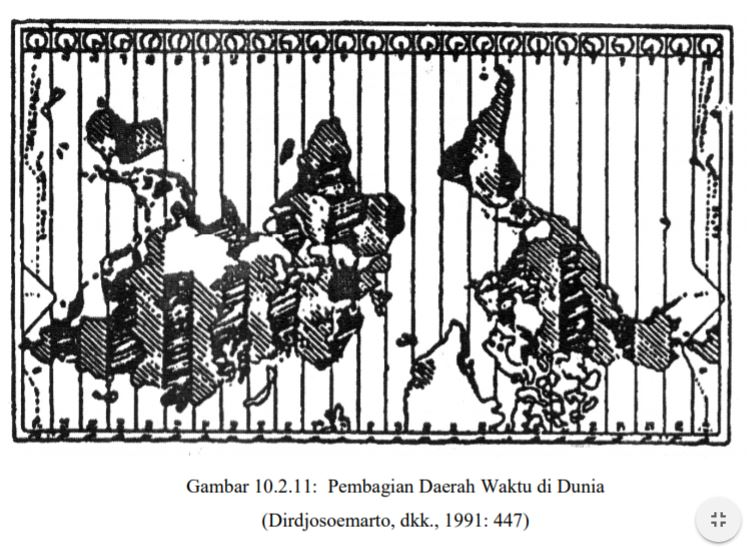
\includegraphics[width=1\textwidth]{figures/sejarahwaktu_Capture1.JPG}}
 \caption{gambar Pembagian Daerah Waktu di Dunia.}
 \label{sejarahwaktu_Capture1}
 \end{figure}
 
 
Setiap negara mempunyai pembagian daerah waktu yang berbeda-beda karena letak pada meridianya berbeda. 
 Indonesia terletak antara 950 BT – 1410 BT. Oleh karena Indonesia mempuyai rentang meridian 1410 – 950 = 460 , 
 maka Indonesia di bagi menjadi 3 daerah waktu, yakni Waktu Indonesia bagian Barat (WIB),
 u Indonesia bagian Tengan (WITA), dan Waktu Indonesia bagian Timur (WIT) dengan selisih
 satu jam. Untuk lebih jelasnya,  perhatikan gambar \ref{sejarahwaktu_Capture2} di bawah.
 
 \begin{figure}{ht}
 \centerline{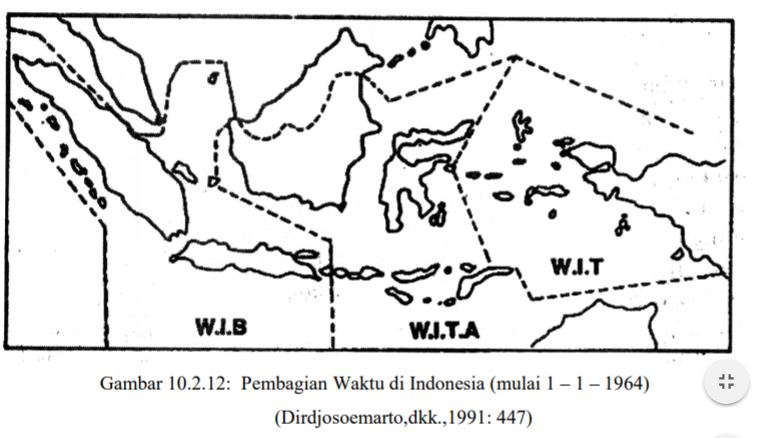
\includegraphics[width=1\textwidth]{figures/sejarahwaktu_Capture2.JPG}}
 \caption{gambar Pembagian Waktu di Indonesia.}
 \label{sejarahwaktu_Capture2}
 \end{figure}
 

Indonesia mempunyai tiga meridian standar, yaitu meridian 1050 BT untuk daerah WIB, 
 1200 BT untuk daerah WITA, dan 1350 untuk WIT .  Dengan demikian waktu lokalnya (LMT) 
 masing-masing adalah waktu Greenwich 
 ditambah 105/15 untuk WIB, 120/15 untuk WITA, dan 135/15 untuk WIT .
 Jika waktu GMT pukul 12.00, maka: WIB = 12.00 + (105/15 = 7) yaitu pukul 19.00,
 WITA = 12.00 + (120/15 = 8) yaitu pukul 20.00, 
 dan WIT = 12.00 + (135/15 =9) yaitu pukul 21.00 (Hidayat,B.,1978: 42).
 \end{document}


\chapter[Sejarah Penanggalan]
{Pengantar\\ Sejarah  Penanggalan}
%Define sejarah penanggalan,bulan dan tahun
%kelompok 4 D4 TI-2D
%Ayu Permata Sari        1154022
%Librantara Erlangga     1154071
%Martin Luter Zega       1154120
%Putri Aulia Ramadhanie  1154096
%Ryan Hafizh Herdiana    1154067
%Copyright (c) 2017 Copyright Holder All Rights Reserved.


\section{Sejarah penanggalan}
  Penanggalan merupakan salah satu sebuah mahakarya yang bisa ditemukan oleh umat manusia. Manusia mempelajari dan memanfaatkan alam [Matahari,Bulan dan Bintang] untuk menghitung pergantian tanggal,bulan dan juga tahun.
umumnya penanggalan digunakan untuk mengetahui waktu yang telah dilewati oleh umat manusia. Adanya sistem penanggalan ini membuat manusia dapat mengingat seluruh kejadian dan pristiwa yang terjadi di dunia ini.
Menurut artikel dari setyanto berdasarkan benda langit yang digunakan sebagai dasar perhitungan sistem penanggalan dapat dikategorikan menjadi 3 kelompok yaitu:\cite{setyanto2015kriteria}

  \subsection{Solar calendar/Kalender Surya}
    Kalender surya menggunakan pergerakan bumi mengelilingi matahari sebagai acuannya.Sistem kalender surya ini biasa digunakan oleh orang-orang eropa. Beberapa contoh kalender yang menggunakan sistem ini yaitu:

    \subsubsection{Julian calendar/Kalender Julian}
      Kalender julian merupakan contoh kalender yang menerapkan sistem surya menurut artikel dari rachmanplanet\cite{rachmanplanet}.Kalender ini telah digunakan bahkan 45 tahun sebelum masehi.
    Awalnya ketika Julius Caesar memimpin pemerintahn romawi terjadi kekacauan  pada perhitungan kalender yang menyebabkan Julis Caesar saat itu mengakhirinya dengan membuat perhitungan kalender sendiri dengan ketentuan:
      1)Satu tahun ditetapkan 565,25 Hari
      2)Tahun biasa, yaitu tiga tahun berturut-turut yang harinya berjumlah 365 Hari
      3)Tahun Kabisat, yaitu tahun keempat ditambah satu hari menjadi 366 Hari.Tambahannya dilakukan pada bulan februari yang jika pada tahun biasa 28 hari pada tahun kabisat ini menjadi 29 hari
      4)Titik permulaan musim semi/bunga ditetapkan pada tanggal 24 Maret
      5)Permulaan tahun ditetapkan pada tanggal 1 Januari (Sebelumnya awal tahun ditetapkan pada tanggal 24 Maret)
    Meskipun kalender julian sudah sangat baik namun ternyata masih terdapat cacat pada kalender tersebut.
    Sebelum orang romawi menggunakan kalender julius caesar, orang romawi sudah menggunakan nama-nama bulan seperti:
    \begin{enumerate}
      \item  Martius     = 31 hari
      \item  Aprilis     = 29 hari
      \item  Majus       = 31 hari
      \item  Junius      = 29 hari
      \item  Quintilis   = 31 hari
      \item  Sextilis    = 29 hari
      \item  September   = 29 hari
      \item  October     = 31 hari
      \item  November    = 29 hari
      \item  Dcember     = 29 hari
      \item  Januarius   = 29 hari
      \item  Februarius  = 28 hari
    \end{enumerate} 

    \subsubsection{Gregorian calendar/Kalender Gregorius}
      Pada tahun 1582 Masehi Paus Gregorius menyaksikan musim semi/bunga pada tanggal 11 maret,bukan lagi pada tanggal 24 maret seperti pada kalender julian.Kemudian paus gregorius memperbaiknya dengan cara:
      1)Musim semi/bunga ditetapkan pada tanggal 21 Maret
      2)Tahun biasa menjadi 365 hari dan tahun kabisat menjadi 566 hari
      Kalender gregorius lebih dikenal dengan nama kalender masehi yang jumlah hari pada setiap bulan dan pentapan awal tahun seperti yang digunakan kalender umumnya saat ini.Kalender masehi dimulai dari tanggal 1 januari
      tahun 1, pukul 00.00.Penamaan bulan pada kalender gregorius yang digunakan hingga sekarang:
      \begin{enumerate}
        \item  January   = 31 hari
        \item  February  = 28/29 hari
        \item  March     = 31 hari
        \item  April     = 30 hari
        \item  May       = 31 hari
        \item  June      = 30 hari
        \item  July      = 31 hari
        \item  August    = 31 hari
        \item  September = 30 hari
        \item  October  = 31 hari
        \item  November = 30 hari
        \item  December = 31 hari
      \end{enumerate}

  \subsection{lunar calendar/Kalender candra}
    \ref{Kalender_2015}
    \begin{figure}[ht]
    \centerline{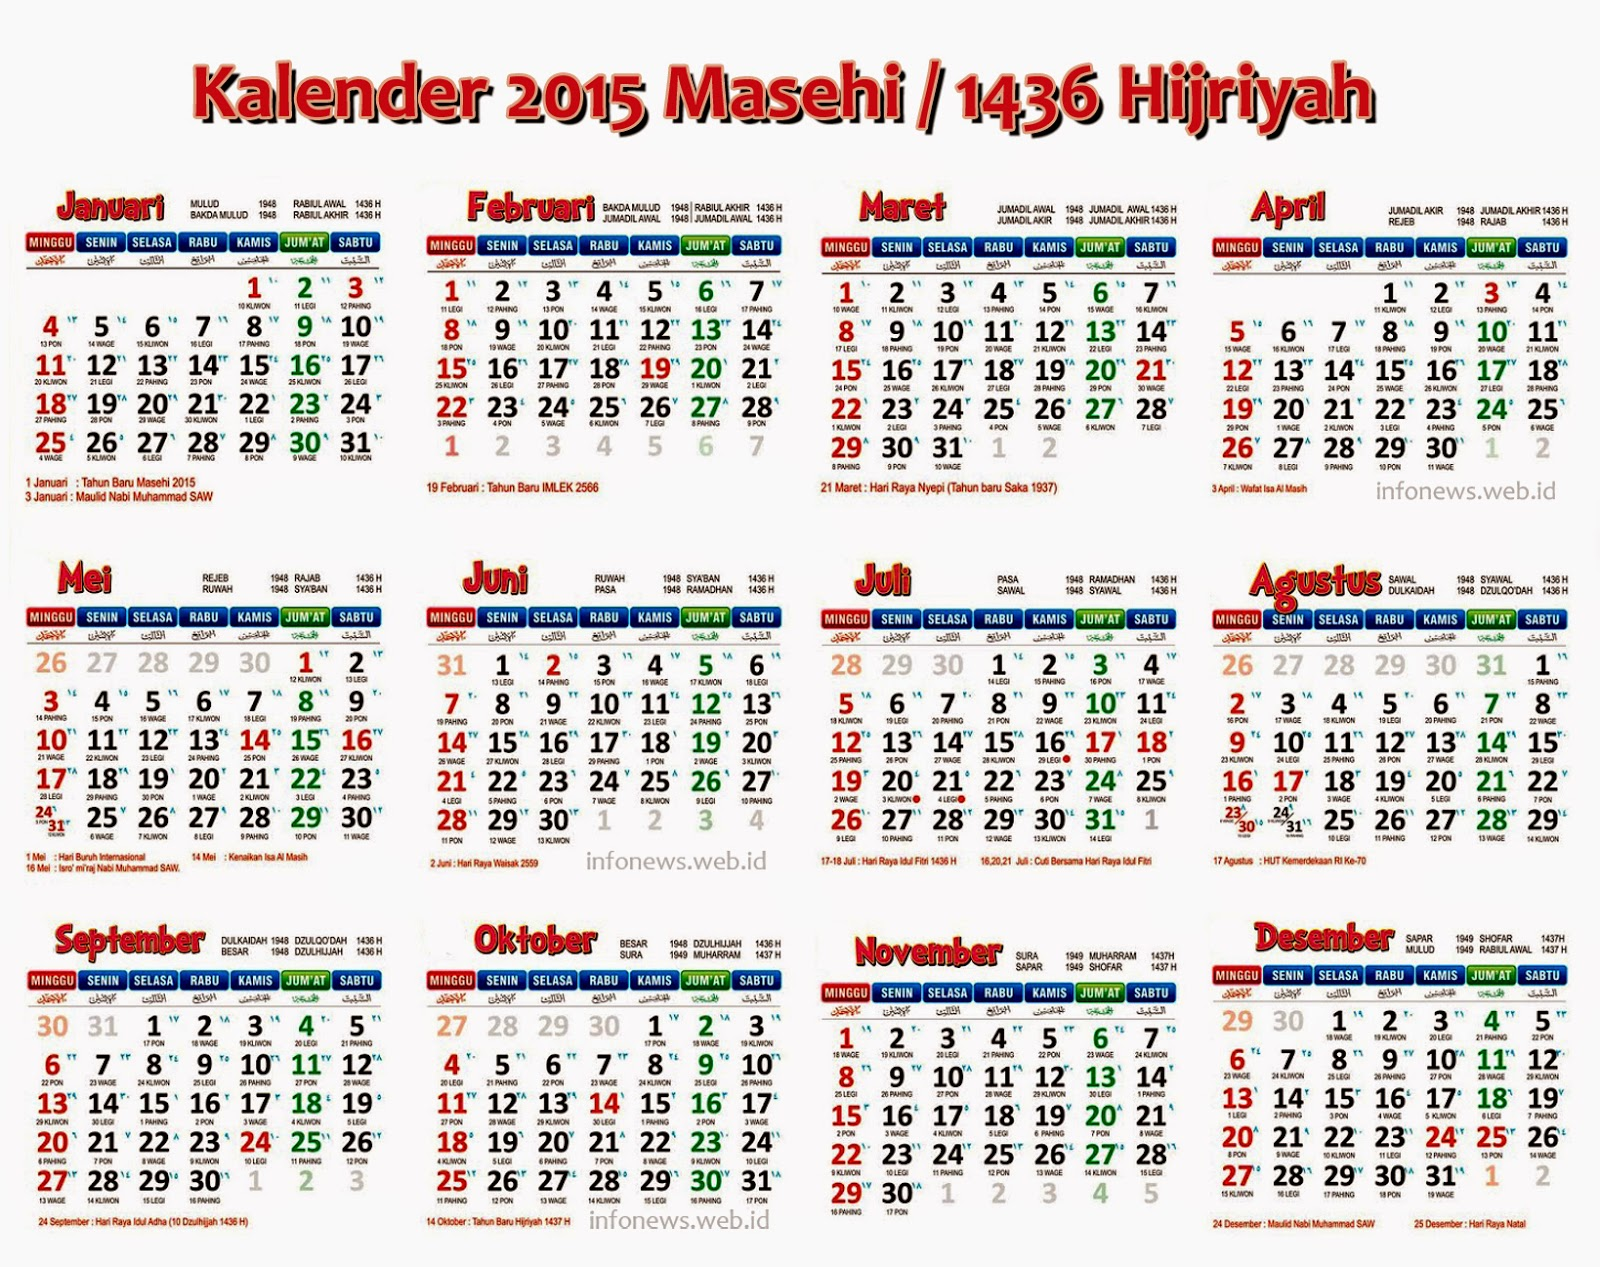
\includegraphics[width=1\textwidth]{figures/Kalender_2015.JPG}}
    \caption{Kalender tahun 2015 Masehi / 1436 Hijriyah.}
    \label{Kalender_2015}
    \end{figure}
    Pembahasan kelender hijriah terkait dengan sistem penanggalan yang berpedoman pada pergerakan Bulan tampak dari Bumi yaitu ketika Matahari dan Bulan yang berada pada posisi bujur astronomi yang sama. Konjungsi merupakan pergerakan pada posisi Bulan dan Matahari yang terlah disepakati sebagai batas penentuan secara astronomis pada kelender Hijriah.
  Bulan yang berkonjungsi searah dengan Matahari akan tampak gelap pada permukaannya ketika dilihat dari Bumi dengan bentuk cahaya sabit kecil. Bulan baru adalah piringan kecil Bulan yang muncul setelah mengalami satu putaran penuh pada fase Bulan mengelilingi Bumi.
  Kemunculan hilal (bulan baru) merupakan penentuan awal bulan dalam Kelender Hijriah di Indonesia, terkhusus pada bulan Ramadhan, Syawal, dan Zulhijah.Kalender merupakan sistem pengorganisasian waktu yang berfungsi sebagai penanda perhitungan dalam jangka panjang. Kelender hijriah termasuk jenis kelender yang penanggalannya berpatokan pada Bulan ketika mengorbit kepada Bumi.
  Perbedaan antara tahun syamsiah dan tahun kamariah yaitu umur hari dalam satu tahun yang 11 hari juga berbeda dalam penentuan awal perhitungan hari. Penanggalan kamariah memiliki perhitungan yang dimulai sejak terbenamnya Matahari dan berakhir ketika Matahari terbenam pada hari esoknya.
  Sistem penanggalan Islam atau kalender hijriah adalah sistem penanggalan yang memiliki dua belas bulan, dimulai sejak Bulan baru hingga penampakan bulan baru berikutnya berkisar selang waktu antara 29 sampai 30 hari. Rovolusi bulan mengililingi bumi memiliki bentuk lintasan yang elips dengan kecepatan tempuh total dalam satu tahun adalah 354 hari 48 menit dan 34 detik.
  Bulan sebagai salah satu komponen penting dalam penanggalan kamariah yakni merupakan satelit tunggal yang dimiliki Bumi. Bulan memiliki 3 pergerakan, diantaranya pergerakan rotasi atau Bulan berputar pada porosnya, revolusi terhadap bumi dan revolusi bersamaan dengan bumi terhadap matahari.

    \subsubsection{Sejarah Kalender Hijriyah}\cite{setyanto2015kriteria}
      Pada saat Sebelum peristiwa haji Wada’ yang dilaksanakan oleh Nabi dan kaum Muslimin, sistem penanggalan masyarakat Arab di Makkah kala itu masih menggunakan konsep penanggalan al-Nasī’. Keberadaan istilah waktu al-Nasī’ tersebut telah mempersulit untuk merunutkan fenomena/peristiwa yang terjadi sebelum haji Wada’.
    Hal ini dikarenakan aturan penggunaan waktu al-Nasī’ tidak berjalan dengan baik. Bangsa Arab dikenal sering memundur dan memajukan kegiatan-kegiatan yang dilakukan pada bulan-bulan Haram sesuai dengan kebutuhannya.4 Hal inilah yang menjadikan penanggalan masyarakat Arab sebelum Haji Wada’ dapat dikatakan tidak konsisten.
    Maksud istilah waktu al-Nasī’ (waktu pengunduran) yaitu diundurnya waktu untuk melaksanakan suatu kegiatan pada waktu tertentu. Salah satunya adalah pengunduran waktu ibadah haji oleh masyarakat Arah ketika itu. Mereka terkadang melaksanakan ibadah haji pada waktunya, terkadang pula pada bulan Muharam, Ṣafar, dan bulan-bulan lainnya di antara dua belas bulan.
    Dampaknya, adalah hal-hal yang mereka yang biasanya dilakukan pada bulan-bulan haram menjadi terabaikan. Hal ini dikarenakan pada saat mereka sedang melaksanakan ibadah haji, mereka bertemu dengan pembunuh ayah mereka, atau bertemu dengan pembunuh sanak saudara mereka, yang menyebabkan mereka membalas dendam pada waktu tersebut.
    Padahal Allah telah menerangkan bahwa melakukan amalan-amalan saleh pada bulan-bulan tersebut merupakan sebesar-besarnya pahala. Sebaliknya, perbuatan zalim yang dilakukan pada saat itu seburuk-buruknya kesalahan, bahkan menambah kekafiran.
    Namun demikian, konsep al-Nasī’ dimaksudkan untuk menyesuaikan fase Bulan dengan perubahan musim yang diakibatkan oleh posisi dan gerak Matahari di Jazirah Arab.Sehingga dapat dikatakan penanggalan masyarakat Arab ketika itu termasuk menggunakan sistem Penanggalan Matahari-Bulan (Kala Surya-Chandra).
    Meski demikian, Nabi Muhammad beserta umat Islam kala itu mengikuti kalender yang sedang berjalan. Sehingga dapat dikatakan seluruh hidup Nabi Muhammad berpuasa dalam sistem penanggalan yang ditetapkan oleh bangsa Quraisy. Nabi tidak membuat sistem penanggalannya sendiri.Turunnya QS.
    al-Taubah [9]: 36-37, yang melarang penggunaan yaum al-Nasi’ (waktu pengunduran) telah mengubah sistem penanggalan masyarakat Arab dari sistem Lunisolar Calendar menjadi sistem Lunar Calender. hal Inilah yang menjadi awal mula atau kelahiran sistem penanggalan Islam yang berbasis pada pergerakan Bulan dalam mengelilingi Bumi.
    Hingga saat ini belum diketahui dengan baik bagaimana praktek penanggalan Islam pada zaman sahabat. Namun, diyakini penanggalan Islam pada masa itu didasarkan pada kesaksian ru’yat al-hilāl. Adapun proses bagaimana praktek penanggalan Hijriyah sejak berubahnya sistem penanggalan tersebut pada dasarnya dapat ditelusuri melalui sejarah, sebagaimana yang telah dilakukan oleh Saleh al-Saab dari King Abdul’aziz City for Science and Technology (KACST), Riyadh.
    Praktek penanggalan Islam kemudian disempurnakan melalui konsep penanggalan yang dirumuskan pada zaman Umar bin Khaṭṭab. Melalui sidang para sahabat rasulullah, ditetapkanlah perhitungan tahun dalam penanggalan kekhalifahan, dimulai sejak hijrahnya Nabi Muhammad dari Mekkah ke Madinah.
    Penetapan tahun hijrahnya Nabi sebagai tahun pertama tersebut merupakan usulan dari Sahabat ‘Ali bin Abī Ṭālib.11 Oleh karena itu, penanggalan kekhalifahan Islam dikenal sebagai penanggalan Hijriyah, dengan bulan Muharam sebagai bulan pertama dalam penanggalan tersebut. Hal tersebutlah yang telah umum berlaku di masyarakat Arab ketika itu.
    Sama halnya dengan penanggalan Masehi yang digunakan saat ini, penanggalan Hijriyah pun pada zaman sahabat ditetapkan berdasarkan perhitungan matematis. Jumlah hari yang digunakan senantiasa tetap setiap bulannya. Meskipun demikian, hal-hal yang terkait dengan pelaksanaan ibadah kaum Muslimin kala itu tetap mengikuti ketentuan yang telah diajarkan oleh Nabi Muhammad.
    Oleh karenanya, penanggalan pada kalender Hijriyah yang telah ditetapkan merupakan penanggalan Administrasi Negara.Seiring dengan perkembangan pemahaman dan pengetahuan, saat ini fungsi penanggalan Hijriyah sebagai penanggalan sosial menjadi satu kesatuan dengan fungsinya sebagai penanggalan ibadah. Hal inilah yang dilihat secara subyektif sebagai kisruh sistem penanggalan Hijriyah.
    Maka dari itu, untuk mengurai permasalahan pada tahap awal adalah dengan melepaskan fungsi ibadah dari sistem penanggalan Hijriyah.Namun, aturan ibadah tetap menjadi acuan dalam penyusunan kalender Hijriyah, sebagaimana yang telah dipraktekkan oleh sahabat. Dalam beribadah terdapat kesepakatan pada proses pencapaian kesatuan dalam beribadah yaitu dapat diawali dengan menyepakati penggunaan kalender tunggal yang digunakan bersama, sedangkan pelaksanaan ibadah dikembalikan kepada masing-masing.Berikut adalah nama bulan dan hari pada kalender hijriyah berdasarkan pada hisab urfi:
    \begin{enumerate}
        \item Muharram      = 30 hari
        \item Shafar        = 29 hari
        \item Rabiul Awwal  = 30 hari
        \item Rabiul Akhir  = 29 hari
        \item Jumadil Awwal = 30 hari
        \item Jumadil Akhir = 29 hari
        \item Rajab         = 30 hari
        \item Shaban        = 29 hari
        \item Ramadhan      = 30 hari
        \item Syawal        = 29 hari
        \item Dzulka'idah   = 30 hari
        \item Dzhulhijjah   = 29/30 hari
    \end{enumerate}

  \subsection{lunisolar calendar/kalender suryacandra}
      Menurut wicaksono dalam artikelnya Lunisolar kalender merupakan sistem kalender candra yang disesuaikan dengan matahari \cite{wicaksono2008ta}.Karena kalender candra dalam 1 tahun mempunyai 11 hari lebih cepat dari kalender surya, maka dalam kalender suryacandra memiliki bulan interkalasi(bulan tambahan/bulan ke -13)setiap 3 tahun, agar kembali seusai dengan perjalanan matahari.
    beberapa contoh kalender yang mengacu pada sistem suryacandra adalah kalender imlek/cina,saka,dan budhha. Semua kalender tersebut tidak ada yang sempurna ,karena jumlah hari dalam satu tahun itu tidak bulat,dan untuk memperkecil error itu maka dibuat kesepakatan sehari lebih panjang atau terdapat bulan tambahan dalam kalender cina pada tahun kabisat\cite{wicaksono2008ta}.
    Pada kalender surya, pergantian hari terjadi tengah malam dan awal setiap bulan (tanggal 1) yang tidak tergantung pada posisi bulan dan pada kalender candra dan suryacandra pergantian hari terjadi ketika matahari terbenam dan awal setiap bulan adalah saat konjungsi(imlek,sakka,budhha) atau dalam hijriyah saat munculnya hilal.




\chapter[Bangun Ruang]
{Pengantar\\ Bangun Ruang}
%kelompok 2
%Achmad Fatahillah(1154004)
%Ilga Anne Tri J.S(1154045)
%Maulyanda(1154008)
%Mefi Frinkazela Nikica(1154073)
%Simon Sorba Manangi(1154019)
	
\section{Bangun Ruang}
Bangun ruang merupakan suatu bagian ruang yang dibatasi oleh himpunan titik-titik yang terdapat pada seluruh permukaan bangun tersebut. 
Permukaan bangun tersebut disebut sisi. Bangun ruang memiliki tiga unsur, yaitu 
panjang : merupakan suatu dimensi dalam benda yang menunjukkan sebuah jarak antar ujung satu ke ujung lainnya.
lebar   : merupakan lintasan dalam sebuah bidang.
tinggi  : merupakan ukuran sebuah objek yang diukur secara vertikal.
Bangun ruang memiliki volume. Rumus volume umum pada bangun ruang adalah panjang(p) x lebar(l) x tinggi(t).
Tujuan menghitung volume adalah untuk menghitung berapa banyak ruang yang dapat diisi datau ditempati pada suatu objek.

Sisi bangun ruang adalah suatu himpunan pada titik-titik yang terdapat pada permukaan atau yang membatasi suatu bangun ruang tersebut \cite{umami2013eksperimentasi}

Dalam memilih model untuk permukaan atau sisi, dapat karena kedudukan semua unsur bangun ruang dapat diamati untuk dialihkan dalam gambar\cite{suharjana2008mengenal}. 
Ada beberapa contoh benda yang mewakili gambar bangun ruang\ref{contohbangun}.
\begin{figure}[ht]
    \centerline{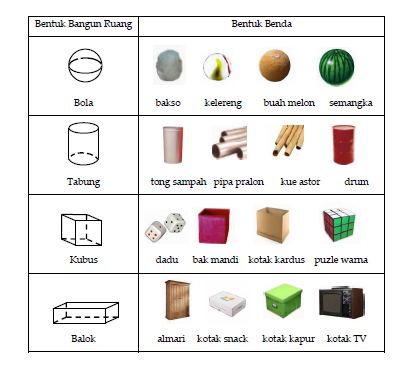
\includegraphics[width=1\textwidth]{figures/contohbangun.png}}
    \caption{beberapa kumpulan gambar yang termasuk dalam bangun ruang}
    \label{contohbangun}
    \end{figure}
 
Bangun ruang sering  disebut bangun 3 dimensi karena memiliki 3 komponen utama sebagai berikut.
1.Sisi  merupakan bidang pada bangun ini memiliki ruang yang membatasi antara bangun ruang dengan ruangansekitarnya 
2.Rusuk merupakan pertemuan antar dua sisi yang berupa ruas garis pada bangun.
3.Titik sudut merupakan titik hasil pertemuan rusuk yang berjumlah tiga atau lebih

Unsur-unsur Bangun Ruang Sisi,rusuk,dantitiksudut. Sebagai mengingatkan bahwa setiap model bangun ruang pasti memiliki sisi, rusuk, dan titiksudut , kecuali bola, tabung,dankerucut.
Bangun ruang, limas, prisma, dan sisi, rusuk, titiksudut serta dikembangkan pada diagonalsisi,diagonalruang, dangaris-garis sejajar.
menggunakan model bangun ruang yang transparan  melihat sisi bangun ruang tersebut, model transparan, bangun ruang dengan model transparan ini juga dapat untuk menggambar bangun ruang, karena semua unsur bangun ruang dapat diamati untuk dialihkan dalam gambar. Setelah mengamati, 
menelusuri, dan memahami unsur-unsur bangun ruang tersebut.

Jenis-Jenis Bangun Ruang yang umum dikenal adalah:
1.  kubus merupakan bangun ruang yang dibatasi oleh enam buah bidang sisi berbentuk persegi dengan ukuran yang sama.
2.balok yaitu bangun ruang dengan dibatasi dengan enam bidang sisi yang memiliki bentuk persegi panjang yang setiap sepasang-sepasang sejajar dan sama ukurannya.
3.prisma yaitu adalah sebuah bangun ruang yang diberikan batas oleh dua buah daerah segitiga yang sejajar sehingga tiga daerah persegi panjang tersebut yang saling berpotongan menurut garis-garis yang sejajar.
4.limas merupakan bangun ruang yang dibatasi leh sebuah daerah segiempat dan empat daerah segitiga yang mempunyai satu titik sudut persekutuan.
5.kerucut merupakan bangun ruang yang dibatasi oleh sebuah bidang lengkung yang simetris terhadap porosnya yang melalui titik pusat lingkaran tersebut.
6.tabung merupakan bangun ruang yang setiap sisinya dibatasin dengan dua bidang lingkaran yang sama-sama sejajar dan sama-sama ukurannya dan satu buah bidang 
     yang memiliki jarak sama jauhnya ke arah poros dan sisi yang simetris ke arah porosnye itu akan memotong dua daerah bidang lingkaran tepat di kedua lingkaran itu .
7.Bola
Jenis-Jenis Bangun Ruang yang umum dikenal adalah dan di dalam kehidupan sehari hari:
1.   Kubus    : dadu, rubik
2.   Balok    : lemari, tv
3.   Prisma    : atap rumah, tenda pramuka
4.   Limas    : piramida, monas
5.   Kerucut: nasi tumppeng yang berbentuk kerucut
6.   Tabung    : minuman kaleng, gas elpiji
7.   Bola    : bola basket, bola tenis

Dalam pembelajaran bangun ruang dan unsur-unsurnya maka harus DIPERKENALKAN model-model bangun ruang, misalnya model kubus, balok, prisma, limas, tabung, kerucut, dan bola. apabila diambil contoh-contoh dari bendabenda yang dapat ditemukan dalam kehidupan sehari-hari, misalnya kaleng roti untuk menunjukkan tabung, tumpeng untuk menunjukkan kerucut dan seterusnya. Yang tidak transparan, transparan dan kerangka. Hal tersebut akan lebih memudahkan dalam pemahamanbangun ruang dan unsur unsurnya, menentukan sifat sifat bangun ruang, serta dapat menterjemahkan gambar dalam bangun ruang dans ebaliknya.
Contoh di bidang bangun ruang yaitu dalam bidang geometri  materi matematika bentuk bangun datar 2D maupun bangun ruang 3D. 
Manfaat yang dapat diperoleh dari penelitian memberikan gambaran 3D dari pemodelan bangun geometri halnya alat perga dalam membangun siswa dalam mempelajari bentuk bangun geometri.
Bangun ruang dalam bentuk geometris yang terdiri atas tiga dimensi( panjang lebar dan tinggi) bangun ruang yang di bahas di dalam geometri antara lain :
1.    Kubus
2.    Balok 
3.    Prisma
4.    Limas
5.    Tabung
6.    Kerucut
7.    Bola

Kebutuhan di bangun ruang dapat disimpulkan bahwa diperlukan 
1.    Pengertian dan ciri-ciri berapa bangun datar dan bangunan ruangan.
2.    Data rumus luas bangun datar.
3.    Data rumus volum bangun datar dan bangun ruang.

Kebutuhan disini sudah diperoleh dari buku matematika sekolah dasar.

\subsection{Bola} 

\begin{figure}[ht]
    \centering
	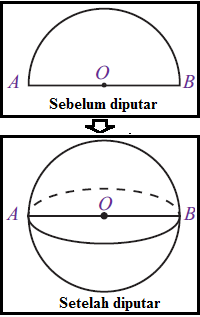
\includegraphics[width=0.5\textwidth]{figures/bola1.png}
    \caption{contoh bola}
    \label{bola1}
\end{figure}

Dalam bangun ruang, bola adalah bangun ruang tiga dimensi yang dibentuk sehingga tak terhingga lingkaran yang berjari-jari sama panjangnya dan berpusat pada satu titik yang sama. Bola merupakan bangun ruang sisi lengkung yang dibatasi oleh satu bidang lengkung.
contoh bangun ruang bola dalam kehidupan sehari-hari adalah dalam sebuah olah raga sepak bola, basket, kasti, bowling, dan sebagai nya. bola dapat menggelinding dan dapat memantul dengan sempurna, karena tidak adanya sudut pada bola. 
Bentuk bumi pun seperti bola, terlihat pada sebuah dokumentasi dari pesawat ruang angkasa, maupun dalam hal perjalan lurus, pasti akan kembali lagi ketempat kita memulai perjalanan.
Bola dapat dibentuk dari bangun setengah lingkaran yang diputar sejauh 360° pada garis tengahnya. 
Pada gambar  \ref{bola1} merupakan setengah lingkaran dengan diameter AB  tersebut dan dapat diputar satu putaran dengan diameter sebagai suatu sumbu putar maka akan tampak gambar seperti di bawahnya yang disebut bangun ruang.


Bola merupakan bangun ruang sisi lengkung (BRSL) yang terjadi dari tumpukan empat buah lingkaran \ref{sisilengkung}.
\begin{figure}[ht]
    \centering
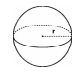
\includegraphics[width=0.25\textwidth]{figures/sisilengkung.png}
    \caption{contoh sisi lengkung}
    \label{sisilengkung}
    \end{figure} 
Keempat lingkaran ini dinamakan kulit bola. Kulit bola berada pada sisi luar bola atau mengelilingi bola \cite{nurfarikhin2010hubungan}.

Rumus bola:

a) Luas permukaan
 \begin{equation}
     L = 4 \pi r^2 \,
\end{equation}
b) Volume
\begin{equation}
     V = \frac{4}{3}\pi r^3
\end{equation}
\subsubsection{Sifat-sifat pada bola} 
a) Memiliki 1 sisi yang berbentuk bidang lengkung (selimut bola) 
b) Tidak memiliki rusuk 
c) Tidak memiliki titik sudut
 
Adapun unsur-unsur bangun ruang bola yang terdapat pada gambar \ref{unsurbola} sebagai berikut.
\begin{figure}[ht]
    \centerline{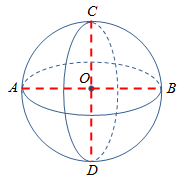
\includegraphics[width=1\textwidth]{figures/unsurbola.png}}
    \caption{contoh usur bola}
    \label{unsurbola}
    \end{figure}
1) Titik pada titik O dinamakan titik pusat bola.
2) Ruas garis pada OA disebut sebagai jari-jari pada bola. Sebutkan jari-jari pada bola lainnya.
3) Ruas garis pada CD diberi nama sebagai diameter pada bola. Jika kita amati, ruas pada garis AB tersebut merupakan diameter bola. AB dapat pula disebut sebagai tinggi bola.
4) Sisi bola merupakan kumpulan titik - titik yang mempunyai jarak yang sama terhadap titik O. Sisi tersebut dinamakan selimutatau kulit bola.
5) Ruas garis ACB dinamakan tali busur bola.
6) Ruas-ruas pada garis selimut bola yaitu ACBDA dinamakan garis pelukis bola.

\subsubsection{Konsep luas permukaan Bola}
Penentuan luas sisis (permukaan) bola dapat kita lakukan dengan sebuah percobaan archimedes, yaitu:
Sebuah bola menempati sebuah tabung yang memiliki diameter dan tinggi tabung sama tepat dengan 
yang dimiliki oleh diameter bola, maka luas bola itu sama dengan luas selimut tabung \ref{bolatabung}.
\begin{figure}[ht]
    \centerline{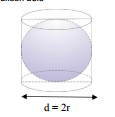
\includegraphics[width=1\textwidth]{figures/bolatabung.png}}
    \caption{sebuah bola yang terdapat dalam tabung, untuk mengukur luar permukaan tabung}
    \label{bolatabung}
    \end{figure} 
Berdasarkan gambar maka diperoleh :

Luas selimut tabung 
\begin{equation}
					L= 2 pr. T
                    = 2pr. 2r
                    = 4pr2
\end{equation}
            
\subsubsection{Konsep volume bola}
Apabila kita mengisi air ke dalam bangun bola secara penuh 
kemudian menuangkannya ke bangun ruang tabung maka air yang diperoleh adalah 2/3 bagian dari volume bangun ruang tabung tersebut. 
Dengan ketentuan bahwa kedua bangun tersebut memiliki jari-jari yang sama sehingga diperoleh:
\begin{equation}
Volume bola = 2/3 . volume tabung(silinder)
            = 2/3 . (pr2 . 2r)
\end{equation}

\subsubsection{Asal-usul rumus permukaan bola}
Jika ingin mendapatkan rumus permukaan bola, kita mulai kegiatan berikut ini untuk menguji rumus tersebut.
1. Sediakan sebuah bola berukuran sedang seperti bola sepak atau bola basket.
2. Ukurlah setiap keliling bola tersebut menggunakan benang.
3. Lilitkan benang tersebut pada permukaan setengah bola sampai penuh, seperti gambar \ref{bola2}.
\begin{figure}[ht]
    \centerline{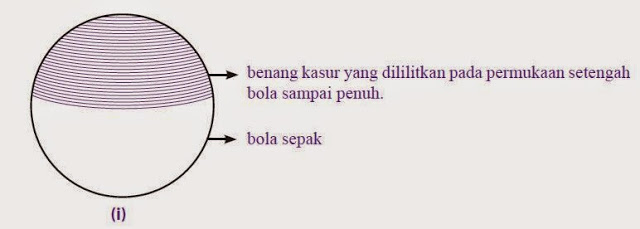
\includegraphics[width=1\textwidth]{figures/bola2.jpg}}
    \caption{gambar bola}
    \label{bola2}
    \end{figure}
4. Buatlah persegi panjang dari kertas karton dengan ukuran panjang sama dengan keliling bola dan lebar sama dengan diameter bola seperti gambar \ref{bola3}.
\begin{figure}[ht]
    \centerline{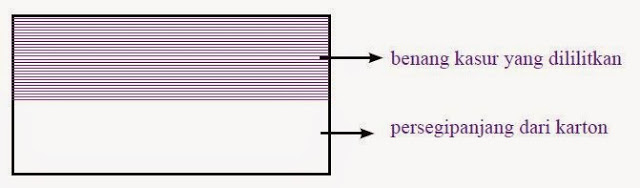
\includegraphics[width=1\textwidth]{figures/bola3.jpg}}
    \caption{beberapa kumpulan gambar yang termasuk dalam bangun ruang}
    \label{bola3}
    \end{figure}
5. Lilitkan benang yang telah digunakan untuk melilit permukaan setengah bola pada persegipanjang yang kamu buat tadi. Lilitkan sampai habis.
6. Jika kamu melakukannya dengan baik, tampak benang tersebut menutupi persegi panjang selebar jari-jari bola (r).
7. Hitunglah luas dari persegi panjang yang telah ditutupi benang tersebut. 
\begin{equation}
Luas permukaan setengah bola = luas persegi panjang
                                           = p × l
                                           = 2πr× r
                                           = 2π r2
\end{equation}

Jadi, luas permukaan bola dirumuskan sebagai berikut :
\begin{equation}
Luas permukaan bola ( L = 4πr2 )
\end{equation}
Keterangan :
L = luas permukaan bola.
r = jari-jari bola.
π = 22/7 atau 3,14

\subsubsection{Asal-usul rumus volume bola}
Cara - cara untuk mengetahui rumus volume bola, dapat dilakukan dengan cara - cara seperti berikut ini : 
1. Siapkan sebuah tempat yang berbentuk setengah bola berjari-jari r (\ref{wadah1}) dan sebuah wadah yang berbentuk kerucut berjari-jari r dan tingginya 2r (\ref{wadah2}).
2. Isikan pasir ke \ref{wadah2} sampai penuh.
3. Pindahkan pasir di dalam \ref{wadah2} ke \ref{wadah1}. Apakah yang terjadi?
\begin{figure}[ht]
    \centerline{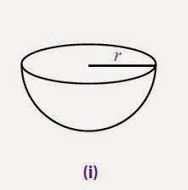
\includegraphics[width=1\textwidth]{figures/wadah1.jpg}}
    \caption{wadah dalam bola}
    \label{wadah1}
    \end{figure}
\begin{figure}[ht]
    \centerline{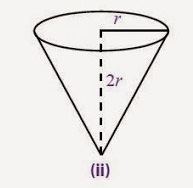
\includegraphics[width=1\textwidth]{figures/wadah2.jpg}}
    \caption{pasir dalam wadah}
    \label{wadah2}
    \end{figure}

Dari cara seperti diatas tersebut, dapat dilihat bahwasanya volume dari pasir yang dituangkan ke dalam wadah setengah bola tidak dapat berubah. Ini berarti, untuk membangun setengah bola, dan kerucut yang berjari-jari sama, dan tinggi kerucut sama dengan dua kali jari-jarinya maka:
\begin{equation}
Volume setengah bola = volume kerucut
1/2 volume bola = 1/3 πr2t
volume bola = 2/3πr2(2r)
                         = 4/3πr3
\end{equation}
Jadi, volume bola tersebut dirumuskan sebagai berikut :
\begin{equation}
Volume bola ( V = 4/3πr3 )
\end{equation}
Keterangan :
V = volume bola.
r = jari-jari bola.
π =22/7 atau 3,14.

Contoh soal :
bola memiliki jari-jari 9 cm, hitunglah volume bola tersebut ?

Jawab :
Diketahui : r = 9 cm
Ditanyakan : volume bola ?
Penyelesaian :
\begin{equation}
V   = 4/3pr3
    = 4/3/ 3 , 14 . (9)3
    = 3.052,08
\end{equation}
Jadi, volume bola tersebut 3.052,08 cm3

\chapter[Diagram Kartesius]
{Pengantar\\ Kartesius}
% Kelompok Diagram Kartesius
% Rahmi Nurdin (1154109)
% Mustari Muammar (1154108)
% Fadillah Firdaus (1154103)

\section{Pengertian Diagram Kartesius}
Diagram Kartesius adalah sistem kooordinat yang terdiri dari dua sumbu yang berisi titik-titik sebagai simbol relasi.
Domain sebagai sumbu horizontal dan kodomain sebagai sumbu vertikal.
Pada koordinat kartesius daerah asal (domain) diletakkan pada sumbu X (sumbu mendatar) dan daerah kawan (kodomain) diletakkan pada sumbu Y (sumbu tegak).
Sedangkan daerah hasilnya merupakan titik (noktah) koordinat pada diagram kartesius. Dari relasi di atas, dapat ditunjukkan diagram kartesiusnya seperti di bawah :
\begin{figure}[ht]
	\centerline{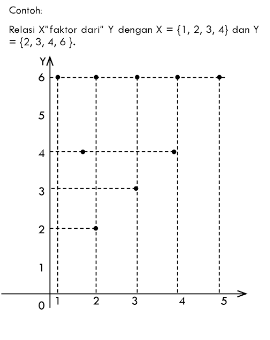
\includegraphics[width=1\textwidth]{figures/rahmi1.PNG}}
	\caption{hubungan antar titik pada diagram kartesius.}
	\label{rahmi1}
	\end{figure}

Diagram Kartesius merupakan suatu bangunan atas empat bagian yang batasi oleh dua buah garis yang berpotongan tegak lurus pada titik-titik (  X, Y ). 
Dimana X merupakan rata-rata dari rata-rata skor tingkat pelaksanaan atau kepuasan konsumen dari sebuah faktor atribut 
dan Y adalah rata-rata skor tingkat kepentingan seluruh faktor atau atribut yang mempengaruhi kepuasan konsumen.
Seluruhnya ada K faktor. Rumus berikutnya yang digunakan adalah :
\begin{figure}[ht]
	\centerline{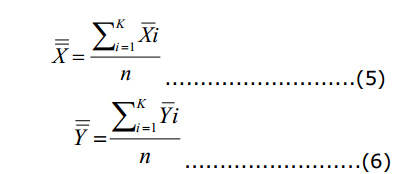
\includegraphics[width=1\textwidth]{figures/rahmi2.PNG}}
	\caption{rumus mencari K faktor.}
	\label{rahmi2}
	\end{figure}

Dimana :K = Banyaknya faktor atau atribut yang mempengaruhi kepuasan konsumen 
Diagram Kartesius	
\begin{figure}[ht]
	\centerline{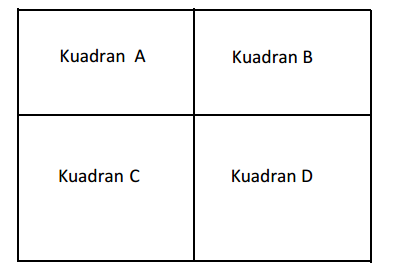
\includegraphics[width=1\textwidth]{figures/rahmi3.PNG}}
	\caption{penentuan kuadran pada diagram kartesius.}
	\label{rahmi3}
	\end{figure}

Gambar 1. Diagram Kartesius



Kuadran A
Pada posisi ini, jika dilihat dari kepentingan konsumen, atribut-atibut produk berada pada tingkat tinggi, tetapi jika di lihat dari kepuasannya, 
konsumen merasakan tingkat yang rendah, sehingga konsumen menuntut adanya perbaikan atribut tersebut.
Kuadran B
Pada posisi ini, jika dilihat dari kepentingan konsumen, atribut-atribut produk berada pada tingkat tinggi, dan dilihat dari kepuasannya, 
konsumen merasakan tingkat yang tinggi juga.
Kuadran C
Pada posisi ini, jika dilihat dari kepentingan konsumen, atribut-atribut produk kurang dianggap penting, tetapi jika dilihat dari tingkat kepuasan konsumen cukup baik.
Namun, konsumen mengabaikan atributatribut yang terletak pada posisi ini.
Kuadran D
Pada posisi ini, jika dilihat dari kepentingan konsumen, atribut-atribut produk kurang dianggap penting, tetapi jika dilihat dari tingkat kepuasanya, konsumen merasa
sangat puas.


\section{Penghitungan Rumus Diagram Kartesius}
\subsection{meghitung rumus, mencari titik}

Kartesius digunakan untuk menentukan tiap titik dalam bidang dengan menggunakan dua bilangan yang biasa disebut koordinat x dan koordinat y.
\begin{figure}[ht]
	\centerline{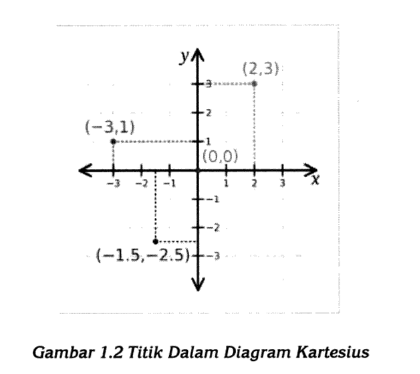
\includegraphics[width=1\textwidth]{figures/rahmi9.PNG}}
	\caption{penentuan titik pada kuadran katesius.}
	\label{rahmi9}
	\end{figure}

Sebuah titik dalam Diagram Kartesius, mengandung dua buah informasi yakni sumbu (x,y), seperti tampak pada Gambar 1.2. 
Yaitu titik (2,3) adalah titik dimana nilai x=2 dan y=3. Daerah ini dikenal dengan kuadran I, dimana nilai x dan y adalah positif.
\begin{figure}[ht]
	\centerline{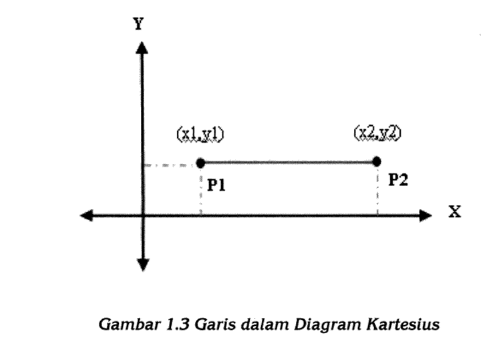
\includegraphics[width=1\textwidth]{figures/rahmi10.PNG}}
	\caption{penentuan garis pada kuadran katesius.}
	\label{rahmi10}
	\end{figure}

Dari dua buah titik diagram kartesius, bisa ditarik menjadi sebuah garis. Artinya pada sebuah garis memiliki titik awal


\section{Contoh Penerapan/Pemetaan Diagram Kartesius}
Tujuan digunakannya diagram kartesius adalah untuk melihat secara lebih terperinci mengenai atribut-atribut yang perlu untuk dilakukan perbaikan. 
Langkahlangkah sebelum memetakan data ke diagram kartesius ini, adalah terlebih dahulu dengan menentukan nilai rata-ratasetiap atribut yaitu X dan Y, 
dimana nilai perhitungannya telah kita peroleh dari perhitung yang dilakukan sebelumnya.
Adapun hasil pembagian setiap atribut pada setiap kuadaran ditampilkan pada gambar 2
\begin{figure}[ht]
	\centerline{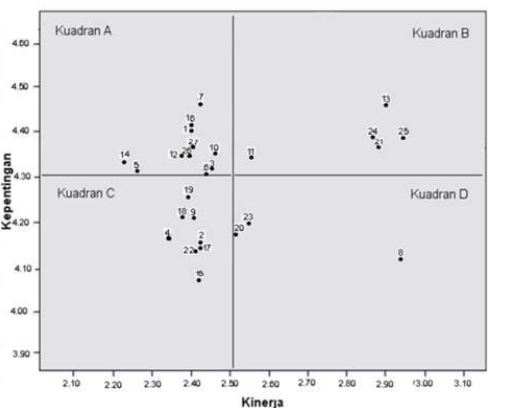
\includegraphics[width=1\textwidth]{figures/rahmi4.PNG}}
	\caption{.}
	\label{rahmi4}
	\end{figure}


Gambar 2. Diagram Kartesius
Setelah dilakukan perhitungan menggunakan diagram kartesius didapat hasil atribut-atribut yang harus diperbaiki adalah atribut yang berada pada kuadran A.
Adapun atribut yang harus diperbaiki pada kuadran A adalah :
Tabel 2 Hasil Perhitungan Diagram Kartesius pada Kuadran A	
\begin{figure}[ht]
	\centerline{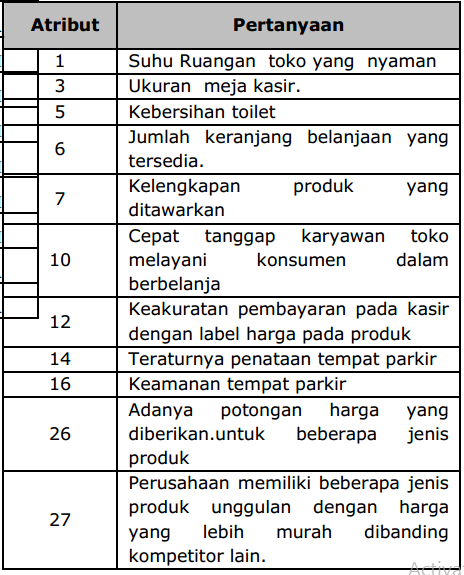
\includegraphics[width=1\textwidth]{figures/rahmi5.PNG}}
	\caption{.}
	\label{rahmi5}
	\end{figure}


Untuk atribut-atribut yang harus dipertahanan oleh pihak perusahaan setelah dilakukannya perhitungan menggunakan diagram kartesius adalah atribut-atribut
yang berada pada kuadran B, karena pada atribut yang berada pada kuadran B dianggap pelanggan sudah dapat memenuhi apa yang mereka inginkan. 
Adapun atribut yang harus dipertahankan dapat dilihat pada
Tabel 3.
Tabel 3. Hasil Perhitungan Diagram Kartesius
pada Kuadran B
\begin{figure}[ht]
	\centerline{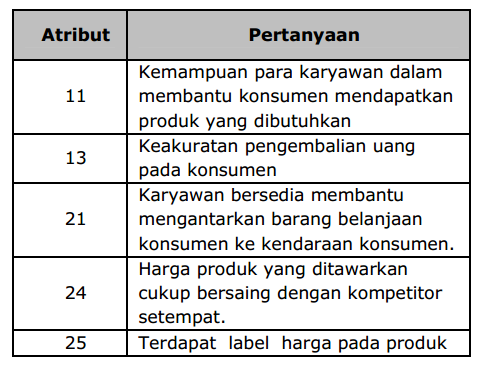
\includegraphics[width=1\textwidth]{figures/rahmi6.PNG}}
	\caption{.}
	\label{rahmi6}
	\end{figure}

Atribut yang memiliki penilaian yang rendah karena atribut-atribut ini kurang dianggap penting oleh pelanggan dan perusahaan juga tidak memberikan pelayanan atau perhatian khusus, 
atribut ini dianggap tidak memberikan dampak yang besar bagi perusahaan.
Adapun atribut-atribut yang berada pada kuadran C dapat dilihat pada Tabel 4.
Tabel 4. Hasil Perhitungan Diagram Kartesius pada kuadran C
\begin{figure}[ht]
	\centerline{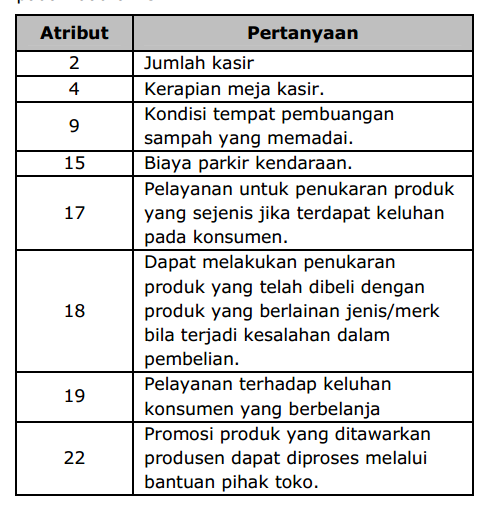
\includegraphics[width=1\textwidth]{figures/rahmi7.PNG}}
	\caption{.}
	\label{rahmi7}
	\end{figure}

Untuk atribut yang ada pada kuadran D adalah atribut yang tidak dianggap penting bagi pelanggan, namun pihak perusahaan memberikan pelayanan yang berlebihan 
sehingga atribut ini dianggap berlebihan.
Adapun atribut yang berada pada kuadran D dapat dilihat pada Tabel 5.
Tabel 5. Hasil Perhitungan Diagram Kartesius
pada Kuadran D	
\begin{figure}[ht]
	\centerline{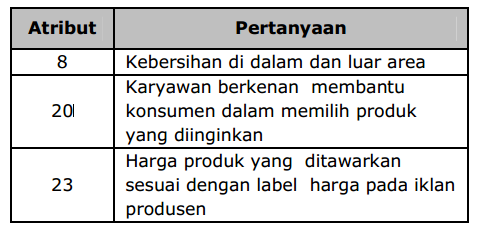
\includegraphics[width=1\textwidth]{figures/rahmi8.PNG}}
	\caption{.}
	\label{rahmi8}
	\end{figure}


Diagram Kartesius
Dari hasil perhitungan yang telah dilakukan sebelumnya, terdapat 17 atribut yang perlu dilakukan perbaikan (Action) danterdapat 10 atribut yang perlu mendapat
perhatian untuk dipertahankan oleh pihak perusahaan (Hold). Diagram Kartesius Dari hasil pemetaan yang dilakukan pada diagram kartesius dapat terlihat beberapa
atribut yang perlu untuk dilakukannya perbaikan dan atribut-atribut perlu untuk dipertahankan oleh pihak perusahaan yang terbagi kedalam kuadran-kuadran (A, B, C
dan D) sesuai dengan tingkat kesesuaian antara tingkat kepentingan pelanggan dan kinerja perusahaan, yaitu dengan tingkat kesesuaian sebesar 58.374.
Adapun hasil pemetaannya adalah sebagai berikut:
Kuadran A
Kuadran A adalah wilayah yang berisikan atribut-atribut yang dianggap penting oleh pelanggan, namun dalam kenyataannya atribut-atribut ini masih belum sesuai
dengan yang diharapkan oleh pelanggan. Dalam hal ini perusahaan perlu melakukan perbaikan sebaik mungkin untuk meningkatkan kepuasan pelanggan terhadap
atribut yang termasuk kedalam kuadran A. Dari diagram kartesius yang dibuat, diketahui bahwa atribut yang termasuk dalam kuadran A yaitu atribut 1, 3, 5, 6, 7,
10, 12, 14, 16, 26, 27.
Adapun beberapa hal yang sebaiknya perlu dilakukan guna perbaikan atau penyesuaian terhadap beberapa hal yang menjadi  prioritas diatas yang pertama antara lain
perlunya dilakukan penambahan alat pendingin ruangan untuk dapat menjaga suhu ruangan demi kenyamanan pelanggan,Penambahan ukuran meja kasir agarbarang-barang belanjaan yang telah dipilih
tidak merepotkan pelanggan ataupun kasir. Selain itu juga perlu dilakukannya perbaikan ataupun pembersihan ruangan toilet dan pendukung lainnya seperti ketersediaan air
sehingga pelanggan yang menggunakan akan merasa lebih nyaman, penambahan jumlah keranjang belanjaan yang disediakan perusahaan, Lebih melengkapi jenis-jenis
produk yang ditawarkan dengan mempertimbangkan tempat penyimpanan serta waktu-waktu tertentu seperti hari-hari besar nasional dan lain sebagainya,Memberikan pengarahan kepada para
karyawan mengenai pentingnya berinisiatif dalam melayani pelanggan yang membutuhkan bantuan tanpa harus dimintaitolong terlebih dahulu oleh pelanggan.
Dapat juga dilakukan penambahan papan informasi berupa lokasi produk yang tersedia untuk dapat mengurangi frekuensi terjadi atau timbulnya pertanyaan dari para
pelanggan mengenai produk yang akan mereka beli, perbaikan ataupun penyesuaian secara berkala antara labellabel harga yang tertera pada produk yang ditawarkan dengan perubahan-perubahan
harga yang terjadi, penataan tempat parkir yang dapat dilakukan dengan memberikan garis-garis pembatas kendaraan, ataupun dengan menambahkan tukang parkir untuk
dapat menanggulangi keamanan dan penataan tempat parkir kendaraan, penyusunan program-program promo secara berkala, seperti pemberian diskon denganjumlah pembelian tertentu ataupun dengan
memberikan voucer belanja dengan nilai tertentu untuk dapat lebih menarik pelanggan, dan sebaiknya perusahaan memiliki atau beberapa jenis produk tertentu
yang diunggulkan dengan harga yang lebih murah dibandingkan dengan kompetitor lainnya sebagai penarik.
Kuadran B
Kuadran B adalah daerah yang memuat atribut-atribut yang dianggap penting oleh pelanggan, dan atribut-atribut tersebut dianggap telah sesuai dengan keinginan
pelanggan sehingga tingkat kepuasan pelanggan relatif lebih tinggi, sehingga perlu untuk dipertahankan oleh pihak perusahaankarena sudah bisa memberikan pelayanan
sesuai dengan keinginan pelanggan sehingga konsumen merasa puas. Adapun atribut yang termasuk kedalam kuadran ini adalah:11, 13, 21, 24, 25.
Kuadran C
Kuadran C adalah Daerah yang berisikan atribut-atribut yang dianggap kurang penting oleh pelanggan dan pada kenyataannya kinerja pihak perusahaanpundinilai kurang memuaskan. Tetapi tidak
menutup kemungkinan Kuadran C pada waktu yang akan datang menjadi perhatian yang penting oleh pelanggan, sehingga perusahaan juga harus mempertimbangkan
hal tersebut. Adapun atribut yang termasuk kedalam kuadran ini adalah: 2, 4, 9, 15, 17, 18, 19, 22.
Kuadran D
Kuadran D adalah wilayah yang memuat atribut-atribut yang dianggap kurang penting oleh pelanggan dan kinerja yang dilakukan oleh pihak perusahaan dirasakan
terlalu tinggi atau berlebihan, sehingga perusahaan tidak perlu melakukan perbaikan. Adapun atribut yang termasuk kedalam kuadran ini adalah: 8, 20, 23.

\section{Pengertian Bidang atau Diagram Cartesius}

Dalam mempelajari materi himpunan, fungsi, dan persamaan garis lurus kita akan mengenal yang namanya bidang atau diagram Cartesius. Apa itu bidang atau diagram Cartesius?

Diagram Cartesius adalah sistem kordinat yang digunakan untuk meletakan titik pada penggambaran objek berdasarkan pemasukan nilai pada sumbu x dan nilai pada sumbu y dimana titik pertemuan ini nilai dari sumbu x dan sumbu y titik kordinat dibentuk. Jadi, diagram Cartesius digunakan untuk menentukan tiap titik dalam bidang dengan menggunakan dua bilangan yang biasa disebut koordinat x dan koordinat y dari titik tersebut. Di mana x disebut absis dan y disebut ordinat.

Titik-titik pada koordinat Cartesius merupakan pasangan titik pada sumbu-x dan sumbu-y (x, y). Perpotongan antara sumbu-x dan sumbu-y di titik 0 (nol) disebut pusat koordinat. Untuk bagian atas sumbu y bernilai positif, sedangkan pada bagian bawah sumbu y bernilai negatif. Begitu juga pada sebelah kanan sumbu x bernilai positif, sedangkan pada sebelah kiri sumbu x bernilai negatif. Untuk contohnya silahkan lihat gambar di bawah ini. 
\begin{figure}[ht]
	\centerline{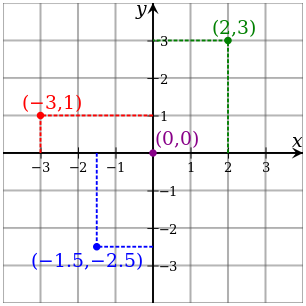
\includegraphics[width=1\textwidth]{figures/cau100.PNG}}
	\caption{penentuan garis/titik dalam diagram kartesius}
	\label{cau100}
	\end{figure}

Perhatikan diagram Cartesius pada gambar di atas. Warna ungu (violet) merupakan pusat koordinat yaitu titik (0,0) yang artinya sumbu x dan y bernilai nol. Untuk warna hijau, pada sumbu x bernilai 2 dan sumbu y bernilai 3 maka koordinat dalam bidang cartesius ditulis (2,3). Untuk warna merah, pada sumbu x bernilai  – 3 dan sumbu y bernilai 1 maka koordinat dalam bidang cartesius ditulis (– 3, 1). Sedangkan untuk warna biru, pada sumbu x bernilai  – 3 dan sumbu y bernilai 1 maka koordinat dalam bidang cartesius ditulis (–1.5 , –2.5).

Menurut wikipedia, istilah Cartesius digunakan untuk mengenang ahli matematika sekaligus filsuf dari Perancis bernama Descartes. Beliau memiliki peranan yang sangat besar dalam menggabungkan aljabar dan geometri (Cartesius adalah latinisasi untuk Descartes). Hasil kerjanya sangat berpengaruh dalam perkembangan geometri analitik, kalkulus, dan kartografi.




\chapter[Benua]
{Pengantar\\ benua}
% Kelompok Sejarah Benua dan Koordinat
% Agien Farhan S (1154012)
% Berlin Mitra Putra A (1154061)
% Indra Riksa Herlambang (1154051)
% Indra Saryoni Simanjuntak (1154115)
% Kindi Herdiansyah (1154048)

\section{Sejarah Benua}

\subsection{Benua pertama}
Mantel konveksi, proses yang mendorong lempeng tektonik adalah hasil dari aliran panas dari dalam bumi ke permukaan bumi \cite{suryasejarah}.Termasuk juga penciptaan lempeng tektonik di pegunungan bawah laut. Lempeng ini dihancurkan oleh subduksi di zona subduksi. Pada awal eon Arkean \ref{PetaAmerikaUtara} (sekitar 3 miliar tahun yang lalu) mantel itu jauh lebih panas mungkin sekitar 1600° C, sehingga proses konveksi terjadi lebih cepat.

Kerak bumi mulai terbentuk saat permukaan bumi mulai memadat, menghilangkan bekas-bekas pergeseran lempeng tektonik Hadean. Namun, diperkirakan kerak bumi memiliki komposisi Basalt seperti Kerak samudera .Potongan kerak benua besar yang pertama, muncul saat akhir masa Hadean, sekitar 4 miliar tahun yang lalu.  Kraton adalah bagian kecil yang tersisa dari benua pertama. Potongan-potongan yang terjadi pada akhir Hadean sampai awal Arkean membentuk inti lempengan yang tumbuh menjadi benua seperti sekarang.

Batuan tertua ditemukan di Laurentia, Kanada, yang berupa tonalit yang berumur sekitar 4 miliar tahun. Bebatuan ini menunjukkan jejak metamorfosis oleh suhu tinggi,  dan biji-bijian sedimen yang terkena erosi selama terbawa oleh air, yang menunjukkan terdapat sungai dan laut pada 4 miliar tahun yang lalu.

\begin{figure}[ht]
    \centerline{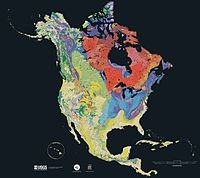
\includegraphics[width=1\textwidth]{figures/PetaAmerikaUtara.JPG}}
    \caption{Peta geologi Amerika Utara, kode warna menunjukan usia. Warna merah dan pink menunjukkan batuan dari masa eon Arkean.}
    \label{PetaAmerikaUtara}
    \end{figure}


\subsection{Benua raksasa pada masa Proterozoikum} 
Rekonstruksi pergerakan lempeng tektonik pada 250 juta tahun terakhir ( pada era Kenozoikum dan mesozoikum) dapat dilakukan dengan melihat kecocokan benua, anomali magnetik dasar laut, dan kutub paleomagnetik \cite{suryasejarah}. Para ahli tidak menemukan kerak samudera yang terbentuk sebelum waktu tersebut, sehingga rekonstruksi sebelum waktu tersebut sulit untuk dilakukan. Kutub paleomagnetik dilengkapi dengan bukti geologi seperti sabuk orogenik, yang menandai tepi lempeng kuno, dan distribusi flora dan fauna pada masa itu.

Sepanjang sejarah bumi, ada saat dimana benua bertabrakan dan membentuk benua raksasa, yang kemudian pecah menjadi benua baru. Sekitar 1000–830 juta tahun yang lalu, benua yang paling luas bersatu membentuk sebuah benua raksasa Rodinia. Sebelum Rodinia terbentuk, diperkirakan telah terbentuk terlebih dahulu Columbia atau Nuna pada awal sampai pertengahan masa Proterozoikum.

Setelah Rodinia pecah sekitar 800 juta tahun lalu, benua-benua tersebut kemungkinan telah membentuk benua raksasa lain yang berumur pendek yaitu , Pannotia \ref{BenuaRaksasaPannotia} pada 550 juta tahun lalu. Hipotetis benua raksasa mengacu pada Pannotia atau Vendia. Bukti yang memperkuat hipotesis tersebut adalah fase tabrakan benua yang diketahui sebagai orogeni Pan-Afrika, yang bergabung dengan benua Afrika , Amerika Selatan, Antartika dan Australia. Keberadaan Pannotia ditentukan oleh terjadinya retakan antara Gondwana (sebagian besar termasuk daratan di belahan bumi selatan, serta meliputi Semenanjung Arab dan anak benua India) dan Laurentia (kira-kira setara dengan Amerika Utara pada masa sekarang).Hal ini meyakinkan bahwa pada akhir masa eon Proterozoikum, sebagian besar benua bergabung dalam posisi di sekitar kutub selatan.

\begin{figure}[ht]
    \centerline{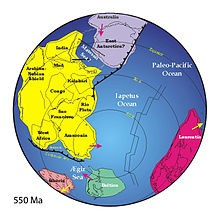
\includegraphics[width=1\textwidth]{figures/BenuaRaksasaPannotia.JPG}}
    \caption{Rekonstruksi benua raksasa Pannotia (warna kuning) pada 550 juta tahun lalu.}
    \label{BenuaRaksasaPannotia}
    \end{figure}


\subsection{Bukti Tersusunnya Benua Kuno}
Terdapat bukti dari para ahli yang digunakan untuk memperkirakan tersusunnya benua kuno.
Menurut Alfred Wegener(1880-1930), bahwa semua benua pernah bersatu kemudian berpecah menjadi sekarang ini dan benua yang bersatu itu dinamakan Pagaea (Benua Besar)\cite{hallam1975alfred}. Kemudian para ahli meneliti tentang benua dan membuat spekulasi-spekulasi teoritis yaitu melihat pada peta bahwa benua saling melengkapi dilihat dari garis pantai yang saling melengkapi seperti bagian puzzle. Kemudian meneliti fosil, bukti lain dari kehidupan lampau yaitu Mesosaurus. Mesosaurus adalah reptilia purba yang hanya hidup di air tawar dan ternyata hanya ada dua kawasan didunia yang memiliki fosil Mesosaurus ini yaitu Pantai Timur Amerika Selatan dan Pantai Barat Afrika. Kesimpulannya, fosil yang sama telah ditemukan di dalam batuan di kedua sisi lautan. Kemudian bukti korelasi batuan dan pegunungan telah ditemui di kedua belah sisi lautan. Yaitu meneliti banjaran pegunungan di Timur Laut Amerika Serikat dan banjaran pegunungan di Utara Eropa. Keduanya sangat sepadan atau keduanya tersusun daripada jenis batuan yang sama. Kemudian bukti data iklim masa lalu, terbukti pada Glacial Striations atau terdapat bentuk goresan pada batuan dan ini dapat dilihat dari hutan hujan tropika Amerika Selatan dan Afrika saat ini terdapat goresan glasier. Kesimpulannya adalah arang batu telah ditemukan di kawasan sejuk dan bukti glasier telah ditemui di kawasan panas berarti sebelumnya ada kemungkinan benua bersatu.

\section{Sejarah Koordinat}
Menurut ahli sejarah yang bernama Heroditus (450 M) menyatakan bahwa geometri berasal dari Mesir. Rane Discartes seorang matematikawan, yang lahir di sebuah Desa La Haye Prancis pada tahun 1596, adalah orang yang memiliki ketertarikan di bidang geometri. Rane Descrates telah menemukan sebuah metode untuk menyajikan sebuah titik sebagai bilangan berpasangan pada sebuah bidang datar. Bilangan-bilangan tersebut terletak pada dua garis yang saling tegak lurus antara satu dengan lainnya dan berpotongan di sebuah titik (0,0) dinamakan Origin , dan biasanya disimbolkan dengan huruf kapital O (0,0).
Bidang tersebut dinamakan bidang KOORDINAT atau yang lebih dikenal dengan bidang KARTESIUS.

\section{Sistem Koordinat}
Sistem koordinat dimaksudkan untuk memberikan peng-alamat-an terhadap setiap lokasi di permukaan bumi. Peng-alamatan dengan sistem kordinat didasarkan atas jarak timur-barat dan utara-selatan suatu tempat dari suatu titik pangkal tertentu. Jarak diukur dalam satuan derajat sudut yang dibentuk dari dari titik pangkal ke posisi tersebut melalui pusat bumi. Sedangkan titik pangkal ditetapkan berada di
perpotongan belahan utara-selatan bumi (garis katulistiwa) dengan garis yang membelah bumi timur- barat\cite{zuhdi2012sistem}.

Koordinat diambil untuk menjadi bilangan riil dalam matematika dasar, tetapi mungkin bilangan kompleks atau elemen-elemen dari sistem yang lebih abstrak. Penggunaan sistem koordinat memungkinkan masalah dalam angka untuk diterjemahkan ke dalam masalah-masalah tentang geometri dan juga sebaliknya.

\subsection{Sistem Koordinat Dua Dimensi}
\subsubsection{Sistem Koordinat Kartesius}
Koordinat Cartesius bukan merupakan satu-satunya jalan untuk menunjukkan kedudukan suatu titik pada bidang. Karena bentuk geometris di alam tidak selalu berupa kotak-kotak atau persegi panjang, namun adakalanya berbentuk lingkaran\cite{mufidah2015solusi}.Sistem koordinat Kartesius pada dua dimensi umumnya didefinisikan dengan dua buah sumbu yang saling tegak lurus antara satu dengan yang lainnya, yang keduanya terletak pada satu bidang (bidang xy). Sumbu horizontal(x), dan sumbu vertikal(y). Lalu, pada sistem koordinat tiga dimensi, ditambahkan sumbu yang lain yang sering diberi label z. Sumbu-sumbu tersebut ortogonal antar satu dengan yang lainnya. Titik pertemuan antara kedua sumbu, titik asal, pada umumnya diberi label 0. Setiap sumbu juga memiliki besaran panjang unit, dan setiap panjang tersebut diberi tanda dan membentuk semacam grid. Untuk mendeskripsikan suatu titik tertentu pada sistem koordinat dua dimensi, nilai absis(x), lalu diikuti dengan nilai ordinat(y). Dengan demikian, format yang dipakai selalu (x dan y) dan urutannya tidak dibalik-balik.

Gambar \ref{koordinat} Tanda panah yang ada pada sumbu berarti panjang sumbunya tak terhingga pada arah panah tersebut.

\begin{figure}[ht]
    \centerline{\includegraphics[width=1\textwidth]{figures/koordinat.JPG}}
    \caption{Keempat kuadran sistem koordinat Kartesius}
    \label{koordinat}
    \end{figure}

Pilihan huruf-huruf didasari oleh konvensi, yaitu huruf-huruf yang dekat akhir(x dan y) yang digunakan untuk menandakan variabel dengan nilai yang tidak diketahui, sedangkan huruf-huruf yang lebih dekat awal digunakan untuk menandakan nilai yang diketahui. Karena kedua sumbu saling bertegak lurus satu sama lain, bidang xy terbagi menjadi empat bagian yang disebut dengan kuadran, yang pada Gambar 3 ditandai dengan angka I, II, III, dan IV. Menurut konvensi yang berlaku, keempat kuadran tersebut diurutkan mulai dari yang kanan atas (kuadran I), melingkar melawan arah jarum jam (lihat Gambar 3). Pada kuadran I, kedua koordinat (x,y) bernilai positif. Pada kuadran II, koordinat x bernilai negatif dan koordinat y bernilai positif. Pada kuadran III, kedua koordinat mempunyai nilai negatif, dan pada kuadran IV, koordinat x bernilai positif dan y bernilai negatif. (lihat gambar \ref{contoh} dibawah ini).

\begin{figure}[ht]
    \centerline{\includegraphics[width=1\textwidth]{figures/contoh.JPG}}
    \caption{Nilai x dan y pada Kuadran I,II,III,IV}
    \label{contoh}
    \end{figure}

\subsubsection{Sistem Koordinat Polar}
Pada sistem koordinat polar, sepasang koordinat polar suatu titik ditulis dengan (𝑟,𝜃)\cite{mufidah2015solusi}.Konsep dari sudut dan radius sudah diterapkan oleh orang-orang pada zaman dahulu se-abad sebelum masehi. Para astronom yunani dan astrologhipparcuhus (190-120 BCE) menemukan sebuah tabel dari fungsi dawai yang memberikan panjang dawai dari setiap sudut dan terdapat referensi dari penggunaan koordinat polar untuk mengetahui posisi bintang.

Sejak abad ke-8 yang lalu, astronom mengembangkan cara untuk mengira-ngira dan menghitung arah dari mekah, kaabah- beserta jaraknya-dari seluruh lokasi dari bumi. Penghitungan penting yaitu penggantian dari koordinat polar ekuatorial dari mekkah kedalam bentuk koordinat polar hampir sama pada sistem yang merupakan pusat dari lingkaran besar melewati daerah yang dilewati dan kutub bumi, serta sudut polar yaitu garis yang melewati daerah tersebut dan titik antipodal.

Dalam Method of fluxion (tertulis 16711) Sir Isaac Newton menentukan hubungan antara koordinat polar, yang kemudian ia sebut dengan “ tujuh cara untuk spiral, dan sembilan sistem koordinat. 

\section{Geometri Koordinat}
 Pembelajaran subtajuk-subtajuk Geometri Koordinat, iaitu jarak antara dua titik, pembahagian tembereng garis, luas poligon, persamaan garis lurus, garis lurus selari dan garis lurus serenjang, persamaan lokus yang melibatkan jarak antara dua titik dan menentukan hubungan antara pencapaian responden dalam topik pelajaran\cite{shong2013analisis}.
 
 \subsection{Sketsa Grafik Garis}
 Sketsa grafik garis merupakan salah satu materi yang membahas mengenai penggambaran grafik garis lurus pada bidang kartesius berdasarkan persamaan yang diberikan. Materi ini mirip dengan metode penggambaran garis yang ada atau diajarkan pada aljabar. Maka jika sudah menguasai materi aljabar, sketsa grafik garis bukan masalah untuk dipelajari. Dalam menggambar grafik garis lurus, pertama harus melakukan pencarian pada nilai x dan y pada bidang kartesius dari persamaan yang sudah ada. Setelah nilai x dan y pada bidang kartesius telah di-temukan tentu bisa menentukan titiknya dan langsung menggambar garis tersebut.
 
 \subsection{Persamaan Garis Lurus}
 Persamaan garis lurus dapat di-definisikan sebagai perbandingan selisih nilai x dan y yang sudah melangkahi 2 titik pada garis. 
 Persamaan garis lurus terdapat satu komponen Gradien yaitu kecenderungan sebuah garis, gradien biasa dilambangkan dengan huruf m.
 Dalam materi persamaan garis lurus terdapat materi pokok seperti menentukan \"gradien" garis lurus, \"kedudukan" garis lurus,
 \"persamaan" garis melalui satu titik merupakan gradien, dan \"persamaan" garis melalui dua titik.
 
 \subsection{Pesamaan Lingkaran}
 Persamaan lingkaran adalah persamaan titik koordinat yang membentuk sebuah lingkaran pada bidang kartesius. Pada konsep ini jari lingkaran yang telah terbentuk adalah jarak dari himpunan titik koordinat ke titik pusat atau sebaliknya.Pada persamaan lingkaran yang dapat dipelajari seperti lingkaran yang memiliki pusat (0,0), lingkaran yang memiliki pusat (a,b).
 
 \subsection{Program Linear}
 Program linear adalah metode matematika yang digunakan untuk menyelesaikan soal-soal yang memiliki batas persamaan linear. Secara umum program linear terbagi atas 2 bagian yaitu fungsi kendala dan fungsi objektif. Penyelesaian program linear model matematika adalah suatu metode penerjemahan permasalahan ke dalam bentuk matematika, sehingga soal tersebut bisa diselesaikan secara matematis.
 
 \subsection{Pembelajaran Geometri Koordinat}
 Geometri Koordinat merupakan materi yang memberika pengujian ketrampilan dalam geometri dan aljabar.
 Jika sudah menguasai materi geometri dan aljabar maka bisa dinyatakan geometri koordinat tidak lagi membuat sulit untuk dipelajari.


\chapter[Sejarah Bumi]
{Pengantar\\ Sejarah Bumi}
% Nama Kelompok : Kelompok 4
% Akbar Pambudi Utomo (1154094) 
% Andi Nurfadilah Ali (1154041)
% Andi Wadi Afryandika (1154113)
% Hanna Theresia Siregar (1154009)
% Julham Ramadhana (1154069)
% Pebridayanti Hasibuan (1154118)

\section{Sejarah Bumi}
Bumi merupakan planet atau rumah kita dalam kedudukan di tata surya. peradaban kuno percaya bahwa bumi itu datar, dengan langit berputar-putar sekali sehari. secara umum yang diyakini bahwa kehidupan di Bumi dimulai di Bumi itu sendiri, beberapa waktu setelah terbentuknya planet antara 4000-5000 juta tahun yang lalu. namun ada yang berpendapat bahwa kehidupan diluar bumi itu ada, tetap kita tidak memiliki bukti pasti tentang kehidupan di tempat lain. yang perlu kita ketahui bumi berada pada galaksi bimasakti dimana terdapat matahari sebagai sistem bintang.
Dalam Geologi sendiri atau biasa disebut sebagai ilmu pengetahuan tentang Kebumian yang mempelajari segala sesuatu mengenai planet Bumi beserta isinya yang pernah ada. Dalam Geologi juga akan dibahas tentang sifat-sifat dan bahan- bahan yang membentuk bumi itu apa, serta struktur dan proses-proses yang bekerja baik didalam maupun dibagian teratas permukaan bumi, kedudukannya di Alam Semesta hingga sekarang. Geologi merupakan ilmu pengetahuan yang komplek, mempunyai pembahasan materi yang beraneka ragam namun juga merupakan ilmu pengetahuan yang enak dipelajari. Sebagai landasan prinsip untuk dapat mempelajari ilmu geologi adalah bahwasanya kita harus menganggap bumi ini sebagai suatu benda yang secara dinamis berubah sepanjang masa, setiap saat dan setiap detik. 
Pemikiran geologi modern dikenalkan oleh Huttonian revolution mengemukakan pemikiran-pemikirannya sebagai berikut:
1. Bahwasanya proeses-proses alam yang sekarang ini menyebabkan perubahan pada permukaan bumi, juga bekerja sepanjang umur dari bumi ini. 
2. Ia juga mengamati bahwa proses-proses tersebut yang walaupun bekerja sangat lambat, tetapi pada akhirnya mampu menyebabkan terjadinya perubahan-perubahan yang sangat besar pada bumi. 
3. Bahwa bumi ini sangat dinamis, yang berarti mengalami perubahan-perubahan yang terus-menerus mengikuti suatu pola daur (siklus) yang berulang-ulang.
Bumi sendiri berada di kawasan dimana terjadinya tumpang tindih antara litosfer (daratan) bagian padat dari bumi, hidrosfer (perairan), dan atmosfer (udara) yang menyelubungi bumi dengan zarah-zarah dan benda-benda yang mengisinya.
Dalam sejarah terbentuknya bumi sewaktu SMA kita pernah mempelajari teori-teori terbentuknya bumi dalam pelajaran geografi.\cite{wetherill1990formation}

\subsection{Teori-teori terbentuknya Bumi}
\subsubsection{1.Teori Kabut Kant-Laplace}
\begin{figure} [ht]
	\centerline{\includegraphics[width=1\textwidth]{figures/teorikabutnebula.JPG}}
	\caption{Gambar Teori Nebula}
	\label{teorikabutnebula}
	\end{figure}
	Pada Gambar berikut \ref{teorikabutnebula} adalah gambar dari Teori Kabut Nebula.
Teori ini dikenal dengan teori kabut (nebula) yang dikemukakan oleh Immanuel Kant (1755) dan Pierre de Laplace (1796). dalam teori ini dikemukakan bahwa di jagat raya terdapat gas yang kemudian berkumpul menjadi kabut(nebula). gaya tarik-menarik antargas ini membentuk kumpulan kabut yang sangat besar dan berputas semakin cepat sehingga materi kabut bagian khatulistiwa terlempar memisah dan memadat(karena pendinginan), bagian yang terlempar inilah yang kemudian menjadi sebuah planet dalam tatasurya. Bumi baru terus bertumbuh sampai suhu interiornya cukup panas untuk melelehkan logam siderofil. Dengan massa jenis yang lebih tinggi dari silikat, akhirnya logam ini tenggelam. Proses ini terjadi 10 juta tahun setelah Bumi mulai terbentuk, dan menghasilkan struktur Bumi yang berlapis-lapis dan mengakibatkan terbentuknya medan magnet. J. A. Jacobs merupakan orang pertama yang menunjukkan bahwa inti dalam—bagian dalam yang padat berbeda dari inti luar yang padat—membeku dan mengembang keluar inti luar yang cair dikarenakan bagian dalam bumi yang makin mendingin (sekitar 100° C per miliar tahun. Ekstrapolasi dari pengamatan ini memperkirakan bahwa inti terbentuk pada masa 2–4 miliar tahun yang lalu. Jika ini benar maka berarti bahwa inti bumi bukanlah fitur primordial yang berasal selama pembentukan planet.

\subsubsection{2.Teori Planetesimal}
\begin{figure} [ht]
	\centerline{\includegraphics[width=1\textwidth]{figures/teoriplanetesimal.JPG}}
	\caption{Gambar Teori Planetesimal}
	\label{teoriplanetesimal}
	\end{figure}
	Pada Gambar berikut \ref{teoriplanetesimal} adalah gambar dari Teori Planetesimal.
seabad kemudian sesudah teori kabut tersebut muncul teori Planetesimal yang dikemukakan oleh Chamberlin dan Moulton. Teori ini mengungkapkan bahwa pada mulanya telah terdapat Matahari asal. pada suatu ketika, matahari asal ini didedakti sebuah bintang besar yang menyebabkan terjadinya penarikan pada bagian matahari. Akibat tenaga tarik menarik tadi, terjadilah ledakan yang dasyat. Gas yang meledak ini keluar dari atmosfer matahari, kemudian mengembun dan membeku sebagai benda-benda yang padat(disebut planetesimal). Planetesimal ini dalam perkembangannya menjadi planet-planet, dan salah satunya planet bumi kita.

\subsubsection{3.Teori Pasang Surut Gas}
\begin{figure} [ht]
	\centerline{\includegraphics[width=1\textwidth]{figures/teoripasangsurut.JPG}}
	\caption{Gambar Pasang Surut}
	\label{teoripasangsurut}
	\end{figure}
	Pada Gambar berikut \ref{teoripasangsurut} adalah gambar dari Teori Pasang Surut.
Teori ini dikemukakan oleh Jeans dan Jeffreys, yakni bahwa sebuah bintang besar mendekati matahari dalam jarak pendek, sehingga menyebabkan terjadinya pasang surut pada tubuh matahari. dalam lidah yang panas ini terjadi perapatan gas-gas dan akhirnya kolom-kolom ini akan pecah, lalu berpisah menjadi benda-benda tersendiri yaitu planet-planet. bintang besar yang menyebabkan penarikan pad abagian-bagian tubuh matahari tadi melanjutkan perjalanan di jagat raya, sehingga lambat laun akan hilang pengaruhnya terhadapt planet-planet yang terbentuk tadi, lalu planet-planet itu akan mengelilingi matahari dan mengalami proses pendinginan, proses pendinginan berjalan lambat pada planet besar seperti yupiter dan saturnus, sedangkan planet kecil seperti bumi mengalami proses pendinginan yang relatif lebih cepat.

\subsubsection{4. Teori Bintang Kembar}
\begin{figure} [ht]
	\centerline{\includegraphics[width=1\textwidth]{figures/teoribintangkembar.JPG}}
	\caption{Gambar Teori Bintang Kembar}
	\label{teoribintangkembar}
	\end{figure}
	Pada Gambar berikut \ref{teoribintangkembar} adalah gambar dari Teori Bintang Kembar.
Teori ini dikemukakan oleh seorang ahli astronomi R. A. Lyttleton. Menurut teori ini, galaksi berasal dari kombinasi bintang kembar. Salah satu bintang meledak sehingga banyak materi yang terlempar. Karena bintang yang tidak meledak mempunyai gaya gravitasi yang masih kuat, maka sebaran pecahan ledakan bintang tersebut mengelilingi bintang yang tidak meledak. Bintang yang tidak meledak itu adalah matahari, sedangkan pecahan bintang yang lain itu adalah planet-planet yang mengelilinginya.

\subsubsection{5. Teori Dentuman Besar (Big Bang Teory)}
\begin{figure} [ht]
	\centerline{\includegraphics[width=1\textwidth]{figures/teoribigbang.JPG}}
	\caption{teoribigbang}
	\label{teoribigbang}
	\end{figure}
	Pada Gambar berikut \ref{teoribigbang} adalah gambar dari Teori Dentuman Besar(BigBang).
Pada Teori ini berdasarkan dari asumsi adanya massa yang sangat besar dan mempunyai massa jenis sangat besar. Adanya reaksi inti menyebabkan massa tersebut meledak hebat. Massa tersebut kemudian mengembang dengan sifat sangat cepat menjauhi pusat ledakan, karena danya gravitasi, maka bintang yang paling kuat gravitasinya akan menjadi pusatnya.
Dari berbagai teori, teori ini yang paling banyak didukung oleh para ilmuwan.

\section{Pendapat Tentang Sejarah Bumi}
Bumi terbentuk sekitar 4,54 miliar (4,54×109) tahun yang lalu melalui akresi dari nebula matahari. Pelepasan gas vulkanik diduga menciptakan atmosfer tua yang nyaris tidak beroksigen dan beracun bagi manusia dan sebagian besar makhluk hidup masa kini. Sebagian besar permukaan Bumi meleleh karena vulkanisme ekstrem dan sering bertabrakan dengan benda angkasa lain. Sebuah tabrakan besar diduga menyebabkan kemiringan sumbu Bumi dan menghasilkan Bulan. Seiring waktu, Bumi mendingin dan membentuk kerak padat dan memungkinkan cairan tercipta di permukaannya. Bentuk kehidupan pertama muncul antara 2,8 dan 2,5 miliar tahun yang lalu. Kehidupan fotosintesis muncul sekitar 2 miliar tahun yang lalu, nan memperkaya oksigen di atmosfer. Sebagian besar makhluk hidup masih berukuran kecil dan mikroskopis, sampai akhirnya makhluk hidup multiseluler kompleks mulai lahir sekitar 580 juta tahun yang lalu. Pada periode Kambrium, Bumi mengalami diversifikasi filum besar-besaran yang sangat cepat. Perubahan biologis dan geologis terus terjadi di planet ini sejak terbentuk. Organisme terus berevolusi, berubah menjadi bentuk baru atau punah seiring perubahan Bumi. Proses tektonik lempeng memainkan peran penting dalam pembentukan lautan dan benua di Bumi, termasuk kehidupan di dalamnya. Biosfer memiliki dampak besar terhadap atmosfer dan kondisi abiotik lainnya di planet ini, seperti pembentukan lapisan ozon, proliferasi oksigen, dan penciptaan tanah.Dalam sebuah artikel dari zuhdi2012sistem yang menyebutkan bahwa Bumi merupakan salah satu planet yang berada dalam tata surya yang diduga terbentuk dari pecahan-pecahan bintan pada jutaan tahun yang lalu, dan kemudian terperangkapa pada gravitasi matahari sehinggan akan selalu mengelilingi matahari. Menurut Hukum Newton kenapa planet dapat bertahan dalam pergerakan keliling atau biasa disebut revolusi dikarenakan planet melakukan gerak melingkar yang menimbulkan gaya sentifugal yang besarnya  dengan gaya gravitasi namun berlawanan arah. Gaya gravitasi ini sendiri akan berkurang sesuai dengan semakin jauhnya jarak planet dari matahari, sedangkan gaya sentrifugal  akan tergantung pada kecepatan gerak melingkar planet. Semakin cepat gerakan tersebut maka akan semakin besar daya sentifugal. Bila secara kebetulan kedua gaya ini memiliki kecepatan yang sama besar, maka planet akan terjebak mengelilingi matahari. Pada saat tata surya terbentuk diperkirakan terdapat jutaan planet. Akan tetapi sebagian terjatuh ke matahari atau terlempar lepas dari pengaruh matahari. Selain berkeliling, planet juga akan bergerak memutari pororsnya (rotasi). Gerak rotasi ini sendiri berlangsung dalan waktu lama sehingga membuat planet berbentuk seperti bola. Pada masa lalu, planet planet bukanlah sebuah benda padat, melainkan berupa magma atau berupa cairan batu. Bagian padat pada planet terbentuk selama proses pendinginan dan terjadi pada bagian kulit terluar dari planet tersebut. Bentuk Bumi sendiri yang dikatakan berbentuk bola tidakalah sempurna. Gerak Rotasi telah mengubah bentuk bumi menjadi agak cepat terhadap kedua kutubnya.\cite{zuhdi2012sistem}


Sejarah pembentukan Bumi yang dipelajari dalam materi pelajaran Geografi cenderung memiliki sifat abstrak yang akan lebih mudah dimengerti, jika memakai media yang cocok. Salah satu Inovasi pembelajaran yang tepat untuk dilakukan adalah menggunakan kartu indeks dan media film. Media seperti kartu indeks yang dipergunakan sebaga salah satu upaya yang memudahkan peserta didik agar mengingat konsep-konsep materi yang sedang dipelajari sedangkan media film sendiri merupakan media visual yang akan menjelaskan dengan lebih konkrit tentang fenomena bumi. Dalam sebuah artikel dari @article{widiyati2011meningkatkan menyebutkan bahwa Pmebentukan Bumi dengan kategori Continental Drift Theory atau biasa disebut dengan teori pengapungan benua yang dikemukan oleh Alfred Wegener pada tahun 1912 mengemukakan bahwa sampai sekitar 255 juta tahun lalu, di bumi baru ada satu benua dan samudera yang sangat luas. Benua raksasa ini sendiri dinamakan pangea, sedangkan kawasan samudera yang mengapitnya itu mengalami retakan-retakan dan pecah. Sekitar 135 juta tahun lalu, benua raksasa tersebut pecah menjadi dua, yaitu pecahan benua di sebelah utara yang dinamakan Lauransia dan dibagian selatan dinamakan gondwana.
\cite{widiyati2011meningkatkan}




\chapter[Garis Khatulistiwa]
{Pengantar\\ Garis Khatulistiwa}
   
								   
								   
												           Sejarah Garis Khatulistiwa Dan Prime Meridien
%Kelompok 4
% Eka Pratama Putra (1154023)
% Deni Braja Astrajingga (1154066)
% Luqman Nurfajri (1154054)
% Shinta Amelia (1154047)
% Yoshi Ricowandi Nababan (1154125)

														   
\section {Pendahuluan}

\subsection{pengertian garis khatulistiwa}	

	Dalam sebuah artikel dari Muhammad Adieb yang menyebutkan bahwa garis khatulistiwa merupakan garis lintang dari 0 derajat sampai dengan 90 derajat 
di kutub bumi. Jadi, nilai lintang berkisar antara 0° sampai dengan 90°. Di sebelah selatan garis khatulistiwa disebut lintang selatan (LS) dengan 
tanda negatif (-) dan di sebelah utara garis khatulistiwa disebut lintang utara (LU) yang diberi tanda positif (+). \cite {adieb2014studi}.

\subsection{pengertian prime meridian}
	
	Dalam sebuah artikel dari Mohd Zuhdi yang menyebutkan bahwa Prime meridian atau meridian Greenwich adalah nilai koordinat garis bujur dimulai dari 
bujur 0 derajat yaitu di Greenwich, kemudian membesar ke arah timur dan barat sampai bertemu kembali di Garis batas internasional yaitu terletak 
di Selat Bering dengan nilai 180 derajat. \cite {zuhdi2012sistem}.

	Dalam sebuah artikel lain oleh Andi Sunyoto yang menyebutkan bahwa Prime meridian adalah sebuah garis virtual yang melewati sebuah kota 
bernama Greenwich di Inggris. \cite{sunyoto2009api}.

\section {Isi}

\subsection{sistem koordinat bumi}
	
	Menurut sebuah artikel dari Mohd Zuhdi yang menyebutkan bahwa dalam sebuah artikel dari Mohd Zuhdi yang menyebutkan bahwa sistem koordinat dimaksudkan 
untuk memberikan pengalamatan terhadap setiap lokasi di permukaan bumi. pengalamatan dengan sistem koordinat didasarkan atas jarak timur sampai dengan barat 
dan utara sampai dengan selatan suatu tempat dari suatu titik pangkal tertentu. jarak diukur dalam satuan derajat dengan sudut yang dibentuk dari titik 
pangkal ditetapkan yang berada di perpotongan belahan utara sampai dengan selatan bumi (garis khatulistiwa) dengan garis yang membelah bumi bagian timur sampai 
dengan barat melewati kota GreenWhich di Inggris.

	
\begin{figure}[ht]
\centerline{\includegraphics[width=1\textwidth]{figures/garis_lintang_dan_bujur.PNG}}
\caption{menjelaskan tentang sudut lintang dan bujur pada bumi.}
\label{garis_lintang_dan_bujur}
\end{figure}

Pada gambar \ref{garis_lintang_dan_bujur} menjelaskan tentang sudut lintang dan bujur pada bumi.

	Posisi suatu tempat di alamatkan dengan nilai koordinat garis bujur (longitude) dan lintang (latitude) yang melalui tempat itu. Garis bujur (longitude), 
biasanya juga disebut garis meridian, yaitu merupakan garis lurus yang menyambungkan dari kutub utara sampai selatan bumi. Nilai koordinat garis bujur ini dimulai dari
bujur 0 derajat yaitu di Greenwich, kemudian membesar ke arah timur dan barat sampai bertemu kembali di Garis batas internasional yaitu terletak 
di Selat Bering dengan nilai 180 derajat. Garis bujur 0 derajat sering disebut prime meridien atau meridian Greenwich. Garis bujur ke arah barat diberi 
nilai negatif dan disebut bujur barat (west longitude) serta disingkat BB. Sedangkan garis bujur yang ke arah timur diberi nilai positif 
dan disebut bujur timur (east longitude) disingkat BT. Nilai koordinatnya didasarkan atas besarnya sudut yang terbentuk dari bujur 0 ke garis bujur tersebut
 melalui pusat bumi.

	Adapun nilai koordinat lintang dimulai dari garis lingkaran khatulistiwa yang diberi nilai 0 derajat. Selanjutnya garis-garis lintang yang lain berupa 
lingkaran-lingkaran paralel (sejajar) khatulistiwa berada di sebelah utara dan selatan khatulistiwa. Lingkaran paralel di selatan disebut garis lintang selatan (LS)
dan diberi nilai negatif, sedangkan lingkaran paralel di utara  diberi  nilai positif dan disebut garis lintang utara (LU). Nilai maksimum koordinat 
garis lintang adalah 90 derajat yaitu terletak di kutub-kutub bumi.

	Lingkaran paralel yang merupakan representasi garis lintang ini semakin mengecil ukurannya dengan semakin jauh dari khatulistiwa. Sehingga jarak 1 derajat 
timur sampai barat hanya beberapa meter saja. Itu sebabnya grid yang dibuat dari garis lintang dan garis bujur, tampaak berupa bujur sangkar di khaatulistiwa 
dan berubah menjadi persegi panjang di daerah dekat kutub. \cite {zuhdi2012sistem}.

\subsection (pemanfaatan prime meridian)

	Meridian Utama atau Prime Meridien digunakan untuk menentukan waktu di dunia, metode penentuannya akan dijelaskan sebagai berikut

\subsubsection(sistem penentuan waktu dunia)
	
	Menurut sebuah artikel dari Misbah Khusurur dan Jaenal Arifin yang menyebutkan bahwa Waktu Universal (bahasa Inggris Universal Time, disingkat UT)
adalah satu ukuran waktu yang didasari oleh rotasi bumi. Satuan ini adalah model perhitungan modern dari GMT (Greenwich Mean Time), yaitu mean waktu matahari 
di meridian di Greenwich, Inggris, yang biasanya dianggap sebagai bujur geografis 0 derajat GMT ini merupakan waktu 4 pertengahan yang yang di dasari oleh 
garis bujur yang melalui Greenwhich (BB/BT 0°) dan digunakan sebagai standar waktu Dunia Internasional.
	
	Sebelum diperkenalkannya standar waktu, setiap kota menyetel waktunya sesuai dengan posisi matahari di tempat masing-masing. Sistem ini bekerja 
dengan baik sampai diperkenalkannya transportasi kereta api untuk berpergian dengan cepat. akan tetapi, memerlukan seseorang untuk terus-menerus mencocokan 
jamnya dengan waktu lokal yang berbeda-beda dari satu kota ke kota lain. Standar waktu, dimana semua jam di dalam satu daerah menggunakan waktu yang sama, 
dibuat untuk memecahkan masalah perbedaan waktu seperti dalam perjalanan kereta api di atas.

	Standar waktu ini membagi bumi kedalam beberapa bagian ”zona waktu”, masing-masing bagiannya mencakupi dengan paling sedikit 15 derajat. Semua jam di dalam
zona waktu ini disetel sama dengan jam lainnya, tapi berbeda sebanyak satu jam dari jam-jam di zona waktu yang bertetanggaan. 
Waktu lokal di Royal Greenwich Observatory di Greenwich, Inggris, dipilih sebagai standard waktu dunia setelah terjadi 
Konferensi Meridian Internasional tahun 1884, yang memicu penyebaran pemakaian Greenwich Mean Time untuk menyetel jam di dalam suatu daerah. 
Lokasi ini dipilih sampai tahun 1884, 66 % dari semua peta dan tabel menggunakan greenwhich sebagai meridian utama (prime meridian).

\begin{figure}[ht]
\centerline{\includegraphics[width=1\textwidth]{figures/pembagian_waktu_dunia.PNG}}
\caption{menjelaskan tentang zona waktu pada tiap belahan dunia.}
\label{pembagian_waktu_dunia}
\end{figure}

Pada gambar \ref{pembagian_waktu_dunia} menjelaskan tentang zona waktu pada tiap belahan dunia.

	Perbedaan GMT dengan waktu pertengahan setempat di luar Greenwich adalah tergantung besar kecilnya Garis Bujur (BB/BT) dan dapat dirumuskan 
sebagai berikut:
\begin{equation}
WP x = GMT + BT, 
\end {equation}
atau 
\begin{equation}
WP x = GMT – BB
\end {equation}

\begin{equation}
GMT = WP x - BT, 
atau
\end{equation}
\begin{equation}
GMT = WP x + BB
\end{equation}
Contohnya sebagai berikut:

\begin {enumerate}
\item
Diketahui BT Semarang = 110° 26’
Pada saat GMT menunjukkan pukul 11.30, 
\begin{equation}
WP x = WP Semarang = 11.30 + 110° 26’
= 11.30 + 7 j 21m 44dt
= 18 j 51 m 44 dt
\end{equation}

\item
Diketahui BT Semarang = 100° 26’
Pada saat WP Semarang menunjukkan pukul 19.54,
\begin{equation}
GMT = 19.54 - 100° 26’
    = 19.54 - 8 j 24m 0dt
    = 11.30
\end{equation}
\end {enumerate}

\cite {khusurur2016mengenal}

\subsection {Dampak wilayah yang dilalui oleh garis khatulistiwa}

	Menurut sebuah artikel dari Yanti, Ari Hepi and Dhewiyanty, Varla and Setyawati, Tri Rima yang menyebutkan bahwa daerah yang dilalui garis khatulistiwa 
memiliki iklim tropis dengan suhu udara cukup tinggi dan kelembaban yang tinggi. Contoh daerah yang dilalui garis khatulistiwa yaitu Kalimantan Barat
suhu udara di Kalimantan Barat pada tahun 2013 berkisar antara 21,5oC-34,3oC (BPS Kalbar, 2014). \cite {yanti2015prevalensi}

	Masih ada lagi beberapa negara yang dilalui oleh garis khatulistiwa yang terdapat pada gambar \ref{tabel_negara_yang_dilalui_garis_khatulistiwa}

\begin{figure}[ht]
\centerline{\includegraphics[width=1\textwidth]{figures/tabel_negara_yang_dilalui_garis_khatulistiwa.PNG}}
\caption{list negara yang dilalui garis khatulistiwa.}
\label{tabel_negara_yang_dilalui_garis_khatulistiwa}
\end{figure}

	Pada gambar \ref{tabel_negara_yang_dilalui_garis_khatulistiwa} disebutkan negara - negara yang dilalui oleh garis khatulistiwa yaitu Sao Tome dan Pricipe 
yang terdapat pada benua Afrika, Gabon yang terdapat di benua Afrika, Republik Kongo yang terdapat di benua Afrika, Republik Demokratif Kongo yang terdapat 
di benua Afrika, Uganda yang terdapat di benua Afrika, Kenya yang terdapat di benua Afrika, Somalia yang terdapat di benua Afrika, Maladewa yang terdapat 
di benua Asia, Indonesia yang terdapat di benua Asia, Negara Kiribati , Ekuador yang terdapat di benua Amerika Selatan, Kolombia 
yang terdapat di benua Amerika Selatan, dan Brasil yang terdapat di benua Amerika Selatan
	
	untuk lebih detailnya terdapat pada gambar \ref{Peta_Dunia_Negara_Khatulistiwa}
	
\begin{figure}[ht]
\centerline{\includegraphics[width=1\textwidth]{figures/Peta_Dunia_Negara_Khatulistiwa.JPG}}
\caption{wilayah di dunia yang dilewati garis khatulistiwa.}
\label{Peta_Dunia_Negara_Khatulistiwa}
\end{figure}

\subsubsection {Peristiwa Equinox}

	Dalam sebuah artikel dari Mutoha Arkanudin yang menyebutkan bahwa selama setahun Matahari berubah posisi dari Utara ke Selatan dan sebaliknya. 
Posisi tersebut sering disebut sebagai Gerak Musim Matahari. Equinox adalah saat dimana posisi matahari berada tepat di Ekuator atau garis katulistiwa. 
Ini adalah bagian dari siklus tahunan pergerakan harian semu matahari saat terbit, melintas dan terbenam yang disebabkan oleh kemiringan sumbu bumi
terhadap bidang orbitnya yaitu sebesar 66.56 derajat. Selama setahun terjadi dua kali Equinox yaitu Maret Equinox yang terjadi setiap tanggal 21 Maret dan September
Ekuinox yang terjadi setiap tanggal 23 September. 

	Saat terjadi peristiwa Equinox posisi Matahari terbenam akan tepat berada di titik Barat sehingga dengan menambah sudut kemiringan arah kiblat 
terhadap titik Barat maka arah kiblat yang sesungguhnya kan kita dapatkan. 

	Selain Equinox matahari juga akan berada di titik paling Utara pada 21 Juni dan berada di titik paling Selatan pada 22 Desember yang dikenal dengan 
istilah Solstice. Pada saat Juni Solstice, Matahari akan terbenam tepat di sudut serong terhadap arah Barat sebesar 23,5 derajat ke arah Utara
sehingga untuk menuju ke arah kiblat yang tepat dapat tinggal menambahkan kekurangan penyerongan angka arah kiblat yang didapatkan dari hasil perhitungan 
menggunakan rumus segitiga bola. Sedangakan pada saat Desember Solstice matahari terbenam di Selatan titik Baratsebesar 23,5 derajat.\cite {arkanudin2008teknik}.

\section {Penutup}

\subsection{Kesimpulan}
	
	Garis khatulistiwa merupakan garis lintang dari 0 derajat sampai dengan 90 derajat di kutub bumi. Prime meridian atau meridian Greenwich adalah 
nilai koordinat garis bujur dimulai dari bujur 0 derajat yaitu di Greenwich, kemudian membesar ke arah timur dan barat sampai bertemu kembali di Garis batas 
internasional yaitu terletak di Selat Bering dengan nilai 180 derajat. Sistem koordinat dimaksudkan untuk memberikan pengalamatan terhadap setiap lokasi 
di permukaan bumi. Meridian Utama atau Prime Meridien digunakan untuk menentukan waktu di dunia, metode penentuan mengikuti Waktu Universal (bahasa 
Inggris Universal Time, disingkat UT) adalah satu ukuran waktu yang didasari oleh rotasi bumi. daerah yang dilalui garis khatulistiwa memiliki iklim tropis 
dengan suhu udara cukup tinggi dan kelembaban yang tinggi.

\subsection{Saran}

	Dalam artikel ini belum ada penjelasan mengenai sejarah garis khatulistiwa dan prime meridien, maka diharapkan untuk  kedepannya dilengkapi dengan 
informasi mengenai sejarah dari garis khatulistiwa dan prime meridien.	


\chapter[Kordinat Indonesia]
{Pengantar\\ Kordinat Indonesia}
% Nama kelompok : 3
% Kelas : D4 Teknik Informatika 3C
% 1. Kezia Tirza Naramessakh (1154093)
% 2. Mariani Rospilinda Siki (1154107)
% 3. Doli Jonviter Nt Simbolon (1154016)
% 4. Benedictus Simantupang (1154116)
% 5. Dimas Mathovani 


\section{Koordinat Lintang Utara, Lintang Selatan, Bujur Timur, Bujur Barat}
Koordinat digunakan untuk menunjukkan suatu titik di Bumi berdasarkan garis lintang dan garis bujur. Koordinat dibagi menjadi dua bagian irisan yaitu irisan melintang yang disebut dengan garis lintang mulai dari khatulistiwa, membesar ke arah kutub(utara maupun selatan) sedangkan yang lain membuju r mulai dari garis Greenwhich membesar ke arah barat dan timur. Satuan skala koordinat dibagi dalam derajat lintang 0* sampai 90* dan bujur 0* sampai 180*. Koordinat ini ditulis dalam satuan derajat, menit, dan detik, misalnya 110*35'32", dan seterusnya. Untuk membagi dunia dalam wilayah utara dan selatan, maka ditentukan sebuah garis yang tepat berada di tengah, yaitu garis Equator / Khatulistiwa. Untuk membagi wilayah timur dan barat, maka ditentukan sebuah garis Prime meridian yang terletak di kota Greenwich (Inggris), dan perpotongannya bertemu di wilayah laut pasific, yakni memotong kepulauan Fiji.
Koordinat pada gambar \ref{Koordinat} di jelaskan garis Lintang dan Bujur
\begin{figure}[ht]
	\centerline{\includegraphics[width=1\textwidth]{figures/Koordinat.JPG}}
	\caption{Koordinat Lintang dan Bujur}
	\label{Koordinat}
	\end{figure}

\subsection{Sistem Koordinat}
Dalam artikel Zuhdi menjelaskan Koordinat dimaksudkan untuk memberikan pengalamatan terhadap setiap lokasi di permukaan bumi. Pengalamatan dengan sistem koordinat didasarkan atas jarak timur-barat dan utara-selatan suatu tempat dari suatu titik pangkal tertentu. Jarak diukur dalam satuan derajat sudut yang dibentuk dari titik pangkal ke posisi tersebut melalui pusat bumi. Sedangkan titik pangkal ditetapkan berada di perpotongan belahan utara-selatan bumi (garis khatulistiwa) dengan garis yang membelah bumi timur-barat melalui kota GreenWhich di Inggris. 
Untuk lebih jelas tentang bentuk titik koordinat lihat pada gambar \ref{sistemkoordinat} dibawah ini :
\begin{figure}[ht]
	\centerline{\includegraphics[width=1\textwidth]{figures/sistemkoordinat.JPG}}
	\caption{Bentuk titik Koordinat}
	\label{sistemkoordinat}
	\end{figure}

Baik garis lintang maupun garis bujur diukur dalam derjat dan dibagi lagi dalam menit dan detik. 1 derajat garis bujur diukur lapangan sama dengan 11,32 km. Satuan derajat bisa juga disebut jam sehingga setiap derajat terbagi menjaid 60 menit dan setiap menit terbagi menjadi 60 detik. Dalam penulisan letak astronomis contohnya 60 derajat 23' 15"S, maka dibaca sebagai 60 derajat 23 menit 15 detik lintang selatan. pada sistem pemetaan internasional huruf U sebagai lintang utara diganti dengan huruf N (north). Besar sudut dalam sistem koordinat geografik dapat dinyatakan dalam dua cara, yaitu dengan satuan DMS(Degree Minute Second) atau satuan DD(Decimal Degree), dalam sistem satuan DMS, setiap derajat sudut dibagi menjadi 60 menit dan setiap menitnya dibagi lagi menjadi 60 detik. Penulisannya dinyatakan sebagai dd°mm'ss". Sedangkan pada sistem satuan setiap derajatnya dinyatakan dalam pecahan decimal (pecahan berkoma). Baik dalam DMS maupun DD, perlu diketahui berapa ketelitian suatu nilai koordinat. Karena di wilayah khatulistiwa jarak 1° sama dengan jarak 111321 meter. Maka perlu diperhatikan keselahan yang terjaddi jika kita mengabaikan suatu angka menit atau detik pada DMS atau suatu nilai digit dalam koordinat DD. Pada sistem DD, perlu diperhatikan jarak yang diwakili oleh setiap digit dibelakang koma. Perubahan satu satuan padaa digitt pertamma dii belakang koma mempunyai nilai jarak lebih dari 11 Km. Perubahan satu unit pada digit keduat dibelakang koma berarti 1,1 Km. Demikian seterusnya. Berarti jika kita misalnya hanya mentolerir kesalahan sampai 100 m, maka koordinat DD harus dibuat setidaknya sampai 4 digit di belakang koma. Kombinasi antara garis lintang dan garis bujur akan membentuk sutau koordinat lokasi di permukaan bumi dengan sumbu x sebagai garis lintang dan sumbu y sebagai garis bujur dalam koordinat kartesius. Pada Bujur/Longitude (X) merupakan garis yang perpindahannya secara vertical dan pada Lintang/Lattitude (Y) merupakan garis yang mempunyai perpindahan secara horizontal. \cite{zuhdi2012sistem}.

Lihat pada gambar \ref{lintangbujur} dibawah ini :
\begin{figure}[ht]
	\centerline{\includegraphics[width=1\textwidth]{figures/lintangbujur.JPG}}
	\caption{Titik Lintang dan Bujur}
	\label{lintangbujur}
	\end{figure}

\subsubsection{Garis Lintang}
Sebuah garis khayal yang digunakan untuk menentukan lokasi di Bumi terhadap garis khatulistiwa(utara atau selatan). Posisi lintang merupakan penghitungan sudut dari 0 derajat di khatulistiwa sampai ke +90 derajat di kutub utara dan -90 derajat di kutub selatan. Dalam bahasa indonesia lintang di sebelah utara khatulistiwa diberi nama Lintang Utara(LU), demikian pula lintang di sebelah selatan khatulistiwa diberi nama Lintang Selatan(LS). Lintang Utara dan Lintang Selatan menyatakan besarnya sudut antara posisi lintang dengan garis Khatulistiwa. Garis Khatulistiwa sendiri adalah lintang 0 derajat. 
Nilai koordinat lingtang dimulai dari garis lingkaran khatulistiwa yang diberi nilai 0 derajat. Selanjutnya garis lintang yang lain berupa lingkarang paralel (sejajar) katulistiwa berada disebelah utara dan selatan khatulistiwa. Lingkaran paralel di selatan disebut garis lintang selatan (LS) dan diberi nilai negatif, sedangkan lingkaran paralel diutara diberi nilai positif dan disebut garis lintang utara (LU). Nilai maksimum koordinat garis lintang adalah 90 derajat yaitu terletak di kutub-kutub bumi. 
Lingkaran paralel merupakan representasi garis lintang ini semakin mengecil ukurannya dengan semakin jauh dari katulistiwa. sehingga jarak 1 derajat timur-barat dari katulistiwa jauh lebih besar dari pada jarak 1 derajat timur-barat di tempat yang jauh dari katulistiwa. Di khtulistiwa 1 derajat timur-barat sama dengan 111.321 km, tapi di dekat kutub 1 derajat timur-barat hanya beberapa meter saja. itu sebabnya grid yang dibuat dari garis lintang dan garis bujur, tampak berupa sangkar dikatulistiwa dan berubah menjadi persegi didaerah kutub
lintang memiliki symbol phi dan menunjukkan sudut antara garis lurus dititik tertentu dengan bidang ekuator. Lintang ditentukan dalam angka derajat dimulai dari 0 derajat dan berakhir dengan 90 derajat. garis lintang ini membagi bumi menjadi belahan bumi utara dan selatan. garis ekuator atau khatulistiwa berada di lintang 0 derajat. Garis lintang biasa digunakan untuk melihat penyebaran iklim di bumi.
Latitude aau garis lintang adalah garis yang menentukan lokasi berada di sebelah utara atau selatan ekuator. garis lintang diukur mulai dari titik 0 derajat dari khatulistiwa sampai 90 derajat di kutub. Garis lintang digunakan untuk membatasi corak iklim di permukaan bumi, berikut ini merupakan pembagian iklim di bumi menurut batas garis lintang:
1. 23,5-23,5 LU/LS = iklim tropis
2. 23,5-40 LU/LS = iklim subtropis
3. 40 Lu-66,5 LU/LS = iklim sedang
4. 66,5-90 LU/LS = iklim kutub
Indonesia terletak antara 6 derajat Lintang Utara (LU) – 11 derajat Lintang Selatan (LS) dan diantara 95 derajat bujur timur – 141 derajat Bujur timur.
Adapun wilayah indonesia itu pada bagian paling utara yang ebrada di Pulau Weh di Nanggroe Aceh Darussalam yang terletak pada 6 derajat lintang utara, dan untuk daerah indonesia yang paling berada di selatan yaitu Pulau Roti di Nusa Tenggara Timur yang terletak pada 11 derajat lintang selatan. Kemudian mengacu pada letak lintangnya, di wilayah Indonesia berada pada 6 derajat lintang utara – 11 derajat lintang selatan, hal tersebut disebabkan indonesia mempunyai iklim tropis dengan beberapa ciri-ciri yaitu mempunyai hutan hujan tropis yang begitu luas dan mempunyai nilai ekonomis yang sangat tinggi, mendapatkan sinar matahari yang lama setiap sepanjang tahun, mempunyai curah hujan yang tinggi dan memiliki banyak penguapan sehingga akan meningkatkan kelembaban udara.
Pada gambar \ref{lintang} dijelaskan titik koordinat Lintang pada sumbuh Y :
\begin{figure}[ht]
	\centerline{\includegraphics[width=1\textwidth]{figures/lintang.JPG}}
	\caption{Titik koordinat Lintang pada sumbuh Y}
	\label{lintang}
	\end{figure}

\subsubsection{Garis Bujur}
Menggambarkan lokasi sebuah tempat di timur atau barat Bumi dari sebuah garis utara-selatan yang disebut Meridian Utama. Longitude diberikan berdasarkan pengukuran sudut yang berkisar dari 0 derajat Meridian Utama ke +180 derajat arah timur dan -180 derajat arah barat. Tidak seperti lintang yang memiliki ekuator sebagai posisi awal alami, tidak ada posisi awal alami untuk bujur. Bujur di sebelah barat Meridian diberi nama Bujur Barat(BB), demikian pula bujur di sebelah timur Meridian diberi nama Bujur Timur(BT).
Nilai koordinat garis bujur dimulai dari bujur 0 derajat yaitu Greenwhich, kemudian memebersasr ke arah timur dan barat sampai bertemu kembali di garis batas tanggal internasional yaitu terletak di selat bering dnegan nilai 180 derajat. garis bujur 0 derajat disebut prime meridian atau meridian greenwhich. garsi bujur ke arah barat diberi nilai negatif dan disebut bujur barat (west longitude) serta disingkan BB. sedangkan garis bujur yang ke arah timur diberi nilai positif dan disebut bujur timur (east longitude) disingkat BT. nilai koordinatnya didasarkan atas besarnya sudut yang terbentuk dari bujur 0 ke garis bujur tersebut melalui pusat bumi.
Longitude atau garis bujur memiliki symbol lamda. garis bujur ini merupakan garis yang menunjukkan bagian barat dan timur dilihat dari titik pangkal yaitu di greenwich meridian. garis bujur emiliki batas maksimum yaiu 180 derajat ke arah timur dar GMT dan 180 derajat ke arah barat dari GMT. keduanya bertemu di garis internasional date line disekitar pasifik.
longitude atau garis bujur digunakan untuk menentukan lokasi diwilayah barat atau timur dari garis utara selatan yang sering disebut juga garis meridian. garis bujur digunakan untuk menentukan waktu dan tanggal.
Titik di barat bujur 0° dinamakan Bujur Barat sedangkan titik di timur 0° dinamakan Bujur Timur. Kombinasi garis lintang dan garis bujur ini berguna untuk menentukan suatu lokasi di permukaan bumi. Garis Lintang menandakan sumbu y dan garus bujur menandakan sumbu x dalam sistem koordinat cartesian. Sebagi contoh kota Sabang di pulau We berada pada koordinat 6oLU 95o BT, dan kota Merauke di Papua memiliki koordinat 11oLS dan 141oBT.
Indonesia berada pada 95 derajat bujur timur – 141 derajat bujur timur menyebabkan Indonesia mempunyai tiga waktu dan pada setiap waktu memiliki daerah tersendiri, sehingga Indonesia memiliki beberapa pembagian waktu yaitu Waktu Indonesia bagian timur atau WIT mencakup Papua, kepulauan Maluku dan pulau-pulau kecil disekitarnya. Untuk waktu indonesia bagian  timur mempunyai selisih waktu sebanyak 9 jam lebih awal dari Greenwich Mean time atau GMT. Kemudian untuk Waktu Indonesia bagian tengah atau WITA mencakup Nusa tenggara, kalimantan selatan, Pulau Sulawesi, Bali dan pulau-pulau kecil yang ada disekitarnya. Untuk Indonesia bagian tengah mempunyai selisih waktu sebanyak 8 jam yang lebih awal dari Greenwich mean time (GMT). Kemudian, untuk daerah waktu Indonesia bagian barat atau WIB yang mencakup Madura, Jawa, kalimantan barat, kalimantan tengah, Sumatera dan pulau-pulau kecil yang ada disekitarnya. Adapun waktu indonesia bagian barat mempunyai selisih waktu sebanyak 7 jam yang lebih awal dari Greenwich mean time.
Pada gambar \ref{bujur} dijelaskan titik koordinat Lintang pada sumbuh X :
\begin{figure}[ht]
	\centerline{\includegraphics[width=1\textwidth]{figures/bujur.JPG}}
	\caption{Titik koordinat Bujur pada sumbuh X}
	\label{bujur}
	\end{figure}

\chapter[Kordinat Internasional]
{Pengantar\\ Kordinat Internasional}
% Nama Kelompok 2 : Latitude & Longitude
% Kelas : D4TI3C
% Adhika Dwi Cahya Putra (1154017)
% Haris Munandar Alwi (1154105)
% Muhammad Adam Nahdlotul Halimi (1154024)
% Tito Aryo Nugroho (1154074)
% Tomy Prawoto (1154121)

\section{latitude longitude}

\subsection{Latitude}
Latitude merupakan terjemahan bahasa inggris dari garis lintang. Garis lintang dapat disebut juga sebagai garis khatulistiwa (0 derajat), atau bisa disebut juga sebagai garis tengah bumi yang membagi antara belahan bumi bagian atas dan bumi bagian bawah.
Dalam sebuah buku karangan Maling \& Derek Hylton yang berjudul \"Coordinate System and Map Projections\" mengatakan bahwa garis lintang suatu titik dapat didefinisikan secara formal sebagai sudut yang diukur di tengah bumi di antara bidang equator dan jari jari yang ditarik ke titik. 
Pada garis lintang bagian utara bumi dilambangkan dengan tanda \verb|'+phi'| 
sedangkan garis lintang bagian selatan bumi dilambangkan dengan tanda \verb|'-phi'| 
\cite{maling2013coordinate}. 

	\begin{figure}[ht]
	\centerline{\includegraphics[width=1\textwidth]{figures/latitude.PNG}}
	\caption{Garis Lintang atau Latitude.}
	\label{latitude}
	\end{figure}
Pada gambar \ref{latitude} merupakan gambar latitude atau garis lintang yang membentang antara west(barat) sampai east(timur).
Garis lintang digunakan sebagai penanda dalam zona iklim di dunia. Dari +23 setengah derajat Lintang Utara sampai -23 setengah Lintang Selatan memiliki zona iklim tropis. Zona iklim tropis hanya memiliki dua musim, yaitu kemarau atau panas dan penghujan saja. Kemudian dari +23 setengah derajat Lintang utara sampai +66 setengah derajat Lintang utara memiliki zona iklim subtropis. Sama halnya bagian utara, bagian selatan yaitu -23 setengah derajat lintang selatan sampai -66 setengah derajat lintang selatan memiliki zona iklim subtropis. Daerah subtropis memiliki 4 musim, yaitu spring, summer, fall, dan winter. 

\subsection{Longitude}
Longitude merupakan terjemahan bahasa inggris dari garis bujur. Garis bujur biasa digunakan untuk menentukan waktu dan tanggal di dunia yang kita huni sekarang ini. Jika garis lintang atau latitude atau daerah khatulistiwa dianggap sebagai 0 derajat, maka garis bujur merupakan 0 derajat yang menghubungkan kutub utara dengan kutub selatan yang melawati kota Greenwich di Inggris. Garis bujur bagian barat kota Greenwich disebut sebagai Bujur Barat sedangkan garis bujur yang berada pada sebelah timur kota Greenwich disebut sebagai Bujur Timur. Inilah penyebab kenapa orang indonesia disebut sebagai orang timur.
	\begin{figure}[ht]
	\centerline{\includegraphics[width=1\textwidth]{figures/longitude.PNG}}
	\caption{Garis Bujur atau Longitude.}
	\label{longitude}
	\end{figure}
Pada gambar \ref{longitude} merupakan gambar longitude atau garis bujur yang menghubungkan kutub utara dengan kutub selatan. Garis ini melewati kota Greenwich di Inggris.
Garis bujur digunakan untuk pembagian zona waktu di dunia.

\section{LINTANG}

	Sudut lintang l
	Bayangkan Bumi adalah bola transparan (sebenarnya
	bentuknya agak oval; karena rotasi bumi, nya
	Khatulistiwa sedikit menonjol). Melalui Bumi yang transparan
	(gambar) kita bisa melihat bidang ekuatornya, dan bagian tengahnya
	titik adalah O, pusat bumi.
	Untuk menentukan garis lintang beberapa titik P di permukaan, tariklah
	radius OP ke titik itu. Maka sudut elevasi titik itu
	Di atas garis ekuator adalah garis lintang l - lintang utara jika utara
	dari garis khatulistiwa, lintang selatan (atau negatif) jika selatannya.
	Garis lintang. Di dunia bumi, garis lintang adalah lingkaran dengan ukuran yang berbeda. Itu
	terpanjang adalah khatulistiwa, yang garis lintangnya nol, sementara di kutub - di garis lintang
	90 ° utara dan 90 ° selatan (atau -90 °) lingkaran menyusut ke titik tertentu.

\section{GARIS BUJUR}
	Di dunia, garis bujur konstan ("meridian") meluas dari tiang ke kutub, seperti
	batas segmen pada jeruk kupas.
	Garis bujur atau "garis meridian"
	Setiap meridian harus melewati garis khatulistiwa. Karena ekuator adalah lingkaran, kita bisa
	bagilah itu - seperti lingkaran - ke dalam 360 derajat, dan bujur f dari sebuah titik adalah
	maka nilai yang ditandai dari divisi mana meridiannya memenuhi khatulistiwa.
	Apa nilai itu tergantung tentu saja dari mana kita mulai menghitung - di mana
	nol bujur adalah Untuk alasan historis, garis meridian melewati Astronomi Kerajaan yang lama
	Observatorium di Greenwich, Inggris, adalah yang dipilih sebagai nol bujur. Bertempat di Jl
	Tepi timur London, ibu kota Inggris, observatorium sekarang menjadi museum umum dan a
	band kuningan yang membentang di halamannya menandai "garis meridian utama". Wisatawan sering mendapatkan
	difoto saat mereka mengangkangnya - satu kaki di belahan bumi bagian timur, yang lainnya masuk belahan barat.
	Garis bujur juga disebut meridian, berasal dari bahasa Latin, dari meri, a
	variasi "medius" yang menunjukkan "tengah", dan diem, yang berarti "hari". Kata itu
	pernah berarti "siang", dan waktu sehari sebelum siang hari dikenal sebagai "ante meridian",
	sementara waktu setelah itu adalah "posting meridian." Singkatan hari ini a.m. dan p.m. datang
	Dari istilah ini, dan Matahari pada siang hari dikatakan "melewati meridian". Semua poin di
	garis bujur yang sama mengalami siang hari (dan jam lainnya) pada saat bersamaan dan
	oleh karena itu dikatakan sama "garis meridian", yang menjadi "meridian" untuk
	pendek.

\section{Waktu Lokal (LT) dan Zona Waktu}
	Garis bujur diukur dari nol sampai 180 ° BT dan 180 ° BB (atau -180 °), dan kedua 180-
	Gelombang longitudinal berbagi jalur yang sama, di tengah Samudera Pasifik.
	Saat Bumi berputar mengelilingi porosnya, kapanpun satu garis bujur - "siang hari
	meridian "- menghadap Matahari, dan pada saat itu, akan ada siang hari di mana-mana di atasnya
	jam Bumi telah mengalami rotasi penuh sehubungan dengan Matahari, dan meridian yang sama
	lagi wajah siang hari Jadi setiap jam Bumi berputar 360/24 = 15 derajat.
	Bila di lokasi Anda waktu 12 siang, 15 ° ke timur waktu adalah 1 p.m., karena itu adalah
	meridian yang dihadapi Matahari sejam yang lalu. Di sisi lain, 15 ° ke barat waktu adalah 11
	a.m., untuk satu jam lagi, meridian itu akan menghadapi Matahari dan mengalami siang hari.

\subsection{Glosarium}
	Khatulistiwa-Garis yang mengelilingi Bumi pada jarak yang sama dari Utara dan Selatan
	Polandia Koordinat geografis - Koordinat nilai yang diberikan sebagai garis lintang dan bujur.
	Lingkaran besar - Sebuah lingkaran terbentuk di permukaan bola oleh sebuah pesawat yang melewati
	pusat bola. Khatulistiwa, masing-masing meridian, dan satu sama lain keliling penuh
	Bumi membentuk lingkaran besar. Arus lingkaran besar menunjukkan jarak terpendek antara titik-titik di permukaan bumi.

	\subsubsection{Meridian}
	Lingkaran besar di permukaan Bumi, melewati kutub geografis
	dan beberapa titik ketiga di permukaan bumi. Semua poin pada meridian tertentu memiliki hal yang sama
	\subsubsection{Paralel}
	Lingkaran atau perkiraan lingkaran di permukaan Bumi, sejajar dengan
	Khatulistiwa dan titik penghubung dengan garis lintang yang sama.
	\subsubsection{Prime Meridian}
	Garis meridian bujur 0 derajat, digunakan sebagai asal untuk
	pengukuran bujur. Garis meridian Greenwich, Inggris, adalah internasional
	menerima meridian utama dalam banyak kasus.

\section{Konversi antara koordinat geografis dan cartesian koordinat}
	Asumsikan bahwa koordinat geografis dari suatu titik M adalah l dan f; asumsikan bahwa jari - jari
	Bumi adalah R. Masalahnya adalah penentuan koordinat kartesius M dalam a
	Sistem koordinat asal pusat bumi, dengan bidang horisontal xoy bidang
	Khatulistiwa, dengan sumbu x melewati meridian Greenwich, sumbu y secara langsung
	tegak lurus dengan sumbu x, dan akhirnya sumbu z melewati kutub.
	Tujuannya adalah untuk menemukan x, y dan z.

	Tunjukkan pada gambar sudut l dan f;
	Berapakah jarak OM?
	Hitung jarak OH menurut l.
	Berapakah nilai x dan y menurut l dan f;
	Berapakah nilai z?
	Asumsikan bahwa koordinat geografis dari suatu titik V
	adalah:
	garis lintang: 45 ° 41'47.59 '' N
	Bujur: 4 ° 52 '+ 49,98' 'E
	Apa koordinat kartesian V (dengan R = 1)
	Sebenarnya, titik ini persis sekolah kita!

\section{LINTANG/LATITUDE}

	Latitude adalah garis mendatar. Titik 0 adalah sudut ekuator tanda + menunjukan arah ke atas menuju kutub utara,
	sementara tanda minus di koordinat menuju ke kutub selatan. Bayangkan bila bumi hanyalah sebuah bola transparan 
	(sebenarnya bentuk bumi adalah oval; ini dikarenakan rotasi bumi itu sendiri, karena garis khatulistiwa sedikit 
	terlihat). Dengan bumi yang transparan, kita bisa lihat (gambar)
	\begin{figure}[ht]
	\centerline{\includegraphics[width=1\textwidth]{figures/Latitude.jpg}}
	\caption{gambar Latitude.}
	\label{Gambar Latitude}
	\end{figure}
	garis khatulistiwa bumi, dan garis tengahnya adalah
	0, pusat bumi. Untuk menentukan latitude ( garis lintang ) dibeberapa titik P di permukaan, buatlah suatu jarak OP 
	ke suatu titik. Lalu sudut elevasi titik tersebut berada diatas garis ekuator adalah garis lintang l - lintang utara
	jika dari utara, lintang selatan ( negatif ) jika dari selatan. 
	Garis Lintang, dalam bola bumi, garis lintang dalam lingkaran memiliki perbedaan ukuran. Garis paling panjang adalah 
	Khatulistiwa, dimana yang lintangnya 0 ( nol ), sementara di daerah kutub, garis lintangnya 90° utara dan 90° selatan
	( atau bisa juga -90°) lingkarannya menyusut ke titik tertentu.

\section{BUJUR/LONGTITUDE}

	Longtitude adalah garis bujur, dimana garis bujur ini diawali dari titik 0° sampai 180° ke arah sebaliknya. Titik 0° dimulai dari
	garis negara Inggris, mengarah ke Indonesia akan menjadi angka positif. Jika koordinat longitude ( lintang ) akan menjadi minus 
	kearah kebalikan. Di bola bumi, garis bujur konstan meluas dari kutub ke kutub seperti batas segmen pada jeruk kupas. Garis Bujur atau
	Meridian ( gambar )
	\begin{figure}[ht]
	\centerline{\includegraphics[width=1\textwidth]{figures/Longitude.jpg}}
	\caption{gambar longitude.}
	\label{Gambar Longitude}
	\end{figure}
	
	Setiap meridian harus menyberangi garis khatulistiwa. Karena khatulistiwa adalah sebuah lingkaran, kita bisa membagi nya seperti lingkaran
	yang lain ke dalam 360°,dan garis bujur f dari sebuah titik yang ditandai dimana meridian bertemu khatulistiwa.
	Nilai tersebut tentu bergantung pada saat kita mulai menghitung titik 0° garis bujur. Untuk alasan sejarah, garis bujur melewati Old Royal -
	Astronomical Obsevatory di Greenwich, Inggris, dimana garis 0° bujur di tetapkan. Berlokasi di tepi timur inggris, ibukota Inggris, Observatorium
	sekarang adalah Museum Umum dan suatu tanda yang membentang diatas halamannya yang menandai sebagai "garis meridian utama".
	Garis bujur atau dengan nama lain meridian, berasal dari bahasa latin, yaitu meri, variasi dari "merius" yang berarti "tengah" dan diem yang berarti 
	"hari". Kata tersebut juga bisa berarti "sore", dan waktu pada satu hari sebelum sore kita sebut sebagai "ante meridian" dimana waktu setelahnya berarti 
	"post meridian".Pada saat ini disingkat menjadi a.m. dan p.m. yang berasal dari istilah ini, dan matahari pada saat menjelang malam hari disebut sebagai
	"passing meridians". Semua titik pada setiap garis yang sama dalam garis bujur disebut sore ( dan pada jam lainnya ) pada saat yang sama dan oleh karena 
	itu disebut "garis meridian", yang menjadi "meridian" untuk lebih singkat.





\bibliographystyle{IEEEtran}
\bibliography{aku,SejarahBumi,koordinatindo,definisi,longlat,BangunRuang,kartesius,benua,khatulistiwa,kutubutara,sejarahwaktu,Antartika,penanggalan,ptolemy,aliddrissi}


\printindex
\end{document}

